\documentclass[a4paper,14pt,oneside,openany]{extarticle}

% =====================================================================
% Preamble
% =====================================================================
\usepackage[T2A]{fontenc}
\usepackage[utf8]{inputenc}
\usepackage[english,russian]{babel}

\usepackage{url}
\usepackage{booktabs}
\usepackage{nicefrac}
\usepackage{microtype}
\usepackage{graphicx}
\usepackage{subfig}
\usepackage[square,sort,comma,numbers]{natbib}
\usepackage{doi}
\usepackage{multicol}
\usepackage{multirow}
\usepackage{tabularx}

\usepackage{tikz}
\usetikzlibrary{matrix,arrows.meta,positioning,calc,shapes}

\usepackage{algpseudocode}
\usepackage{algorithm}

\usepackage{euscript}
\usepackage{mathrsfs}
\usepackage{extsizes}

\usepackage{makecell}
\usepackage{amsmath,amsfonts,amssymb,amsthm,mathtools,dsfont}
\usepackage{icomma}

\usepackage{hyperref}
\usepackage{xcolor}

\definecolor{linkcolor}{rgb}{0.9,0,0}
\definecolor{citecolor}{rgb}{0,0.6,0}
\definecolor{urlcolor}{rgb}{0,0,1}

\hypersetup{
    unicode=true,
    pdftitle={Задача оптимального управления в системах искусственного интеллекта с обратной связью},
    pdfauthor={Веприков Андрей Сергеевич},
    pdfkeywords={оптимальное управление, петли обратной связи, динамические системы, generative replay, катастрофическое забывание},
    colorlinks=true,
    linkcolor=linkcolor,
    citecolor=citecolor,
    urlcolor=urlcolor
}

\graphicspath{{figs}}

\usepackage{enumitem}
\usepackage{etoolbox}
\makeatletter
\expandafter\patchcmd\csname\string\algorithmic\endcsname{\itemsep\z@}{\itemsep=1.5mm}{}{}
\makeatother

\usepackage{geometry}
\geometry{a4paper, top=2cm, bottom=2cm, left=2.5cm, right=1cm}
\setlength\parindent{5ex}
\usepackage{setspace}
\usepackage[center]{titlesec}

\renewcommand{\thesection}{\arabic{section}}
\renewcommand{\thesubsection}{\arabic{section}.\arabic{subsection}}
\renewcommand{\thesubsubsection}{\arabic{section}.\arabic{subsection}.\arabic{subsubsection}}
\titlelabel{\thetitle.\quad}

\usepackage{caption}
\usepackage{subcaption}
\usepackage{indentfirst}
\usepackage{wrapfig}

\newtheorem{theorem}{Теорема}
\newtheorem{lemma}{Лемма}
\newtheorem{proposition}{Утверждение}
\newtheorem{corollary}{Следствие}
\newtheorem{definition}{Определение}
\newtheorem{assumption}{Предположение}
\newtheorem*{note}{Замечание}
\newtheorem*{example}{Пример}

\renewcommand{\abstractname}{Аннотация}

% =====================================================================
% Math macros
% =====================================================================
\newcommand{\bD}{\mathbf{D}}
\newcommand{\bH}{\mathbf{H}}
\newcommand{\bP}{\mathbf{P}}
\newcommand{\bF}{\mathbf{F}}
\newcommand{\bX}{\mathbf{X}}
\newcommand{\bY}{\mathbf{Y}}
\newcommand{\bx}{\mathbf{x}}
\newcommand{\by}{\mathbf{y}}
\newcommand{\bu}{\mathbf{u}}
\newcommand{\cS}{\mathcal{S}}
\newcommand{\cU}{\mathcal{U}}
\newcommand{\cL}{\mathcal{L}}
\newcommand{\cN}{\mathcal{N}}
\newcommand{\cE}{\mathcal{E}}
\newcommand{\cD}{\mathcal{D}}
\newcommand{\cX}{\mathcal{X}}
\newcommand{\cY}{\mathcal{Y}}
\newcommand{\cF}{\mathcal{F}}
\newcommand{\bbE}{\mathbb{E}}
\newcommand{\bbP}{\mathbb{P}}
\newcommand{\bbR}{\mathbb{R}}
\newcommand{\btheta}{\boldsymbol{\theta}}
\DeclareMathOperator*{\argmin}{arg\,min}
\DeclareMathOperator*{\argmax}{arg\,max}
\newcommand{\T}{^{\text{\tiny\sffamily\upshape\mdseries T}}}
\newcommand{\new}[1]{{\color{blue}#1}}

% =====================================================================
\begin{document}
\onehalfspacing

% =====================================================================
% Титульный лист
% =====================================================================
\thispagestyle{empty}
\begin{titlepage}
\begin{center}
Федеральное государственное автономное образовательное учреждение\\ высшего образования\\
<<Московский физико-технический институт\\
(национальный исследовательский университет)>>\\
Физтех-школа прикладной математики и информатики\\
Кафедра интеллектуальных систем
\end{center}
\vspace{0pt plus5fill}
\begin{center}
\large{Веприков Андрей Сергеевич}
\end{center}
\vspace{0pt}
\begin{center}
\textbf{\large\MakeUppercase{Задача оптимального управления в системах\\ искусственного интеллекта с обратной связью}}
\end{center}
\vspace{0pt}
\begin{center}
03.04.01 <<Прикладные математика и физика>>
\end{center}
\vspace{0pt}
\begin{center}
Выпускная квалификационная работа магистра
\end{center}
\vspace{0pt plus2fill}
\begin{center}
\hfill\parbox{8,4cm}{\textbf{Научный руководитель:}\\
Хританков Антон Сергеевич,\\
к.\,ф.-м.\,н.}\\
\vspace{0pt plus4fill}
Москва, 2026
\end{center}
\end{titlepage}
\setcounter{page}{2}

\makeatletter
\renewcommand\Huge{\@setfontsize\Huge{14pt}{1.5}}
\renewcommand\huge{\@setfontsize\huge{14pt}{1.5}}
\renewcommand\Large{\@setfontsize\Large{14pt}{1.5}}
\renewcommand\large{\@setfontsize\large{14pt}{1.5}}
\makeatother

% =====================================================================
% Аннотация
% =====================================================================
\newpage
\begin{center}
    \Large{\textbf{Аннотация}}
\end{center}

В данной работе рассматривается задача оптимального управления в системе машинного обучения (МО) со скрытой петлей обратной связи. Под обратной связью понимается ситуация, когда предсказания модели на предыдущих шагах меняют обучающую выборку на текущем шаге. В работах автора~\cite{veprikov2025mathematical, veprikov2025properties} такие системы изучались как дискретные динамические системы, найдены условия существования и сходимости их предельного множества. В настоящей работе в систему вводится управление $u_t$, действующее на алгоритм обучения, а задача формулируется как максимизация суммарной награды при условии, что петля обратной связи не разрушается и система не вырождается.

Постановка строится как расширение PoMDP. Оператор эволюции делится на две части, отвечающие за обучение модели и за реакцию среды, а допустимость управления задается определенным условием. Эта постановка применяется к двум сюжетам. В первом сюжете рассматривается задача прогнозирования цен на жилье, в которой наблюдается деградация системы. Во втором сюжете рассматривается метод Generative Replay в задаче непрерывного обучения. Для каждого сюжета конкретизируются оператор обучения, условие существования петли и функция награды.

Получены следующие теоретические результаты. Доказаны достаточные условия допустимости управления через липшицевость функции потерь и через устойчивость алгоритма обучения к замене одного примера в обучающей выборке. Получена верхняя оценка средней ошибки модели на всех изученных задачах для произвольного расписания управления. Решена обратная задача восстановления управления по заданным целевым весам задач в финальной модели. В квадратичном приближении функции потерь выведены замкнутые формулы шага Generative Replay и спектральная оценка финальной ошибки. Отдельно получено разложение средней ошибки на компоненты смещения и дисперсии в случае одинаковых гессианов задач и независимых оптимумов. Условия сходимости в среднем квадратичном оказываются эквивалентны классическим условиям Роббинса-Монро на расписание.

Все теоретические утверждения проверяются экспериментально. На синтетических задачах подтверждаются предсказания спектральной теории. На линейной рекурсии с независимыми случайными оптимумами эмпирическая ошибка модели совпадает с предсказанием теории в пределах $0{,}3\%$ при $K = 3000$ независимых реализациях. На реальном датасете NIH ChestX-Ray расписание $u_t = \alpha/(t+1)$ с $\alpha = 1{,}5$ для последовательной классификации пяти заболеваний поверх класса <<норма>> уступает совместному многоклассовому обучению на $5{,}5$ процентного пункта по средней метрике AUC.

% =====================================================================
% Оглавление
% =====================================================================
\newpage
\begingroup
\hypersetup{linkcolor=black}
\tableofcontents
\endgroup

% =====================================================================
% Введение
% =====================================================================
\newpage
\cleardoublepage
\phantomsection
\addcontentsline{toc}{section}{Введение}
\section*{Введение}

В работе изучается задача оптимального управления в системе машинного обучения с обратной связью \cite{khritankov2021existence, khritankov2023positive}. Под обратной связью понимается ситуация, когда состояние внешней среды и обучающая выборка алгоритма частично формируются собственными предсказаниями модели на предыдущих шагах. Такая ситуация типична для систем с длинным жизненным циклом, например, для рекомендательных сервисов \cite{sinha2016deconvolving, jiang2019degenerate}, систем предиктивного полицейского контроля \cite{ensign2018runaway}, прогнозирования цен \cite{khritankov2021hidden}, поддержки принятия медицинских решений \cite{adam2020hidden, adam2022error} и фильтр-пузырей в социальных сетях \cite{davies2018redefining, spohr2017fake, michiels2022filter}.

В работах автора~\cite{veprikov2025mathematical, veprikov2025properties, veprikov2023matematicheskaya} процесс многократного обучения был описан как дискретная динамическая система $f_{t+1}(x) = \bD_t(f_t)(x)$ в пространстве плотностей данных. Были доказаны условия, при которых $\bD_t$ является преобразованием на множестве плотностей, исследованы свойства предельного множества и его поведение при преобразованиях пространства признаков. Этого описания достаточно, чтобы зафиксировать факт наличия петли обратной связи и оценить ее влияние на распределение данных. Однако вопрос о том, как менять алгоритм обучения, чтобы петля не вызывала нежелательных эффектов, в этих работах не ставился. Именно эта задача решается в настоящей работе.

Содержательная мотивация состоит в следующем. Рассмотрим систему прогнозирования цен на жилье~\cite{khritankov2021hidden, khritankov2021existence}. Предсказания модели влияют на решения покупателей, а решения покупателей формируют активную выборку для последующих обновлений модели. Возникает петля обратной связи. Управление в такой системе позволяет менять рекомендуемую цену и через петлю влиять на распределение данных. Естественно поставить задачу так: выбирать управление, при котором средняя цена сделки растет. Однако управление не может быть произвольным. Если рекомендации становятся слишком агрессивными, покупатели уходят, петля разрушается, а вместе с ней и сама система. Поэтому управление должно сохранять петлю обратной связи. Именно такой задачей оптимального управления с условием на сохранение петли и занимается настоящая работа.

Формальная постановка строится как расширение PoMDP. К стандартной пятерке $(\cS, \cU, \bD, r, \gamma)$ добавляются два нестандартных элемента. Во-первых, оператор эволюции $\bD$ разделяется на оператор обучения модели $\bH_t$ и оператор реакции среды $\bP_t$. Это разделение естественно для постановки, потому что исследователь управляет только моделью, а среду наблюдает косвенно через ограниченную выборку. Во-вторых, вводится условие $g(f_t, h_{t+1}) \leq 0$, в которое заложена сама петля обратной связи и условия ее корректной работы. Управление $u_t \in \cU$ выбирается из тех значений, при которых это условие выполнено. Оптимизационная задача имеет вид
\begin{equation*}
    \max_{u_1, \ldots, u_\infty} \sum_{t=0}^{+\infty} \gamma^t\, r(f_t, h_{t+1})
\end{equation*}
при условиях
\begin{equation*}
    h_{t+1} = \bH_t(f_t, h_t, u_t), \qquad f_{t+1} = \bP_t(f_t, h_{t+1}), \qquad g(f_t, h_{t+1}) \leq 0.
\end{equation*}
Дополнительная сложность связана с тем, что плотности $f_t$ исследователю не доступны. На каждом шаге наблюдается только ограниченная выборка из $f_t$.

Введенная постановка применяется к двум сюжетам. В первом сюжете изучается эффект деградации системы в задаче прогнозирования цен. Оператор $\bP_t$ моделирует решения покупателей. С вероятностью, зависящей от рекомендации модели, покупатель либо подтверждает сделку, либо уходит из системы. Функция $g$ контролирует объем активной выборки. На этом сюжете показано, что без явной зависимости $g$ от текущего распределения данных жадное управление поднимает локальные метрики и одновременно ведет к оттоку пользователей. В пределе активная выборка пустеет и система перестает работать.
Второй сюжет посвящен методу Generative Replay~\cite{shin2017continual} в задаче непрерывного обучения. Модель учится последовательно на потоке задач. Чтобы предыдущие задачи не забывались, на каждом шаге обучающая выборка собирается из двух источников. Часть примеров приходит из новой задачи. Остальные примеры синтезируются для уже изученных задач и помечаются ответами текущей модели. Управление $u_t \in [0, 1]$ задает долю новых данных в выборке. Условие $g$ требует, чтобы внутренняя оптимизация на каждом шаге достигала заданного уровня точности. В настоящей работе впервые предложена формальная запись метода Generative Replay в виде задачи оптимального управления.

% Теоретические результаты следующие. Доказаны достаточные условия допустимости управления через липшицевость функции потерь и через устойчивость алгоритма обучения к замене одного примера в обучающей выборке. Получена верхняя оценка средней ошибки модели на всех изученных задачах для произвольного расписания управления. Решена обратная задача. По заданным целевым весам задач в финальной модели управление на каждом шаге восстанавливается простой формулой. Это дает прямой мост между интерпретируемой постановкой через вклад задач в финальную модель и инвариантной постановкой через расписание. В квадратичном приближении функции потерь выведены замкнутые формулы шага Generative Replay через гессианы задач и спектральная оценка финальной ошибки. В случае одинаковых гессианов и независимых случайных оптимумов задач получено замкнутое разложение средней ошибки на компоненты смещения и дисперсии. Условия сходимости в среднем квадратичном эквивалентны классическим условиям Роббинса-Монро \cite{robbins1951stochastic} на расписание. Шаг Generative Replay в этом режиме интерпретируется как обновление по Калману.

% Все теоретические утверждения проверены экспериментально. На синтетических задачах проверяется монотонность средней ошибки, предсказание о роли расписания и условие нулевого спектрального конфликта задач, при котором финальная ошибка не зависит от расписания. На линейной рекурсии с независимыми случайными оптимумами эмпирическая ошибка модели совпадает с предсказанием теории в пределах $0{,}3\%$ по $K = 3000$ реализациям. Стационарная дисперсия для постоянного расписания совпадает с предсказанным значением в пределах $0{,}1\%$. В отдельном эксперименте показано, что жадный выбор порядка прохождения задач в режиме неточной внутренней оптимизации дает выигрыш от $14$ до $18\%$ финальной ошибки относительно случайного порядка при числе задач от $3$ до $7$. На реальном датасете NIH ChestX-Ray \cite{wang2017chestx} модель MobileNetV2 \cite{sandler2018mobilenetv2} обучается последовательно на пяти патологиях поверх класса <<норма>>. Лучшее расписание $u_t = 1{,}5/(t+1)$ уступает совместному многоклассовому обучению на $5{,}5$ процентного пункта по средней метрике AUC.

\subsection*{Общая характеристика работы}

\paragraph{Применимость.}
В реальных системах модели машинного обучения после развертывания продолжают регулярно дообучаться на свежих данных. Поток данных в таких системах нестационарен: появляются новые классы, редкие события, меняются предпочтения пользователей. Этот режим эксплуатации изучается в рамках непрерывного обучения~\cite{parisi2019continual, hadsell2020embracing}. Регулярное обновление развернутой модели на нестационарных данных порождает скрытые петли обратной связи и формирует технический долг~\cite{sculley2015hidden}. Постановка настоящей работы покрывает этот режим: операторы $\bH_t$ и $\bP_t$ моделируют один цикл обновления модели и реакции среды, условие $g$ фиксирует требования к долгосрочному поведению системы, а управление $u_t$ становится переменной оптимизации, по которой подбирается режим дообучения.

\paragraph{Положения, выносимые на защиту.}
На защиту выносятся следующие результаты.
\begin{enumerate}
    \item Единая постановка задачи оптимального управления в системе машинного обучения со скрытой петлей обратной связи. Введена пятерка $(\cS, \cU, \bD, r, \gamma)$ с разделением оператора эволюции на оператор обучения $\bH_t$ и оператор реакции среды $\bP_t$, а также условие допустимости $g(f_t, h_{t+1}) \le 0$, в которое заложены требования к сохранению петли и к невырождению системы (Раздел~\ref{sec:problem_statement}).
    \item Эффект деградации системы как частный случай общей постановки. На задаче прогнозирования цен показано, что без явной зависимости условия $g$ от наблюдаемой выборки жадная стратегия выводит систему в нерабочий режим. Введение более аккуратного условия восстанавливает работоспособность без потери локальной метрики качества (подраздел~\ref{sec:degradation}).
    \item Метод Generative Replay в задаче непрерывного обучения как частный случай общей постановки. Управление $u_t \in [0, 1]$ интерпретируется как доля новых данных в обучающей выборке (подраздел~\ref{sec:gr}).
    \item Достаточные условия допустимости управления через липшицевость функции потерь и через устойчивость алгоритма обучения к замене одного примера в обучающей выборке (Теоремы~\ref{thm:adm_lipschitz} и~\ref{thm:adm_stability}).
    \item Верхняя оценка средней ошибки модели на всех изученных задачах для произвольного расписания управления (Теорема~\ref{thm:avg_error_gr}) и обратная задача восстановления расписания по заданным целевым весам задач с явной формулой $u_t = \alpha_{t+1}/S_{t+1}$ (Предложение~\ref{prop:inverse_gr}).
    \item Спектральная теория ошибки Generative Replay. Замкнутая форма шага через гессианы задач, основная спектральная оценка средней ошибки (Теорема~\ref{thm:spectral_gr}) и безусловная оценка (Теорема~\ref{thm:unconditional_gr}).
    \item Разложение средней ошибки на компоненты смещения и дисперсии при одинаковых гессианах задач и независимых случайных оптимумах (Теорема~\ref{thm:bv_gr}). Условия сходимости в среднем квадратичном (Теорема~\ref{thm:convergence_gr}) совпадают с классическими условиями Роббинса-Монро~\cite{robbins1951stochastic}.
    \item Экспериментальная проверка теоретических результатов на синтетических задачах и на реальном датасете медицинских изображений NIH ChestX-Ray (Раздел~\ref{sec:experiments}).
\end{enumerate}

% \paragraph{Научная новизна.}
% Предложена единая постановка задачи оптимального управления для системы машинного обучения с обратной связью. Стандартное описание частично наблюдаемого марковского процесса принятия решений расширено двумя элементами: оператор эволюции состояния разделен на оператор обучения модели $\bH_t$ и оператор реакции среды $\bP_t$, а также введено условие $g(f_t, h_{t+1}) \le 0$, в которое заложено сохранение петли обратной связи и работоспособность системы. Такая постановка ранее в литературе не встречалась и позволяет в одних обозначениях описывать разные сценарии, в которых модель воздействует на среду через свои предсказания.

% Впервые формально описан эффект деградации системы как частный случай общей постановки. На примере задачи прогнозирования цен показано, что наивная жадная стратегия по локальной награде максимизирует метрику качества и одновременно ведет к разрушению среды. Предложена аккуратная модификация условия $g$, в которой к ограничению на сохранение петли добавляется зависимость от наблюдаемой выборки $\hat f_t$. С такой модификацией жадный алгоритм сохраняет рост метрик и не разрушает систему. До настоящей работы эффект деградации описывался качественно в литературе по социально ответственному искусственному интеллекту, но не формулировался как формальное условие на допустимые управления.

% Метод Generative Replay представлен как задача оптимального управления в указанной общей постановке. Доля новых данных $u_t \in [0, 1]$ становится переменной оптимизации, а условие $g$ принимает форму $\varepsilon_t$-допустимости управления. В этой формализации получены новые результаты: верхняя оценка средней ошибки модели для произвольного расписания, конструктивная формула обратного перехода от целевых весов задач к расписанию управления, спектральная оценка средней ошибки в квадратичном приближении и безусловная оценка $\bar\varepsilon + LD^2/2$ через спектральные нормы гессианов и диаметр траектории. Условия сходимости в среднем квадратичном для случая общего гессиана и независимых оптимумов задач эквивалентны классическим условиям Роббинса-Монро на расписание~\cite{robbins1951stochastic}, что согласует Generative Replay с теорией стохастической аппроксимации.

% \paragraph{Обоснованность и достоверность результатов.}
% Все теоретические утверждения сформулированы как теоремы и леммы с явными предположениями и сопровождены полными доказательствами или подробными схемами доказательств. Каждая теорема имеет экспериментальную проверку: монотонность средней ошибки и условие нулевого спектрального конфликта проверяются на синтетических задачах с известным аналитическим решением, разложение средней ошибки на смещение и дисперсию совпадает с предсказанием теории в пределах $0{,}3\%$ при усреднении по $K = 3000$ независимым реализациям, оценка на жадный порядок задач проверяется полным перебором перестановок при малом числе задач. На реальном датасете NIH ChestX-Ray протокол эксперимента переносится без изменений и подтверждает поведение, ожидаемое из синтетических экспериментов. Связь с классической теорией стохастической аппроксимации Роббинса-Монро~\cite{robbins1951stochastic} и с фильтром Калмана обеспечивает согласованность постановки с существующими результатами.

\paragraph{Личный вклад автора.}
Все теоретические результаты, изложенные в работе, получены лично автором. Реализация экспериментов и обработка результатов также выполнены автором.

\paragraph{Структура работы.}
В Разделе~\ref{sec:related_work} собран обзор связанных работ по петлям обратной связи, теории управления и методу Generative Replay. В Разделе~\ref{sec:problem_statement} формализуется задача оптимального управления и описываются ее две конкретизации. В Разделе~\ref{sec:main_results} излагаются основные теоретические результаты: эффект деградации системы при прогнозировании цен (подраздел~\ref{sec:degradation}) и теория Generative Replay (подраздел~\ref{sec:gr}). В Разделе~\ref{sec:experiments} приводится экспериментальная проверка на синтетических задачах и на реальном датасете.

% =====================================================================
% Связанные работы
% =====================================================================
\newpage
\section{Связанные работы}\label{sec:related_work}

В обзоре собраны три тематические линии, на пересечении которых лежит задача данной работы. Это петли обратной связи в системах МО, теория оптимального управления применительно к задачам обучения, и метод Generative Replay в непрерывном обучении. В литературе нет работы, в которой эти три линии объединены в одной постановке.

\subsection{Петли обратной связи и деградация систем МО}

Идея о том, что система машинного обучения с длинным жизненным циклом сама влияет на свою обучающую выборку, появлялась в нескольких прикладных контекстах. В работе \cite{khritankov2021existence} даны достаточные условия появления скрытой петли обратной связи в рекомендательных системах. Та же модель проверена на симуляции в \cite{khritankov2021hidden}. В статье \cite{khritankov2023positive} показано, что положительная обратная связь приводит к концепт-дрифту с измеримой скоростью.

В работе \cite{jiang2019degenerate} рекомендательные системы рассматриваются как динамическая модель, а также описаны вырожденные петли, при которых система навсегда уходит в одну категорию контента. В \cite{ensign2018runaway} задокументирован аналогичный эффект для предиктивного полицейского контроля. Алгоритм направляет патрулирование в районы с большим числом зафиксированных инцидентов, что увеличивает регистрируемые инциденты именно в этих районах. В пределе обучающая выборка теряет связь с реальным распределением правонарушений. Аналогичный анализ для систем поддержки принятия медицинских решений приведен в \cite{adam2020hidden}. В работе \cite{adam2022error} показано, что регулярное обновление развернутой модели может усиливать ошибки, накопленные в предыдущих версиях.

В статье \cite{sinha2016deconvolving} рассматривается задача разложения наблюдаемой обратной связи в рекомендательной системе на истинное предпочтение пользователя и эффект самой рекомендации. В \cite{taori2023data} формализован data feedback loop в задаче обучения языковых моделей и доказана амплификация начальных смещений датасета. В близкой по духу работе \cite{chouldechova2020snapshot} рассмотрены эффекты несправедливости в МО, многие из которых порождаются именно скрытыми петлями обратной связи. Социокультурный аспект явления обсуждается в работах о фильтр-пузырях \cite{davies2018redefining, spohr2017fake, michiels2022filter}.

Отдельная линия представлена собственными работами автора~\cite{veprikov2025mathematical, veprikov2025properties, veprikov2023matematicheskaya}. В \cite{veprikov2025mathematical} процесс многократного обучения описан как дискретная динамическая система $f_{t+1}(x) = \bD_t(f_t)(x)$ в пространстве плотностей данных. Доказаны достаточные условия, при которых $\bD_t$ является преобразованием, найдены условия сходимости и условие автономности. В \cite{veprikov2025properties} исследуется, как меняется предельное множество системы при преобразованиях пространства признаков. Этот результат обобщает анализ \cite{khritankov2021hidden, khritankov2023positive} на более широкий класс моделей. Конференционная версия результатов \cite{veprikov2023matematicheskaya} была доложена на ММРО-2023. В этих работах изучалась динамика плотностей данных как таковая. В настоящей работе дополнительно вводится управление $u_t$, оператор $\bD_t$ разделяется на $\bH_t$ и $\bP_t$, и ставится задача выбора $u_t$, при котором система остается в работоспособном режиме.

Перечисленные работы описывают наблюдаемые эффекты, но не дают конструктивного механизма управления системой. В них либо измеряется наличие петли, либо оценивается ее влияние на качество предсказаний. Вопрос о том, как менять алгоритм обучения, чтобы система оставалась работоспособной, в явном виде не ставится. Этот пробел и заполняет настоящая работа.

\subsection{Доверие, безопасность и социально ответственный ИИ}

Параллельно с прикладными исследованиями петель обратной связи развивалась более общая дискуссия о свойствах систем ИИ, которые делают их пригодными для применения в социально значимых задачах. В заявлении \cite{cais2023statementairisk} зафиксировано беспокойство сообщества о долгосрочных рисках. В работе \cite{suresh2020misplaced} измеряется, как ошибки модели влияют на решения людей. В обзоре \cite{li2023trustworthy} систематизируется переход от принципов trustworthy AI к практическим рекомендациям. В \cite{cheng2021socially} формулируются задачи социально ответственного ИИ. В работе \cite{sifakis2023trustworthy} доверенные автономные системы рассматриваются с инженерной точки зрения.

Объединяющий тезис этих работ состоит в том, что система МО, оптимизирующая локальную метрику, может одновременно вести себя нежелательно по отношению к среде. В постановке настоящей работы этот тезис формализуется через условие $g(f_t, h_{t+1}) \leq 0$. Это условие отделяет разрешенные состояния системы от запрещенных. Управление выбирается не из множества всех возможных $u_t$, а только из тех значений, при которых условие выполнено.

\subsection{Оптимальное управление и стохастическая аппроксимация}

Базовый аппарат теории управления для систем с обратной связью изложен в монографиях \cite{andrievsky2019theory, emelyanov2014mathematical}. Дискретные динамические системы \cite{galor2007discrete, sandefur1990discrete} удобны для описания процессов с временным шагом, согласованным с шагом обучения модели. На пересечении этих двух теорий лежит постановка настоящей работы. Оператор эволюции $\bD_t$ из~\cite{veprikov2025mathematical} соответствует автономной дискретной динамической системе. Добавленное управление $u_t$ переводит ее в постановку оптимального управления.

Отдельный важный класс методов в управлении дискретными системами включает стохастическую аппроксимацию Роббинса-Монро~\cite{robbins1951stochastic}. Классический результат состоит в следующем. При условиях $\sum_t u_t = \infty$ и $\sum_t u_t^2 < \infty$ итерационная процедура сходится в среднем квадратичном к точке, в которой математическое ожидание шума равно нулю. В Разделе~\ref{sec:main_results} показано, что обновление Generative Replay в режиме общего гессиана и независимых оптимумов задач сводится к скалярному экспоненциальному скользящему среднему и удовлетворяет в точности условиям Роббинса-Монро. Это делает $u_t = 1/(t+1)$ не произвольным выбором, а специальной точкой расписания, в которой текущая модель является эмпирическим средним наблюденных оптимумов.

\subsection{Replay и Generative Replay в непрерывном обучении}

Идея воспроизведения примеров прошлых задач при обучении на новой задаче восходит к работе \cite{robins1995catastrophic}. Простейший вариант метода Replay устроен так. На каждом шаге часть обучающей выборки прошлых задач хранится в буфере и подмешивается к данным текущей задачи. Модель видит и старые, и новые примеры одновременно, что препятствует катастрофическому забыванию. В работе \cite{rebuffi2017icarl} такой буфер совместно с дистилляцией от прежней модели используется для инкрементного обучения классификатора на потоке новых классов. В работе \cite{lopezpaz2017gradient} буфер применяется иначе. На каждом шаге градиент обновления проецируется так, чтобы потери на хранимых примерах прошлых задач не возрастали.

Когда хранение реальных примеров невозможно или нежелательно, применяется метод Generative Replay~\cite{shin2017continual}. Вместо буфера обучается генератор, который синтезирует примеры прошлых задач. Этот подход получил развитие в нескольких направлениях. В работе \cite{wang2025prioritized} предложен приоритизированный Generative Replay для обучения с подкреплением. Переходы из буфера семплируются по функции релевантности, например, по внутренней любознательности агента. Параметрический буфер на диффузионной модели обучается генерировать редкие, но важные переходы. В работе \cite{yue2024t} предложен метод t-DGR. Генератор обусловлен на номер временного шага траектории, что устраняет накопление ошибки авторегрессионной генерации в задачах принятия решений.

В перечисленных работах Generative Replay описан как инженерное решение задачи катастрофического забывания. Функция потерь представляется как линейная комбинация потерь на новой задаче и на синтетических примерах прошлых задач, а коэффициент линейной комбинации обсуждается из эвристических соображений или эмпирически. В настоящей работе совершен переход от инженерного описания к формализации Generative Replay как задачи оптимального управления. Доля новых данных $u_t \in [0, 1]$ становится переменной оптимизации, обучение модели на каждом шаге описывается оператором $\bH_t$, а условие $g(f_t, h_{t+1}) \leq 0$ требует, чтобы внутренняя оптимизация достигла заданного уровня точности. В этой формализации удается доказать допустимость нулевого управления, непустоту множества допустимых управлений на каждом шаге, а также получить верхнюю оценку средней ошибки модели для произвольного расписания.

\subsection{ChestX-Ray и MobileNetV2}

Для проверки теории на реальной задаче используется датасет NIH ChestX-Ray \cite{wang2017chestx}. Он содержит более ста тысяч рентгеновских снимков грудной клетки с разметкой по $14$ диагнозам и классом <<норма>>. В качестве предсказательной модели берется MobileNetV2 \cite{sandler2018mobilenetv2}. Это легкая сверточная архитектура, ориентированная на ресурсоограниченные устройства. Выбор объясняется двумя соображениями. В задаче непрерывного обучения дообучение модели на каждом блоке должно быть быстрым и стабильным, что плохо совместимо с тяжелыми архитектурами. Кроме того, MobileNetV2 дает качество, близкое к ResNet, на стандартных бенчмарках \cite{sandler2018mobilenetv2}.
В Разделе~\ref{sec:experiments} модель обучается последовательно на пяти патологиях поверх предварительно обученной на классе <<норма>>. 

Каждое из перечисленных направлений фиксирует отдельный эффект или частное решение и не дает единой формальной постановки. В следующем разделе три линии (петля обратной связи, выбор алгоритма обучения и поток задач) укладываются в пятерку $(\cS, \cU, \bD, r, \gamma)$ с условием допустимости $g$.

% =====================================================================
% Постановка задачи
% =====================================================================
\newpage
\section{Постановка задачи}\label{sec:problem_statement}

В этом разделе формально вводится задача оптимального управления системой машинного обучения с обратной связью. Описывается состояние системы, оператор эволюции, функция награды, условие допустимости и сама оптимизационная задача.

\subsection{Состояние и эволюция}

Состояние системы на шаге $t$ задается парой $(f_t, h_t)$. Функция $f_t$ описывает плотность данных среды, функция $h_t$ задает плотность весов модели $\btheta$. Сама модель обозначается через $m_{\btheta}(\bx)$ и преобразует признаки $\bx$ в предсказание. Множество всех возможных пар $(f_t, h_t)$ обозначается через $\cS$. Управление на шаге $t$ обозначается через $u_t$ и выбирается из заданного множества допустимых управлений $\cU$. Управление действует только на алгоритм обучения и не действует на среду напрямую. Среда, в свою очередь, наблюдается косвенно. Исследователю доступна только ограниченная выборка из распределения $f_t$, но не само распределение.

Оператор эволюции системы разделяется на две части. Алгоритм обучения переводит распределение весов модели с шага $t$ на шаг $t + 1$, и этот переход зависит от текущей выборки, текущей модели и управления:
\begin{equation}
    h_{t+1} = \bH_t(f_t, h_t, u_t), \qquad \bH_t \in \bH. \label{eq:H_op}
\end{equation}
Реакция среды переводит распределение данных и зависит от текущего распределения и от новой модели:
\begin{equation}
    f_{t+1} = \bP_t(f_t, h_{t+1}), \qquad \bP_t \in \bP. \label{eq:P_op}
\end{equation}
Класс операторов обучения $\bH$ известен, так как алгоритм обучения исследователь выбирает сам. Класс операторов среды $\bP$ исследователю не известен, и в большинстве прикладных задач его невозможно восстановить.

\subsection{Награда и условие допустимости}

Качество текущего состояния системы оценивается функцией награды $r(f_t, h_{t+1})$. Цель управления состоит в максимизации суммарной дисконтированной награды по всему горизонту обучения. Коэффициент $\gamma \in (0, 1)$ задает дисконтирование и определяет, насколько далеко в будущее смотрит управление.

Кроме награды, в постановке используется функция $g(f_t, h_{t+1})$. В нее закладываются два требования. Во-первых, в системе должна сохраняться петля обратной связи, иначе постановка теряет смысл и изучаемое явление пропадает. Во-вторых, система не должна вырождаться. Например, число активных пользователей или объем активной выборки не должны падать к нулю. Управление $u_t$ называется допустимым, если выполнено
\begin{equation}
    g(f_t, h_{t+1}) \le 0. \label{eq:g_cond}
\end{equation}
Поскольку $f_t$ и $h_{t+1}$ задают распределения, условие \eqref{eq:g_cond} понимается в стохастическом смысле. При заданном уровне риска $\delta \in (0, 1)$
\begin{equation}
    \int_{\bx}\int_{\btheta} \mathbf{1}\{g(\bx, \btheta) \le 0\}\, f_t(\bx)\, h_{t+1}(\btheta)\, d\bx\, d\btheta \ge 1 - \delta. \label{eq:g_stoch}
\end{equation}

\subsection{Оптимизационная задача}

В принятых обозначениях задача оптимального управления имеет вид
\begin{equation}
    \max_{u_1, u_2, \ldots} \sum_{t=0}^{+\infty} \gamma^t\, r(f_t, h_{t+1}) \label{eq:opt}
\end{equation}
при ограничениях \eqref{eq:H_op}, \eqref{eq:P_op}, \eqref{eq:g_cond}. В конечном горизонте $T$ верхний предел в сумме заменяется на $T$, и постановка не меняется.

Доступны оператор обучения $\bH_t$, который исследователь выбирает сам, множество $\cU$, функция $g$ и коэффициент $\gamma$. Доступна также ограниченная выборка $\hat f_t$, по которой можно оценивать состояние среды. Не доступны истинная плотность $f_t$ и оператор реакции среды $\bP_t$. Тем не менее, постановка \eqref{eq:g_cond}--\eqref{eq:opt} разрешима. Даже без знания $\bP_t$ управление через петлю обратной связи в итоге сказывается и на распределении данных.

\subsection{Сравнение с PoMDP}

Постановка~\eqref{eq:g_cond}--\eqref{eq:opt} расширяет частично наблюдаемый марковский процесс принятия решений. Стандартный PoMDP оперирует одним состоянием, одним действием, одним оператором перехода и одной наградой. В постановке настоящей работы состояние раскладывается в пару $(f_t, h_t)$, оператор эволюции делится на две независимые части $\bH_t$ и $\bP_t$, и к постановке добавляется условие допустимости $g$. Первое отличие отражает то, что управление действует только на модель, а не на среду. Второе отличие отражает требования к поведению системы в процессе обучения.

\subsection{Жадный алгоритм}\label{sec:greedy}

В качестве простейшей стратегии управления рассматривается жадный алгоритм. На шаге $t$ среди управлений $u_t \in \cU$ оставляются те, для которых в текущем состоянии выполнено условие \eqref{eq:g_stoch}. Из оставшихся управлений выбирается то, при котором значение $r(f_t, h_{t+1})$ максимально. После этого процесс переходит на шаг $t + 1$ и повторяется.

Жадный алгоритм не смотрит в будущее и не пытается оптимизировать траекторию целиком, поэтому в общем случае он не приводит к глобальному оптимуму. Однако он работает в любой конкретной постановке. Достаточно конкретизировать операторы $\bH_t$, $\bP_t$, награду $r$ и условие $g$, и жадная стратегия восстанавливается из общей схемы автоматически.

В Разделе~\ref{sec:main_results} показано, что в исходной постановке наивная жадная стратегия не является удовлетворительным решением. На задаче прогнозирования цен такой алгоритм максимизирует локальную награду модели и одновременно ведет к оттоку пользователей. В пределе активная выборка пустеет и система перестает работать, то есть наступает деградация. Чтобы избежать такого исхода, в работе предлагается более аккуратное управление. В условие $g$ помимо требования на сохранение петли добавляется зависимость от наблюдаемой выборки $\hat f_t$. После такой поправки жадный алгоритм отказывается от тех значений $u_t$, при которых среда деградирует, и в Разделе~\ref{sec:main_results} показано, что эта стратегия сохраняет рост локальных метрик и не разрушает систему.

\subsection{Непустота множества допустимых управлений}

Чтобы постановка имела смысл, на каждом шаге множество допустимых управлений должно быть не пусто.

\begin{assumption}\label{ass:init}
    Начальное состояние системы $(f_0, h_0)$ удовлетворяет условию $g(f_0, h_0) \le 0$.
\end{assumption}

\begin{proposition}\label{prop:nonempty}
    Пусть нулевое управление не меняет модель: для всех $\bH_t \in \bH$ выполнено $\bH_t(f_t, h_t, 0) = h_t$. Пусть также при неизменной модели оператор среды сохраняет допустимость: если $g(f, h) \le 0$, то $g(\bP_t(f, h), h) \le 0$ для всех $t$ и $\bP_t \in \bP$. Тогда при выполнении Предположения~\ref{ass:init} на каждом шаге $t$ управление $u_t = 0$ допустимо.
\end{proposition}

\begin{proof}См. Приложение~\ref{app:proof_nonempty}.\end{proof}

Предположение~\ref{ass:init} есть стандартное требование к стартовой точке: система запускается в работоспособном режиме, иначе постановка \eqref{eq:g_cond}--\eqref{eq:opt} несовместна уже на первом шаге. Второе условие Утверждения~\ref{prop:nonempty} формализует то, что без вмешательства петля обратной связи сама по себе не выводит систему из допустимого множества.

В обоих сюжетах работы оба условия выполнены тривиально. В прогнозировании цен (подраздел~\ref{sec:degradation}) система запускается с полной активной выборкой $N_0$, и оба варианта условия $g$, наивный \eqref{eq:g_pricing_naive} и аккуратный \eqref{eq:g_pricing_safe}, в этой точке выполнены автоматически. При $u_t = 0$ покупатель видит честный прогноз, активная выборка не сокращается ниже порога $\delta$. В Generative Replay условие $g$ задается достижимостью уровня ошибки $\varepsilon_t$. При $u_t = 0$ функционал обучения сводится к слагаемому повторения с минимумом в текущей точке, поэтому $\cL^*_t(0) = 0 < \varepsilon_t$ независимо от оператора среды.

Утверждение~\ref{prop:nonempty} замыкает корректность жадного алгоритма из подраздела~\ref{sec:greedy}: на каждом шаге множество допустимых управлений не пусто.

% \subsection{Две конкретизации общей постановки}\label{sec:two_specifics}

% В Разделе~\ref{sec:main_results} общая постановка применяется к двум различным прикладным задачам. Кратко опишем их заранее, чтобы было видно, как обе задачи укладываются в одну схему.

% \paragraph{Деградация системы в задаче прогнозирования цен.}
% Модель предсказывает цены на жилье. Предсказание модели влияет на решение покупателя и тем самым меняет состав активной выборки на следующем шаге. Оператор $\bH_t$ задает алгоритм обучения регрессионной модели с поправкой на управление. Оператор $\bP_t$ моделирует решения покупателей. С вероятностью, зависящей от цены, покупатель либо подтверждает сделку, либо уходит из системы. Управление $u_t$ задает поправку к предсказанию модели. Функция $g$ фиксирует требование, что число активных пользователей не убывает быстрее заданного порога. На этой задаче будет показано, что без явной зависимости $g$ от наблюдаемой выборки $\hat f_t$ жадная стратегия поднимает локальные метрики модели и одновременно приводит к оттоку пользователей. В пределе активная выборка пустеет, и система перестает работать.

% \paragraph{Generative Replay в задаче непрерывного обучения.}
% Модель учится последовательно на потоке задач. Чтобы предыдущие задачи не забывались, на каждом шаге обучающая выборка собирается из двух источников. Часть примеров приходит из новой задачи, остальные синтезируются для уже изученных задач и помечаются ответами текущей модели. Оператор $\bH_t$ задает внутреннюю оптимизацию функционала потерь, представляющего собой линейную комбинацию потерь на новой задаче и на синтетических примерах прошлых задач. Оператор $\bP_t$ задает переход к следующей задаче и обновление генератора. Управление $u_t \in [0, 1]$ задает долю новых данных в обучающей выборке. Функция $g$ требует, чтобы внутренняя оптимизация на каждом шаге достигала заданного уровня точности.

% Обе задачи укладываются в одну постановку \eqref{eq:g_cond}--\eqref{eq:opt}. Различаются только конкретный вид операторов, награды и условия допустимости. В этом и есть единство работы: общий формализм и два различных приложения.

% Сама постановка только задает рамку. Содержательные выводы получаются в следующем разделе на двух конкретизациях: для задачи прогнозирования цен формализм выявляет неприемлемость наивной жадной стратегии и подсказывает модификацию условия $g$, для Generative Replay приводит к замкнутым оценкам средней ошибки и спектральной теории.

% =====================================================================
% Основные результаты
% =====================================================================
\newpage
\section{Основные результаты}\label{sec:main_results}

В этом разделе общая постановка из Раздела~\ref{sec:problem_statement} применяется к двум сюжетам. В подразделе~\ref{sec:degradation} рассмотрена задача прогнозирования цен с эффектом обратной связи. Показано, что наивный жадный алгоритм выводит систему в нерабочий режим, и предложена модификация условия $g$, которая возвращает систему в работоспособный режим. В подразделе~\ref{sec:gr} тот же формализм применен к методу Generative Replay в задаче непрерывного обучения и получены оценки средней ошибки модели, обратная задача восстановления расписания по целевым весам и спектральная теория финальной ошибки в квадратичном приближении.

\subsection{Деградация системы при прогнозировании цен}\label{sec:degradation}

Модель учится предсказывать цены на сделках, ее прогноз используется как рекомендация покупателю, а решения покупателей формируют активную выборку на следующих шагах. Это типичная система с петлей обратной связи. Цель управления состоит в увеличении средней цены сделки. В работе показано, что прямолинейное применение жадного алгоритма ведет к оттоку пользователей, и предложено аккуратное условие $g$, которое возвращает систему в работоспособный режим.

\subsubsection{Конкретизация общей постановки}

Состояние среды на шаге $t$ задается активной выборкой $(\bX_t, \by_t)$ длины $N_t$. Каждый элемент есть пара из признаков объекта недвижимости и его цены. Плотность $f_t$ есть эмпирическая плотность этой выборки. Веса модели регрессии цен на шаге $t$ обозначаются через $\btheta^t$, их плотность через $h_t$. Модель $m_{\btheta^t}(\bx)$ дает прогноз цены по признакам $\bx$. Управление $u_t \in \bbR$ задает надбавку к прогнозу. Рекомендация покупателю на шаге $t$ имеет вид
\begin{equation}
    z_t = m_{\btheta^t}(\bx) + u_t. \label{eq:price_rec}
\end{equation}

Оператор обучения $\bH_t$ дообучает модель на текущей активной выборке. Дообучение происходит не на каждом шаге, а раз в $\tau$ шагов:
\begin{equation}
    h_{t+1} = \begin{cases}
        h_t, & t \bmod \tau \ne 0,\\
        \arg\min_{\btheta} \sum_{(\bx, y) \in (\bX_t, \by_t)} \cL\bigl(m_{\btheta}(\bx),\, y\bigr), & t \bmod \tau = 0,
    \end{cases}
    \label{eq:H_pricing}
\end{equation}
где $\tau$ обозначает период переобучения, а $\cL$ обозначает функцию потерь регрессии.

Оператор реакции среды $\bP_t$ моделирует решения покупателей. Случайно выбирается индекс $i \sim U(1, N_0)$, и покупателю предлагается цена $z_t = m_{\btheta^t}(\bx_i) + u_t$. С вероятностью
\begin{equation}
    p_t \propto \exp\!\Bigl[-\tfrac{z_t - y_i^0}{y_i^0}\Bigr], \label{eq:p_pricing}
\end{equation}
где $y_i^0$ обозначает исходную цену объекта $i$ до начала эксперимента, покупатель соглашается на сделку, и пара $(\bx_i, z_t)$ заменяет соответствующий элемент активной выборки. С вероятностью $1 - p_t$ покупатель отказывается, и индекс $i$ удаляется. Размер активной выборки после такого шага либо сохраняется ($N_{t+1} = N_t$ при согласии), либо уменьшается на единицу ($N_{t+1} = N_t - 1$ при отказе).

Функция награды отражает цель управления: максимизировать среднюю цену состоявшихся сделок,
\begin{equation}
    r(f_t, h_{t+1}) = \bbE_{(\bx, y) \sim f_t}\bigl[m_{\btheta^{t+1}}(\bx) + u_t\bigr]. \label{eq:r_pricing}
\end{equation}

Функция $g$ кодирует сохранение петли обратной связи. Простейший вариант имеет вид ограничения
\begin{equation}
    g(f_t, h_{t+1}) = -\log p_t \le 0, \label{eq:g_pricing_naive}
\end{equation}
которое требует, чтобы вероятность согласия покупателя не падала ниже единицы. Это условие следит за тем, чтобы по крайней мере один пользователь продолжал покупать, и в этом смысле сохраняет саму петлю.

\subsubsection{Жадная стратегия и эффект деградации}

В принятых обозначениях жадная стратегия из подраздела~\ref{sec:greedy} имеет следующий вид. На шаге $t$ среди значений $u_t$, при которых выполнено \eqref{eq:g_pricing_naive}, выбирается то, при котором значение \eqref{eq:r_pricing} максимально. Содержательно управление поднимает цену настолько, насколько позволяет ограничение на вероятность согласия.

Описанная стратегия работает на коротком горизонте. Локальные метрики модели, например $R^2$ предсказания, растут, так как модель учится на собственных рекомендациях и легко их воспроизводит. Однако число активных пользователей убывает. На каждом шаге часть покупателей отказывается от сделки и покидает систему. Со временем $N_t$ падает к нулю, и при $N_t = 0$ система перестает работать.

В этой ситуации управление формально удовлетворяет ограничению \eqref{eq:g_pricing_naive} и достигает максимума функции награды. Однако само ограничение не учитывает, что вероятность $p_t$ соответствует одному выбранному пользователю, а остальная активная выборка может быть в это же время неудовлетворена. То есть наивное $g$ не следит за тем, что система может деградировать.

\subsubsection{Аккуратное управление через зависимость от наблюдаемой выборки}

Чтобы избежать деградации, изменим условие $g$. Включим в него зависимость от наблюдаемого размера активной выборки $N_t$. Достаточно потребовать, чтобы размер выборки на следующем шаге не убывал быстрее заданного порога $\delta > 0$:
\begin{equation}
    g(f_t, h_{t+1}) = \delta - \frac{N_{t+1}}{N_t} \le 0. \label{eq:g_pricing_safe}
\end{equation}
Поскольку $N_{t+1}$ есть случайная величина с распределением, зависящим от $(f_t, h_{t+1}, u_t)$, условие \eqref{eq:g_pricing_safe} понимается в стохастическом смысле \eqref{eq:g_stoch} с заранее выбранным уровнем риска.

Содержательно поправка отражает простую идею. Даже если на одном шаге покупатель согласен на сделку, нужно следить за тем, чтобы поток пользователей не иссякал в долгосрочной перспективе. Если выборка $N_t$ начинает убывать, надбавка $u_t$ уменьшается, и стратегия становится осторожнее. Через петлю обратной связи модель видит только те цены, которые покупатели готовы платить, и в долгосрочной перспективе средняя цена сделок повышается медленнее, но без потери самой системы.

Условие \eqref{eq:g_pricing_safe} автоматически влечет наивное условие \eqref{eq:g_pricing_naive}. Если за один шаг размер активной выборки не убывает быстрее заданного порога $\delta$, значит хотя бы доля $1 - \delta$ покупателей соглашается на сделку. В среднем это означает, что вероятность согласия $p_t$ ограничена снизу величиной порядка $1 - \delta$. То есть условие на $N_{t+1}/N_t$ является более сильным, чем требование положительности $p_t$, и отдельно следить за $\log p_t$ не нужно. 

% Аккуратный алгоритм получается из жадного алгоритма Раздела~\ref{sec:greedy} простой заменой условия. Шаги остаются прежними: оставить допустимые $u_t$, выбрать максимизирующее награду, перейти на следующий шаг. Меняется только проверка допустимости, в которой теперь используется \eqref{eq:g_pricing_safe} вместо \eqref{eq:g_pricing_naive}.

\subsubsection{Обсуждение}

Содержательное предсказание подраздела~\ref{sec:degradation} проверяется численно. Эксперимент на синтетических данных по образцу датасета California Housing~\cite{pace1997sparse} подтверждает обе тенденции. Жадная стратегия с наивным условием~\eqref{eq:g_pricing_naive} максимизирует локальную метрику $R^2$ и одновременно ведет к убыванию активной выборки $N_t$ до нуля. Жадная стратегия с аккуратным условием~\eqref{eq:g_pricing_safe} удерживает $N_t$ на стабильном уровне, $R^2$ растет медленнее, но система не разрушается. Подробное описание схемы эксперимента, выбор параметров и результирующие кривые приведены в подразделе~\ref{sec:exp_degradation}.

Аккуратное управление формально не выходит за рамки жадного алгоритма. Замена~\eqref{eq:g_pricing_naive} на~\eqref{eq:g_pricing_safe} есть переход к другому условию $g$ в той же общей постановке~\eqref{eq:g_cond}--\eqref{eq:opt}, после чего жадный шаг подраздела~\ref{sec:greedy} с новым $g$ дает аккуратную стратегию. То есть аккуратное управление получается из жадного добавлением одной проверки на устойчивость наблюдаемой выборки, и его выделение в отдельную процедуру отражает не смену алгоритма, а уточнение функции $g$.

В следующем подразделе формализм применяется к Generative Replay: пространство задач многомерное, оператор обучения нелинейный, условие $g$ требует достижения заданного уровня внутренней оптимизации. Этот сюжет дает замкнутые оценки средней ошибки и связь с теорией стохастической аппроксимации.

\subsection{Generative Replay в задаче непрерывного обучения}\label{sec:gr}

Generative Replay есть метод борьбы с катастрофическим забыванием при последовательном обучении модели на потоке задач~\cite{shin2017continual}. На каждом шаге обучающая выборка собирается из двух источников. Часть примеров приходит из новой задачи, остальные синтезируются генератором по уже изученным задачам и помечаются ответами текущей модели через самодистилляцию. Доля новых данных $u_t \in [0, 1]$ становится управлением и переменной оптимизации в настоящей работе. В этом подразделе общая постановка из Раздела~\ref{sec:problem_statement} применяется к Generative Replay. Сначала конкретизируются операторы $\bH_t$, $\bP_t$ и условие $g$. Далее последовательно получаются достаточные условия допустимости управления, верхняя оценка средней ошибки модели для произвольного расписания, обратная задача восстановления расписания по целевым весам задач, замкнутые формулы шага и спектральная оценка финальной ошибки, разложение средней ошибки на компоненты смещения и дисперсии и связь с классической теорией стохастической аппроксимации, а также адаптивное расписание и жадный выбор порядка задач.

\subsubsection{Конкретизация общей постановки}

Пусть дана последовательность задач $D_1, D_2, \ldots, D_T$. Каждая задача задает свое распределение пар $(\bx, y)$. Состояние системы на шаге $t$ задается парой $(f_t, h_t)$. Плотность $f_t$ разделяется на две части. Первая часть $f_t^1$ соответствует распределению новой задачи $D_{t+1}$. Вторая часть $f_t^2$ задается генератором $G_t$, обученным на прошлых задачах. Пары из второй части имеют вид $(\bx, m_{\btheta^t}(\bx))$ с $\bx \sim G_t$. Плотность $h_t$, как и в общей постановке, описывает веса модели $\btheta^t$.

Управление $u_t \in [0, 1]$ задает долю новых данных в обучающей выборке. С вероятностью $u_t$ из новой задачи берется пара $(\bx, y) \sim D_{t+1}$. С вероятностью $1 - u_t$ из генератора берется пара $(\bx', m_{\btheta^t}(\bx'))$ с $\bx' \sim G_t$.

Оператор обучения модели $\bH_t$ задается минимизацией функционала
\begin{equation}
    \cL_{\text{train}}(\btheta, f_t, u_t) = u_t \cdot \bbE_{(\bx, y) \sim D_{t+1}}\bigl[\cL(m_{\btheta}(\bx), y)\bigr] + (1 - u_t) \cdot \bbE_{\bx' \sim G_t}\bigl[\cL(m_{\btheta}(\bx'), m_{\btheta^t}(\bx'))\bigr],
    \label{eq:L_train_gr}
\end{equation}
где $\cL$ обозначает функцию потерь. Минимизация выполняется итерационным методом первого порядка из начального приближения $\btheta^{(0)} \sim h_t$. Полученные веса $\btheta^{t+1}$ определяют новую плотность $h_{t+1}$. Оптимальное значение функционала на шаге $t$ обозначается
\begin{equation}
    \cL^*_t(u_t) = \min_{\btheta} \cL_{\text{train}}(\btheta, f_t, u_t).
    \label{eq:L_star_gr}
\end{equation}

Оператор реакции среды $\bP_t$ описывает переход к следующей задаче. Меняется целевое распределение, теперь $f_{t+1}^1$ есть распределение задачи $D_{t+2}$. Также обновляется генератор $G_{t+1}$ так, чтобы в его носитель попадала задача $D_{t+1}$, изученная на текущем шаге.

Функция награды записывается через среднюю ошибку модели по всем изученным задачам:
\begin{equation}
    \cL_{t+1} = \frac{1}{t+1}\sum_{s=1}^{t+1} \cL_s(\btheta^{t+1}), \qquad \cL_s(\btheta) = \bbE_{(\bx, y) \sim D_s}\bigl[\cL(m_{\btheta}(\bx), y)\bigr].
    \label{eq:L_bar_gr}
\end{equation}
Цель состоит в минимизации $\cL_T$. Это эквивалентно максимизации соответствующей награды $r = -\cL_T$ в общей постановке.

Условие $g$ в Generative Replay задает требование на сходимость внутренней оптимизации. Введем заранее выбранный уровень точности $\varepsilon_t > 0$. Управление $u_t$ называется $\varepsilon_t$-допустимым, если
\begin{equation}
    g(f_t, h_{t+1}, u_t) = \cL^*_t(u_t) - \varepsilon_t \le 0.
    \label{eq:g_gr}
\end{equation}
То есть управление допустимо, если процедура обучения при балансе $(u_t, 1 - u_t)$ способна достичь ошибки не хуже $\varepsilon_t$.

Множество допустимых управлений на каждом шаге не пусто по Утверждению~\ref{prop:nonempty}: при $u_t = 0$ функционал~\eqref{eq:L_train_gr} сводится к слагаемому повторения с метками самодистилляции, в точке $\btheta = \btheta^t$ обращается в нуль, и условие $\bH_t(f_t, h_t, 0) = h_t$ выполнено. Тогда $\cL^*_t(0) = 0 < \varepsilon_t$, и нулевое управление удовлетворяет~\eqref{eq:g_gr}.

\begin{example}\label{ex:not_admissible_half}
    Не любое $u_t \in [0, 1]$ допустимо. Возьмем скалярную модель $m_{\theta}(x) = \theta$ с MSE функцией ошибки. Пусть Оптимумы задач $\theta^*_1 = -1$ и $\theta^*_2 = +1$, текущую модель $\theta^t = -1$ и точный генератор $G_1$. Тогда $\cL^*_t(u_t) = 2 u_t(1 - u_t)$, и при $u_t = 1/2$ значение $\cL^*_t = 1/2$. Если $\varepsilon_t < 1/2$, управление $u_t = 1/2$ недопустимо: модель встает посередине между оптимумами. Допустимы только $u_t$ близкие к $0$ или к $1$.
\end{example}

\subsubsection{Достаточные условия допустимости управления}

Допустимость управления $u_t = 0$ ничего не говорит про другие значения $u_t$. Чтобы получить достаточные условия для произвольного $u_t$, привлекаются предположения о функции потерь и об обучающем отображении.

\paragraph{Условие через липшицевость потерь.}
Предположим, что функция потерь липшицева по параметрам модели.

\begin{assumption}\label{ass:lipschitz_gr}
    Существует константа $L_{\text{loss}} > 0$ и метрика $d(\cdot, \cdot)$ в пространстве параметров $\Theta$ такие, что для любых $\btheta_1, \btheta_2 \in \Theta$ и любых $\bx \in \cX$, $z \in \cY$
    \[
        |\cL(m_{\btheta_1}(\bx), z) - \cL(m_{\btheta_2}(\bx), z)| \le L_{\text{loss}} \cdot d(\btheta_1, \btheta_2).
    \]
\end{assumption}

Метрика $d(\cdot, \cdot)$ есть расстояние между наборами параметров модели. В естественных случаях это евклидово расстояние $d(\btheta_1, \btheta_2) = \|\btheta_1 - \btheta_2\|$ или его взвешенный аналог $\|\btheta_1 - \btheta_2\|_H$ с положительно определенной матрицей $H$.

Это предположение стандартно в теории обучения. Оно применяется в оценках устойчивости алгоритмов~\cite{bousquet2002stability} и сходимости стохастического градиентного спуска~\cite{hardt2016train}. Для среднеквадратичной потери с ограниченным выходом модели и для перекрестной энтропии с ограниченными логитами оно выполнено с явной константой $L_{\text{loss}}$.

\begin{theorem}\label{thm:adm_lipschitz}
    Пусть выполнено Предположение~\ref{ass:lipschitz_gr}. Управление $u_t \in (0, 1)$ является $\varepsilon_t$-допустимым, если существует $\btheta^{t+1} \in \Theta$, для которого одновременно
    \[
        \cL_{t+1}(\btheta^{t+1}) \le \frac{\varepsilon_t}{2 u_t}, \qquad d(\btheta^{t+1}, \btheta^t) \le \frac{\varepsilon_t}{2(1 - u_t) L_{\text{loss}}}.
    \]
\end{theorem}

\begin{proof}См. Приложение~\ref{app:proof_adm_lipschitz}.\end{proof}

У этой формулировки есть ограничения. Веса $\btheta^{t+1}$ требуются в фиксированной окрестности $\btheta^t$, что трудно гарантировать для стохастических процедур обучения. Оценка зависит от константы Липшица $L_{\text{loss}}$, которая на практике обычно недоступна. Кроме того, сравниваются веса с двух разных шагов, тогда как естественнее сравнивать выходы одного шага обучения на близких выборках.

\paragraph{Условие через устойчивость оператора обучения.}
Альтернативный путь опирается на устойчивость оператора обучения. Зафиксируем шаг $t$ и оператор $\bH_t \in \bH$ из постановки, действующий на выборке длины $m$. При значении управления $u \in [0, 1]$ выборка состоит из $u m$ объектов новой задачи и $(1 - u) m$ объектов повторения. Поэтому выборки, отвечающие $u = 0$ и $u = u_t$, отличаются не более чем в $k_t = u_t m$ позициях.

\begin{definition}[Устойчивость к замене одного примера~\cite{bousquet2002stability}]\label{def:beta_stab_gr}
    Оператор обучения $\bH_t$ обладает устойчивостью к замене одного примера с константой $\beta_m \ge 0$, если для любых выборок $S, S'$ длины $m$, отличающихся ровно в одном элементе,
    \[
        \sup_z \bigl|\cL(\bH_t(S), z) - \cL(\bH_t(S'), z)\bigr| \le \beta_m.
    \]
\end{definition}

Это понятие введено в работе~\cite{bousquet2002stability}. Там же для регуляризованной эмпирической минимизации риска получена оценка $\beta_m = \mathcal{O}(1/m)$. Для стохастического градиентного спуска в выпуклом и невыпуклом случаях аналогичные оценки доказаны в работе~\cite{hardt2016train}, что покрывает большинство практически используемых алгоритмов обучения. Поэтому в дальнейшем считаем, что класс алгоритмов с $\beta_m = \mathcal{O}(1/m)$ нетривиально широк.

\begin{lemma}\label{lem:k_replace_gr}
    Если выборки $S, S'$ длины $m$ отличаются не более чем в $k$ позициях, то
    \[
        \sup_z \bigl|\cL(\bH_t(S), z) - \cL(\bH_t(S'), z)\bigr| \le k \beta_m.
    \]
\end{lemma}

\begin{proof}См. Приложение~\ref{app:proof_k_replace}.\end{proof}

\begin{theorem}\label{thm:adm_stability}
    Пусть оператор $\bH_t \in \bH$ устойчив с константой $\beta_m$, а $\btheta^{t+1}(u_t)$ — результат применения $\bH_t$ к выборке. Управление $u_t$ является $\varepsilon_t$-допустимым, если
    \[
        \cL_{t+1}\bigl(\btheta^{t+1}(u_t)\bigr) \le \frac{\varepsilon_t}{2 u_t}, \qquad u_t m \beta_m \le \frac{\varepsilon_t}{2 (1 - u_t)}.
    \]
\end{theorem}

\begin{proof}См. Приложение~\ref{app:proof_adm_stability}.\end{proof}

Эта формулировка устраняет недостатки Теоремы~\ref{thm:adm_lipschitz}. Константа $\beta_m$ известна для широкого класса алгоритмов~\cite{bousquet2002stability, hardt2016train}. Для алгоритма минимизации эмпирического риска с регуляризацией Тихонова $\beta_m = \mathcal{O}(1/m)$, и условие на $u_t$ принимает простой вид $u_t \le \varepsilon_t / (2B + \varepsilon_t)$ при $\beta_m \le B / m$. Это явная верхняя граница на $u_t$ без знания константы Липшица.

Теоремы~\ref{thm:adm_lipschitz} и~\ref{thm:adm_stability} формируют пару с Теоремой~\ref{thm:avg_error_gr} из следующей подсекции. Маленький $\varepsilon_t$ улучшает верхнюю оценку средней ошибки, но сужает диапазон допустимых $u_t$: например, в Теореме~\ref{thm:adm_stability} граница $u_t \le \varepsilon_t/(2B + \varepsilon_t)$ при $\varepsilon_t \to 0$ обращается в нуль. Поэтому выбор $\varepsilon_t$ всегда есть компромисс между точностью оценки и достижимостью допустимости.

\subsubsection{Верхняя оценка средней ошибки и обратная задача}

Допустимость дает условие на одно управление $u_t$. Чтобы оценить качество модели после всего процесса, нужно связать средние ошибки на разных шагах. Введем веса задач, индуцированные расписанием.

\begin{definition}\label{def:weights_gr}
    По расписанию $(u_0, u_1, \ldots, u_{t-1})$ определим веса задач:
    \[
        w_{1, t+1} = \prod_{r=1}^{t}(1 - u_r), \qquad w_{s, t+1} = u_{s-1}\prod_{r=s}^{t}(1 - u_r), \quad 2 \le s \le t+1.
    \]
\end{definition}

\begin{lemma}\label{lem:weights_gr}
    Веса из Определения~\ref{def:weights_gr} неотрицательны и в сумме дают единицу.
\end{lemma}

\begin{proof}См. Приложение~\ref{app:proof_weights}.\end{proof}

Взвешенная средняя ошибка модели после шага $t$ определяется как $\cL^{(w)}_{t+1} = \sum_{s=1}^{t+1} w_{s, t+1} \cL_s(\btheta^{t+1})$. При расписании $u_t = 1/(t+1)$ веса равномерны, $w_{s, t+1} = 1/(t+1)$, и $\cL^{(w)}_{t+1}$ совпадает с обычной средней~\eqref{eq:L_bar_gr}.

Главное условие на функцию потерь, при котором удается доказать верхнюю оценку средней ошибки, есть неравенство треугольника. Сформулируем его как отдельное предположение.

\begin{assumption}\label{ass:triangle_gr}
    Для любого датасета $D_s$ функционал риска $\cL_s$ удовлетворяет неравенству треугольника по предсказанию модели: для любых $\btheta_1, \btheta_2 \in \Theta$ и любой выборки $\bx \sim p_s$
    \[
        \cL_s(\btheta_1) \le \bbE_{\bx \sim p_s}\bigl[\cL(m_{\btheta_1}(\bx), m_{\btheta_2}(\bx))\bigr] + \cL_s(\btheta_2).
    \]
\end{assumption}

Среднеквадратичная потеря удовлетворяет ему как квадрат евклидовой нормы. Абсолютная потеря и расстояние в произвольной норме удовлетворяют ему по построению. Кросс энтропия и расстояние Кульбака-Лейблера подчиняются неравенству треугольника по выпуклости и неотрицательности. Соответственно, Предположение~\ref{ass:triangle_gr} не сужает класс задач последующей теории.

Из Предположения \ref{ass:triangle_gr} и липшицевости (Предположение \ref{ass:lipschitz_gr}) получается базовая лемма, связывающая ошибку модели $\btheta^{t+1}$ на задаче $D_s$ с ошибкой на функционале повторения, с $\cL_s(\btheta^t)$ и с расхождением генератора задачи $D_s$.

\begin{lemma}[Неравенство треугольника для потерь]\label{lem:triangle_gr}
    Пусть выполнены Предположения~\ref{ass:lipschitz_gr} и~\ref{ass:triangle_gr}. Обозначим через $p_s$ плотность признаков задачи $D_s$, через $p_{G_t}$ плотность генератора $G_t$. Тогда для любого $s \le t$
    \[
        \cL_s(\btheta^{t+1}) \le \bbE_{\bx \sim G_t}\bigl[\cL(m_{\btheta^{t+1}}(\bx), m_{\btheta^t}(\bx))\bigr] + \cL_s(\btheta^t) + L_{\text{loss}} \cdot d(\btheta^{t+1}, \btheta^t)\cdot \cE_{\mathrm{gen}}(s, t),
    \]
    где ошибка генератора задается выражением
    \[
        \cE_{\mathrm{gen}}(s, t) = \int \bigl|p_s(\bx) - p_{G_t}(\bx)\bigr|\, d\bx.
    \]
\end{lemma}

\begin{proof}См. Приложение~\ref{app:proof_triangle}.\end{proof}

Слагаемое $\cE_{\mathrm{gen}}(s, t)$ обращается в нуль при $p_{G_t} = p_s$ и измеряет, насколько генератор $G_t$ отклоняется от истинной плотности признаков задачи $D_s$. Взвешенная сумма этих ошибок $\overline{\mathcal E}_t = L_{\text{loss}}\, d(\btheta^{t+1}, \btheta^t) \sum_{s=1}^t w_{s, t}\, \cE_{\mathrm{gen}}(s, t)$ собирает накопленную ошибку генератора по всем изученным задачам с весами расписания.

\begin{theorem}\label{thm:avg_error_gr}
    Пусть на каждом шаге выполнены Предположения~\ref{ass:lipschitz_gr}, \ref{ass:triangle_gr} и управление $u_t$ является $\varepsilon_t$-допустимым. Тогда взвешенная средняя ошибка модели удовлетворяет рекуррентному неравенству
    \[
        \cL^{(w)}_{t+1} \le \varepsilon_t + (1 - u_t) \cL^{(w)}_t + \overline{\mathcal E}_t.
    \]
    После рекурсивной подстановки
    \[
        \cL^{(w)}_{t+1} \le \sum_{j=0}^{t}\Bigl(\prod_{r=j+1}^{t}(1 - u_r)\Bigr)\varepsilon_j + \sum_{j=1}^{t}\Bigl(\prod_{r=j+1}^{t}(1 - u_r)\Bigr) \overline{\mathcal E}_j.
    \]
\end{theorem}

\begin{proof}См. Приложение~\ref{app:proof_avg_error}.\end{proof}

Произведения $\prod_{r=j+1}^{t}(1 - u_r)$ показывают, как быстро забывается допустимость на шаге $j$. При больших $u_r$ след прошлых шагов исчезает экспоненциально, что соответствует более агрессивному управлению. При идеальном генераторе $\overline{\mathcal E}_t = 0$ и оценка зависит только от порогов допустимости $\varepsilon_t$.

\paragraph{Обсуждение.}
Теорема~\ref{thm:avg_error_gr} выделяет два независимых источника финальной ошибки. Первый есть порог допустимости $\varepsilon_t$, регулируемый выбором алгоритма и числа эпох. Второй есть расхождение генератора $\overline{\mathcal E}_t$, не контролируемое расписанием. Качество генератора деградирует с ростом числа задач~\cite{shin2017continual}, поэтому любое расписание имеет предельное качество, не улучшаемое выбором $u_t$.

Чем меньше $\varepsilon_t$, тем туже верхняя оценка средней ошибки и тем ближе модель к траектории совместного обучения. Однако малое $\varepsilon_t$ усложняет проверку условия $\varepsilon_t$-допустимости: при заданном алгоритме обучения и фиксированной длине выборки достижимый уровень $\cL^*_t(u_t)$ ограничен снизу, и допустимыми остаются только узкие интервалы $u_t$. Конструктивные условия на $u_t$, при которых $\varepsilon_t$-допустимость гарантирована, даны Теоремами~\ref{thm:adm_lipschitz} и~\ref{thm:adm_stability}. Они вместе с Теоремой~\ref{thm:avg_error_gr} задают баланс между качеством финальной оценки и допустимостью.

Сама форма множителей $\prod_{r=j+1}^{t}(1 - u_r)$ объясняет, как разные расписания управляются с прошлыми задачами. При $u_t = 1/(t+1)$ произведение телескопирует, $\prod_{r=j+1}^{t} r/(r+1) = (j+1)/(t+1)$, и след допустимости на шаге $j$ убывает обратно пропорционально $t$, давая равномерные веса задач в финальной оценке. При постоянном $u_t = u \in (0, 1)$ произведение равно $(1-u)^{t-j}$, и след убывает экспоненциально по $t - j$: ранние задачи забываются геометрически быстро, а финальная ошибка определяется поздними задачами. Эти два режима эмпирически разделяются в подразделе~\ref{sec:exp_parabola}: расписание $u_t = 1/(t+1)$ с равномерными весами выходит на уровень совместного обучения, постоянное расписание оставляет ненулевой остаток за счет систематической просадки ранних задач.

\paragraph{Обратная задача.} Веса $\alpha_s = w_{s, T}$ имеют интерпретацию вклада задачи $D_s$ в финальную модель. Естественно задавать $\alpha_s$ по содержательным соображениям (например, равные веса по всем задачам или повышенный вес у редких задач) и затем восстанавливать расписание.

\begin{proposition}\label{prop:inverse_gr}
    Пусть $\alpha_1, \ldots, \alpha_T > 0$ и $\sum_{s=1}^T \alpha_s = 1$. Обозначим $S_k = \sum_{s=1}^k \alpha_s$. Тогда управления
    \begin{equation}
        u_t = \frac{\alpha_{t+1}}{S_{t+1}}, \quad t = 0, 1, \ldots, T - 1,
        \label{eq:inverse_u_gr}
    \end{equation}
    порождают веса $w_{s, T} = \alpha_s$ для всех $s$.
\end{proposition}

\begin{proof}См. Приложение~\ref{app:proof_inverse}.\end{proof}

Формула~\eqref{eq:inverse_u_gr} дает прямой и однозначный мост между интерпретируемой постановкой через вклад задач в финальную модель и инвариантной постановкой через расписание. Равным весам $\alpha_s = 1/T$ соответствует $u_t = 1/(t+1)$. Постоянному управлению $u_t = u$ соответствуют геометрические веса $\alpha_s = u(1-u)^{T-s}$ при $s \ge 2$.

\paragraph{Обсуждение.}
Требования к финальной модели обычно формулируются в терминах весов $\alpha_s$: равное представление задач, повышенный вес редких задач, приоритет новой задачи до целевой доли. Утверждение~\ref{prop:inverse_gr} превращает такое требование в явное расписание $u_t$. Геометрический случай $u_t = u$ отвечает скользящему окну с быстрым забыванием ранних задач, равномерные веса $\alpha_s = 1/T$ дают $u_t = 1/(t+1)$, согласованное со стохастической аппроксимацией Роббинса-Монро.

В Теореме~\ref{thm:avg_error_gr} оценка выражена через значения $\cL^*_t(u_t)$, для которых в общей постановке нет замкнутой формулы. При квадратичном приближении функции потерь это значение выражается явно через гессианы задач $H_{t+1}$ и операционный гессиан повторения $\Sigma_t$.

\subsubsection{Спектральная теория ошибки в квадратичном приближении}

Чтобы получить замкнутые формулы для $\cL^*_t(u_t)$ и финальной ошибки, перейдем к квадратичному приближению функции потерь.

Обозначим через $\btheta^*_s = \arg\min_{\btheta} \cL_s(\btheta)$ оптимум задачи $D_s$, через $\varepsilon^*_s = \cL_s(\btheta^*_s)$ минимальную ошибку на $D_s$ и через $H_s = \nabla^2 \cL_s(\btheta^*_s)$ гессиан задачи в оптимуме. Через $R_t(\btheta) = \bbE_{\bx \sim G_t}\bigl[\cL(m_{\btheta}(\bx), m_{\btheta^t}(\bx))\bigr]$ обозначим функционал повторения, через $\Sigma_t = \nabla^2 R_t(\btheta^t)$ его операционный гессиан в текущей точке. Положим $\Delta_t = \btheta^*_{t+1} - \btheta^t$ для разницы между оптимумом новой задачи и текущей моделью.

\begin{assumption}\label{ass:quad_gr}
    Функционал потерь и функционал повторения квадратичны вокруг своих минимумов:
    \[
        \cL_s(\btheta) = \varepsilon^*_s + \tfrac{1}{2}(\btheta - \btheta^*_s)^\top H_s(\btheta - \btheta^*_s), \quad
        R_t(\btheta) = \tfrac{1}{2}(\btheta - \btheta^t)^\top \Sigma_t(\btheta - \btheta^t).
    \]
\end{assumption}

Квадратичное приближение точно справедливо для линейной регрессии со среднеквадратичной потерей и дает разложение Тейлора второго порядка с остатком $O(\|\btheta - \btheta^*_s\|^3)$ для нелинейных моделей вблизи минимума. На нем основаны Ньютоновские и квазиньютоновские методы и квадратичный случай стохастической аппроксимации~\cite{robbins1951stochastic}.

\begin{lemma}\label{lem:gr_step}
    Пусть выполнено Предположение~\ref{ass:quad_gr} и внутренняя оптимизация в~\eqref{eq:L_star_gr} точна. Тогда
    \begin{equation}
        \btheta^{t+1} = M_t^{-1}\bigl[u_t H_{t+1} \btheta^*_{t+1} + (1 - u_t) \Sigma_t \btheta^t\bigr], \qquad M_t = u_t H_{t+1} + (1 - u_t) \Sigma_t.
        \label{eq:gr_step}
    \end{equation}
\end{lemma}

\begin{proof}См. Приложение~\ref{app:proof_gr_step}.\end{proof}

Новая модель $\btheta^{t+1}$ есть взвешенное среднее оптимума новой задачи $\btheta^*_{t+1}$ и предыдущей модели $\btheta^t$, где веса определяются гессианами $H_{t+1}$ и $\Sigma_t$. Формула~\eqref{eq:gr_step} переводит шаг Generative Replay в линейную алгебру и служит основой всех дальнейших результатов.

\begin{lemma}\label{lem:gr_delta}
    В условиях Леммы~\ref{lem:gr_step} при расписании $u_t = 1/(t+1)$ значение функционала имеет вид
    \begin{equation}
        \cL^*_t(u_t) = \frac{\varepsilon^*_{t+1}}{t+1} + \pi_t, \qquad \pi_t = \frac{t}{2(t+1)}\Delta_t^\top H_{t+1}(H_{t+1} + t \Sigma_t)^{-1} \Sigma_t \Delta_t.
        \label{eq:pi_gr}
    \end{equation}
\end{lemma}

\begin{proof}См. Приложение~\ref{app:proof_gr_delta}.\end{proof}

\paragraph{Обсуждение.}
Величина $\pi_t$ есть спектральный конфликт между новой задачей и накопленным знанием модели. Он мал при $\Delta_t \to 0$ (задачи структурно близки) и при $H_{t+1}\Sigma_t = 0$ (носители гессианов ортогональны).

Подставляя~\eqref{eq:pi_gr} в Теорему~\ref{thm:avg_error_gr} с равномерными весами, получаем основной результат подраздела.

\begin{theorem}[Спектральная оценка средней ошибки]\label{thm:spectral_gr}
    При Предположении~\ref{ass:quad_gr}, точной внутренней оптимизации в~\eqref{eq:L_star_gr}, идеальном генераторе ($\overline{\mathcal E}_t = 0$) и расписании $u_t = 1/(t+1)$ выполнено
    \begin{equation}
        \cL_T \le \bar\varepsilon^* + \frac{1}{T}\sum_{t=0}^{T-1}(t + 1)\pi_t, \qquad \bar\varepsilon^* = \frac{1}{T}\sum_{s=1}^T \varepsilon^*_s.
        \label{eq:spectral_master_gr}
    \end{equation}
\end{theorem}

\begin{proof}См. Приложение~\ref{app:proof_spectral_gr}.\end{proof}

\paragraph{Обсуждение.}
Оценка разделяет финальную ошибку на два слагаемых: $\bar\varepsilon^*$ — нижняя граница, заданная сложностью задач, и $\tfrac{1}{T}\sum (t+1)\pi_t$ — накопленный спектральный конфликт. Множитель $(t+1)$ делает конфликт на поздних шагах критичнее, но при расписании $u_t = 1/(t+1)$ величина $\pi_t \sim 1/t$ и рост компенсируется. Структура оценки проверяется на синтетике: в подразделе~\ref{sec:exp_parabola} наблюдается монотонный выход $\cL_t$ на $\bar\varepsilon^*$, в подразделе~\ref{sec:exp_svd} условие $H_{t+1}\Sigma_t = 0$ обращает $\pi_t$ в нуль, в подразделе~\ref{sec:exp_greedy} финальная ошибка следует за $\sum_t \|\Delta_t\|^2$ при разном порядке задач.

Из спектральной оценки следуют два структурных результата.

\begin{corollary}[Условие нулевого конфликта]\label{cor:zero_conflict_gr}
    Если $H_{t+1} \Sigma_t = 0$ для всех $t = 1, \ldots, T-1$, то $\pi_t = 0$ и $\cL_T = \bar\varepsilon^*$.
\end{corollary}

\begin{proof}См. Приложение~\ref{app:proof_zero_conflict}.\end{proof}

Условие $H_{t+1} \Sigma_t = 0$ означает ортогональность колоночных пространств гессианов. Новая задача имеет кривизну только в направлениях, где гессиан функционала повторения равен нулю, и наоборот. Содержательно это структурное разделение задач по подпространствам параметров. Эмпирическая проверка приведена в подразделе~\ref{sec:exp_svd}, где задачи сконструированы так, что оптимум каждой задачи лежит на отдельной координате общего ортогонального базиса.

\begin{theorem}[Безусловная спектральная оценка]\label{thm:unconditional_gr}
    Пусть в условиях Теоремы~\ref{thm:spectral_gr} дополнительно $\|H_{t+1}\|_{\text{op}}, \|\Sigma_t\|_{\text{op}} \le L$ и $\|\Delta_t\| \le D$. Тогда
    \begin{equation}
        \cL_T \le \bar\varepsilon^* + \frac{L D^2}{2}.
        \label{eq:LD2_gr}
    \end{equation}
\end{theorem}

\begin{proof}См. Приложение~\ref{app:proof_unconditional_gr}.\end{proof}

Оценка~\eqref{eq:LD2_gr} зависит только от спектральных норм гессианов и от диаметра траектории модели в пространстве параметров.

\paragraph{Обсуждение.}
Безусловная оценка выражает спектральный конфликт через две измеримые величины: спектральную норму гессианов $L$ и диаметр траектории $D$. Оба показателя оцениваются из обучающих логов: $L$ контролируется регуляризацией функции потерь, $D$ зависит от разнообразия задач. При точной внутренней оптимизации оценка~\eqref{eq:LD2_gr} не зависит ни от расписания, ни от порядка задач. 

\paragraph{Сравнение с совместным обучением.}
Пусть $\btheta^{\text{joint}}$ обозначают веса модели, обученной совместно на всех $T$ задачах, а $\cL^{\text{joint}}_T$ обозначает соответствующую среднюю ошибку. По определению $\cL^{\text{joint}}_T \le \cL_T$ для любой траектории Generative Replay. Разность $\cL_T - \cL^{\text{joint}}_T$ выражается через отклонение финальной модели от $\btheta^{\text{joint}}$ в гессиановой метрике $\bar H_T = (1/T)\sum_s H_s$. Источник этого отклонения локализован в несовпадении операционного $\Sigma_t$ со структурным средним $\bar H_t = (1/t)\sum_{s \le t} H_s$. Если $\Sigma_t = \bar H_t$ на каждом шаге, то Generative Replay воспроизводит траекторию совместного обучения и $\cL_T = \cL^{\text{joint}}_T$.

При однородных задачах (одинаковый гессиан) и независимых оптимумах шаг Generative Replay сводится к экспоненциальному скользящему среднему. В этом частном случае смещение и дисперсия текущей модели выписываются в замкнутой форме, а сходимость GR связывается со стохастической аппроксимацией.

\subsubsection{Bias--variance анализ и связь с классической теорией}

При дополнительных предположениях шаг Generative Replay становится скалярным и приобретает прямое статистическое истолкование.

\begin{assumption}\label{ass:common_H_gr}
    Все задачи имеют одинаковый гессиан: $H_s = H$ для всех $s$, а операционный гессиан replay равен $\Sigma_t = H$.
\end{assumption}

Предположение описывает поток однородных задач: например, линейную регрессию с разными целевыми коэффициентами и одинаковой ковариацией признаков, или классификацию объектов одного типа с разными метками. Для разнородных задач анализ возвращается к спектральной оценке~\eqref{eq:spectral_master_gr}.

\begin{note}[Релаксация Предположения~\ref{ass:common_H_gr}]
Точное равенство $H_s = H$ можно ослабить до условий $\bbE[H_s] = H_*$ с независимыми и одинаково распределенными гессианами по задачам и $\|H_s - H_*\|_{\mathrm{op}} \le \varepsilon$ почти наверное. Прямое разложение $M_t^{-1} = H_*^{-1} + \mathcal{O}(\varepsilon)$ показывает, что bias-variance формула из Теоремы~\ref{thm:bv_gr} сохраняется с поправками порядка $\varepsilon$. Естественный пример такого режима возникает в линейной регрессии со стандартизованными признаками $X_{ij} \sim \cN(0, 1)$ независимо: эмпирический гессиан $\hat H_t = \tfrac{1}{n}X_t^\top X_t$ удовлетворяет $\bbE[\hat H_t] = I_d$ и $\|\hat H_t - I_d\|_{\mathrm{op}} = O_p(\sqrt{d/n})$.
\end{note}

\begin{assumption}\label{ass:iid_targets_gr}
    Оптимумы задач независимы и одинаково распределены: $\btheta^*_s$ имеют математическое ожидание $\mu^*$ и ковариацию $C^*$.
\end{assumption}

Это статистическая модель потока задач, в которой каждая задача есть случайная выборка из общего распределения, аналог независимых и одинаково распределенных наблюдений. Совместный оптимум $\mu^*$ выступает истинным параметром, оптимум $\btheta^*_s$ выступает его зашумленной оценкой. Сходимость $\btheta^t$ к $\mu^*$ сводится к стохастической аппроксимации Роббинса-Монро~\cite{robbins1951stochastic}.

\begin{lemma}\label{lem:gr_ema}
    Пусть выполнены Предположения~\ref{ass:common_H_gr} и~\ref{ass:iid_targets_gr}. Тогда шаг Generative Replay из Леммы~\ref{lem:gr_step} принимает вид экспоненциального скользящего среднего
    \begin{equation}
        \btheta^{t+1} = (1 - u_t)\btheta^t + u_t \btheta^*_{t+1}.
        \label{eq:ema_gr}
    \end{equation}
\end{lemma}

\begin{proof}См. Приложение~\ref{app:proof_gr_ema}.\end{proof}

Развертка рекурсии~\eqref{eq:ema_gr} из начального состояния $\btheta^0$ имеет вид
\[
    \btheta^t = \Pi_t \btheta^0 + \sum_{s=0}^{t-1} w_s^{(t)} \btheta^*_{s+1}, \qquad \Pi_t = \prod_{s=0}^{t-1}(1 - u_s), \quad w_s^{(t)} = u_s \prod_{k=s+1}^{t-1}(1 - u_k).
\]
Веса $w_s^{(t)}$ в сумме дают $1 - \Pi_t$, поэтому $\btheta^t$ есть выпуклая комбинация начального состояния и наблюденных оптимумов.
В этом режиме шаг Generative Replay становится скалярным и совпадает с типовой итерацией стохастической аппроксимации. Это открывает доступ к классическим результатам Роббинса-Монро и используется в следующей Теореме~\ref{thm:bv_gr} для замкнутого разложения средней ошибки.

\begin{theorem}[Bias--variance разложение]\label{thm:bv_gr}
    При Предположениях~\ref{ass:common_H_gr} и~\ref{ass:iid_targets_gr} для всех $t \ge 1$ выполнено
    \begin{align}
        \bbE[\btheta^t] - \mu^* &= \Pi_t (\btheta^0 - \mu^*), \\
        \mathrm{Cov}(\btheta^t) &= \Bigl(\sum_{s=0}^{t-1} (w_s^{(t)})^2\Bigr) C^*, \\
        \bbE\|\btheta^t - \mu^*\|^2 &= \underbrace{\Pi_t^2 \|\btheta^0 - \mu^*\|^2}_{\text{смещение}^2} + \underbrace{\mathrm{tr}(C^*) \sum_{s=0}^{t-1}(w_s^{(t)})^2}_{\text{дисперсия}}.
        \label{eq:mse_decomp_gr}
    \end{align}
\end{theorem}

\begin{proof}См. Приложение~\ref{app:proof_bv_gr}.\end{proof}

Разложение~\eqref{eq:mse_decomp_gr} отражает классический баланс смещения и дисперсии. Смещение отвечает остатку начального состояния, а дисперсия отвечает накопленному шуму оптимумов задач.

\paragraph{Обсуждение.}
Разложение~\eqref{eq:mse_decomp_gr} различает три режима. Расписание $u_t = 1/(t+1)$ обнуляет обе компоненты со скоростью $\mathcal{O}(1/t)$. Постоянное $u_t = u$ убирает смещение экспоненциально, но удерживает дисперсию на стационарном уровне $\tfrac{u}{2-u}\mathrm{tr}(C^*)$, монотонно растущем с $u$. Квадратичное $u_t = 1/(t+1)^2$ нарушает $\sum_t u_t = \infty$ и оставляет смещение на ненулевом плато. Выбор расписания опирается на горизонт обучения: при известном ограниченном $T$ постоянное расписание с малым $u$ предпочтительнее за счет быстрого выхода на стационар, при неограниченном потоке $u_t = 1/(t+1)$ остается единственным расписанием, обнуляющим обе компоненты. Подраздел~\ref{sec:exp_bv} проверяет разложение на линейной рекурсии с независимыми оптимумами.

\begin{theorem}[Условия сходимости в среднем квадратичном]\label{thm:convergence_gr}
    В условиях Теоремы~\ref{thm:bv_gr}:
    \begin{enumerate}
        \item $\Pi_t \to 0$ тогда и только тогда, когда $\sum_t u_t = \infty$.
        \item Если дополнительно $u_t \to 0$, то $\sum_s (w_s^{(t)})^2 \to 0$.
    \end{enumerate}
    Поэтому при $\sum_t u_t = \infty$ и $u_t \to 0$ выполнено $\bbE\|\btheta^t - \mu^*\|^2 \to 0$.
\end{theorem}

\begin{proof}См. Приложение~\ref{app:proof_convergence_gr}.\end{proof}

Условия теоремы совпадают с классическим требованием стохастической аппроксимации Роббинса--Монро~\cite{robbins1951stochastic}. Расписание $u_t = 1/(t+1)$ им удовлетворяет, что согласует Generative Replay с теорией стохастической аппроксимации.

\paragraph{Интерпретация расписания $u_t = 1/(t+1)$.}
Расписание $u_t = 1/(t+1)$ имеет в этой постановке особый смысл. При одинаковых гессианах задач и независимых измерениях такая последовательность весов воспроизводит оценку максимального правдоподобия для среднего $\mu^*$ по выборке оптимумов задач: апостериорная оценка совпадает с эмпирическим средним всех наблюденных $\btheta^*_s$. В этом режиме модель $\btheta^t$ сходится к $\mu^*$ со скоростью $O(1/t)$ в среднем квадратичном, что согласуется с Теоремой~\ref{thm:bv_gr}. Другие расписания искажают информационные веса и не дают оценки, оптимальной в среднем квадратичном. Три режима из Теоремы~\ref{thm:convergence_gr} видны на графиках подраздела~\ref{sec:exp_bv}: расписание $u_t = 1/(t+1)$ обнуляет смещение и дисперсию, постоянное расписание обнуляет смещение и выходит на стационарный уровень дисперсии, расписание $u_t = 1/(t+1)^2$ нарушает $\sum_t u_t = \infty$ и оставляет смещение на плато.

\subsubsection{Жадный порядок задач и адаптивное расписание}

В предыдущих результатах расписание $u_t$ и порядок прохождения задач были фиксированы. Сначала рассматривается выбор порядка задач, минимизирующий безусловную оценку~\eqref{eq:LD2_gr}. Затем обсуждается возможность адаптивного выбора расписания по наблюдаемому состоянию системы.

\paragraph{Жадный выбор порядка задач.}
При фиксированном расписании $u_t = 1/(t+1)$ свобода в выборе порядка прохождения задач остается. По безусловной оценке~\eqref{eq:LD2_gr} из Теоремы~\ref{thm:unconditional_gr} верхняя оценка финальной ошибки зависит от перестановки $\sigma \in S_T$ только через сумму $\sum_t \|\Delta_t\|^2$, где $\Delta_t = \btheta^*_{\sigma(t+1)} - \btheta^t$. Эту сумму минимизирует жадная стратегия, выбирающая на каждом шаге задачу с ближайшим к текущей модели оптимумом:
\[
    \sigma_{\text{greedy}}(t+1) = \arg\min_{s \notin U_t} \|\btheta^*_s - \btheta^t\|,
\]
где $U_t$ обозначает множество уже пройденных индексов задач. По построению жадная стратегия доставляет минимум правой части Теоремы~\ref{thm:unconditional_gr} среди стратегий без знания будущих шагов.

В режиме точной внутренней оптимизации (Лемма~\ref{lem:gr_step}) финальное состояние $\btheta^T$ не зависит от порядка задач, поэтому жадный выбор не влияет на финальную ошибку. Эффект порядка локализован в канале неточной внутренней оптимизации. Эмпирическая проверка дана в подразделе~\ref{sec:exp_greedy}, где жадная стратегия сравнивается со случайной и оптимальной (полный перебор).

\paragraph{Адаптивное расписание как направление дальнейшей работы.}
Расписания $u_t = 1/(t+1)$ и постоянное $u_t = u$ задаются наперед, без обратной связи по наблюдаемому состоянию модели. Естественное направление развития подсказывают локальная квадратичная модель функционала $\cL_{\text{train}}$. Зафиксируем шаг $t$ и обозначим через $r_t = \cL_{t+1}(\btheta^t)$ ошибку текущей модели на новой задаче, через $g_t = \tfrac{1}{t}\sum_{s=1}^t \cL_s(\btheta^t)$ среднюю ошибку на изученных задачах. Обе величины наблюдаемы на отложенных тестовых выборках перед выбором управления $u_t$. Эвристическое расписание
\begin{equation}
    u_t^* = \frac{r_t}{r_t + t \lambda g_t}, \qquad \lambda > 0,
    \label{eq:adaptive_u}
\end{equation}
качественно воспроизводит ожидаемое поведение: при $g_t \to 0$ (старые задачи хорошо помнятся) управление стремится к единице, при $r_t \to 0$ (новая задача уже решена) к нулю, а при $\lambda g_t = r_t$ восстанавливается равномерный режим $u_t = 1/(t+1)$. Это направление дает надежду на расписание, автоматически адаптирующееся к структуре конкретного потока задач.

Экспериментальная проверка в подразделе~\ref{sec:exp_cxr} показывает, что адаптивное расписание~\eqref{eq:adaptive_u} уступает $u_t = 1/(t+1)$ на реальном датасете медицинских изображений. Получение теоретически обоснованной адаптивной формулы остается открытой задачей будущей работы.

\subsubsection{Обсуждение}

Подраздел показал, что Generative Replay естественным образом укладывается в общую постановку оптимального управления из Раздела~\ref{sec:problem_statement}. Управление $u_t \in [0, 1]$ интерпретируется как доля новых данных в обучающей выборке. Условие $g$ принимает форму $\varepsilon_t$-допустимости. Функция награды задается через взвешенную среднюю ошибку модели на изученных задачах.

Получены следующие теоретические результаты. Достаточные условия допустимости управления через липшицевость потерь и через устойчивость алгоритма обучения к замене одного примера. Верхняя оценка средней ошибки для произвольного расписания $u_t$ и обратная задача восстановления расписания по целевым весам задач с явной формулой $u_t = \alpha_{t+1}/S_{t+1}$. В квадратичном приближении получены замкнутая форма шага, спектральная оценка и безусловная оценка $\bar\varepsilon^* + LD^2/2$. При одинаковых гессианах и независимых оптимумах задач шаг Generative Replay сводится к экспоненциальному скользящему среднему, условия сходимости в среднем квадратичном совпадают с классическим Роббинсом-Монро. Жадный выбор порядка задач локально минимизирует безусловную оценку, а эвристическое адаптивное расписание~\eqref{eq:adaptive_u} обозначено как направление дальнейшей работы.

Все теоретические результаты проверяются численно в Разделе~\ref{sec:experiments}.

% =====================================================================
% Эксперименты
% =====================================================================
\newpage
\section{Эксперименты}\label{sec:experiments}

В этом разделе приводится экспериментальная проверка результатов работы. Подраздел~\ref{sec:exp_degradation} посвящен задаче прогнозирования цен и проверяет вывод подраздела~\ref{sec:degradation} о необходимости зависимости условия $g$ от наблюдаемой выборки. Подраздел~\ref{sec:exp_gr} проверяет теорию Generative Replay из подраздела~\ref{sec:gr} на синтетических задачах и на реальном датасете медицинских изображений. Полные конфигурации каждого эксперимента, использованные значения гиперпараметров и ссылка на исходный код приведены в Приложении~\ref{app:hyperparams}.

\subsection{Деградация системы при прогнозировании цен}\label{sec:exp_degradation}

В этом подразделе проверяется основной вывод подраздела~\ref{sec:degradation}. Сравниваются две стратегии управления: жадная с наивным условием~\eqref{eq:g_pricing_naive} и жадная с аккуратным условием~\eqref{eq:g_pricing_safe}. Измеряются размер активной выборки $N_t$ как функция шага и локальная метрика $R^2$ модели на той же выборке.

\paragraph{Датасет.}
Используется датасет California Housing~\cite{pace1997sparse}. Он содержит $20\,640$ записей о медианной цене жилья по районам Калифорнии по данным переписи $1990$ года. Каждая запись описывается восемью числовыми признаками: медианный доход домохозяйств, медианный возраст домов, среднее число комнат и спален, население района, средний размер семьи, географическая широта и долгота. Целевая переменная задается медианной стоимостью жилья в районе в сотнях тысяч долларов. Датасет удобен для постановки задачи прогнозирования цен и используется как стандартный пример в литературе по регрессии~\cite{geron2019hands, molnar2022interpretable, pedregosa2011scikit}.

\paragraph{Схема одного шага.}
На каждом шаге процесса происходит одно взаимодействие модели с покупателем. Случайно выбирается индекс $i \sim U(1, N_0)$, вычисляется рекомендация $z_t = m_{\btheta^t}(\bx_i) + u_t$, и покупатель отвечает согласием с вероятностью
\[
    p_t \propto \exp\!\Bigl[-\tfrac{z_t - y_i^0}{y_i^0}\Bigr]
\]
или отказом с вероятностью $1 - p_t$. Активная выборка обновляется в зависимости от ответа. Модель регрессии цен дообучается раз в $\tau$ шагов на текущей активной выборке. Схема одного шага приведена на Рис.~\ref{fig:degradation_scheme}.

\begin{figure}[h!]
\centering
\begin{tikzpicture}[
    >=Stealth, thick, font=\small,
    box/.style={draw, rounded corners=8pt, align=center, inner sep=8pt, minimum width=4.2cm, minimum height=1.4cm},
    diam/.style={draw, diamond, aspect=2.2, align=center, inner sep=2pt, minimum width=4.2cm, minimum height=1.6cm},
    lbl/.style={font=\footnotesize, align=center}
]
    % Узлы: ромбы сверху, прямоугольники снизу
    \node[diam] (U) at (0, 4.6) {Пользователь};
    \node[diam] (C) at (9.5, 4.6) {Управление $u_t$};
    \node[box]  (D) at (0, 0)   {Активная выборка\\$(\bX_t, \by_t) \sim f_t$};
    \node[box]  (M) at (9.5, 0) {Модель $m_{\btheta^t}$};

    % Ребра по часовой стрелке: D -> M -> C -> U -> D
    \draw[->] (D.east) -- (M.west);
    \draw[->] (M.east) -- ++(1.4,0) |- (C.east);
    \draw[->] (C.west) -- (U.east);
    \draw[->] (U.south) -- (D.north);

    % Подписи ребер
    \node[lbl, above=1pt] at ($(D.east)!0.5!(M.west)$) {обучение раз в $\tau$ шагов};
    \node[lbl, below=1pt] at ($(D.east)!0.5!(M.west)$) {$h_{t+1} = \bH_t(f_t, h_t, u_t)$};

    \node[lbl, anchor=west, align=left] at (10, 2.3)
        {$y' = m_{\btheta^t}(\bx^i)$\\[1pt]$g(f_t, h_{t+1}, u_t) \le 0$};

    \node[lbl, above=1pt] at ($(C.west)!0.5!(U.east)$) {выбираем $u_t$, сохраняющее петлю};
    \node[lbl, below=1pt] at ($(C.west)!0.5!(U.east)$) {$z_t = y' + u_t$};

    \node[lbl, anchor=east, align=right] at (-0.4, 2.3)
        {согласие: $(\bx^i, z_t)$\\\quad с вер. $p_t$\\отказ: $(\bx^i, y_i)$ удален\\\quad с вер. $1 - p_t$};
    \node[lbl, anchor=west, align=left] at (0.4, 2.3)
        {$f_{t+1} = \bP_t(f_t, h_{t+1})$};

    % Индикатор шага по времени
    \node[lbl] at ($(D)!0.5!(M) + (0, -0.9)$) {$t \leftarrow t + 1$};
\end{tikzpicture}
\caption{Один шаг процесса прогнозирования цен с петлей обратной связи. Активная выборка $(\bX_t, \by_t)$ используется для обучения модели $m_{\btheta^t}$ раз в $\tau$ шагов. Модель выдает прогноз $y' = m_{\btheta^t}(\bx^i)$ по случайно выбранному объекту $\bx^i$. Управление $u_t$ выбирается так, чтобы условие $g(f_t, h_{t+1}, u_t) \le 0$ было выполнено, и формирует рекомендацию $z_t = y' + u_t$. Пользователь принимает рекомендацию с вероятностью $p_t$ и тогда пара $(\bx^i, z_t)$ добавляется в активную выборку, или отказывается с вероятностью $1 - p_t$ и тогда исходная пара $(\bx^i, y_i)$ из выборки удаляется. Цикл замыкается переходом к следующему шагу $t \leftarrow t + 1$.}
\label{fig:degradation_scheme}
\end{figure}

\paragraph{Параметры.}
Активная выборка инициализируется $N_0 = 20\,640$ записями из датасета. В качестве модели регрессии цен используется градиентный бустинг с базовыми настройками библиотеки \texttt{scikit-learn}~\cite{pedregosa2011scikit}. Все векторные операции и численные вычисления выполняются средствами библиотеки \texttt{NumPy}~\cite{harris2020array}. Период переобучения $\tau = 30$ шагов. Для жадной стратегии с наивным условием~\eqref{eq:g_pricing_naive} управление держится равным фиксированной надбавке. Для аккуратной стратегии с условием~\eqref{eq:g_pricing_safe} надбавка уменьшается, если за последние шаги наблюдаемое число согласий падает или если метрика $R^2$ ухудшается на очередном переобучении.

\paragraph{Результаты.}
На Рис.~\ref{fig:degradation_results} приведены кривые $N_t$ и $R^2$ для трех стратегий. Нулевое управление $u_t = 0$ оставляет рекомендацию равной предсказанию модели без надбавки: размер активной выборки $N_t$ практически не убывает, а $R^2$ медленно растет за счет того, что модель постепенно дообучается на собственных подтвержденных рекомендациях через петлю обратной связи. В жадной стратегии без коррекции $N_t$ монотонно убывает к нулю, а $R^2$ продолжает расти. Модель формально показывает хорошее качество предсказания, но фактически учится на своих же рекомендациях, и активная выборка к концу эксперимента становится почти пустой. В аккуратной стратегии $N_t$ остается на стабильном уровне, $R^2$ растет медленнее, но система продолжает работать на всем горизонте эксперимента.

\begin{figure}[h!]
    \centering
    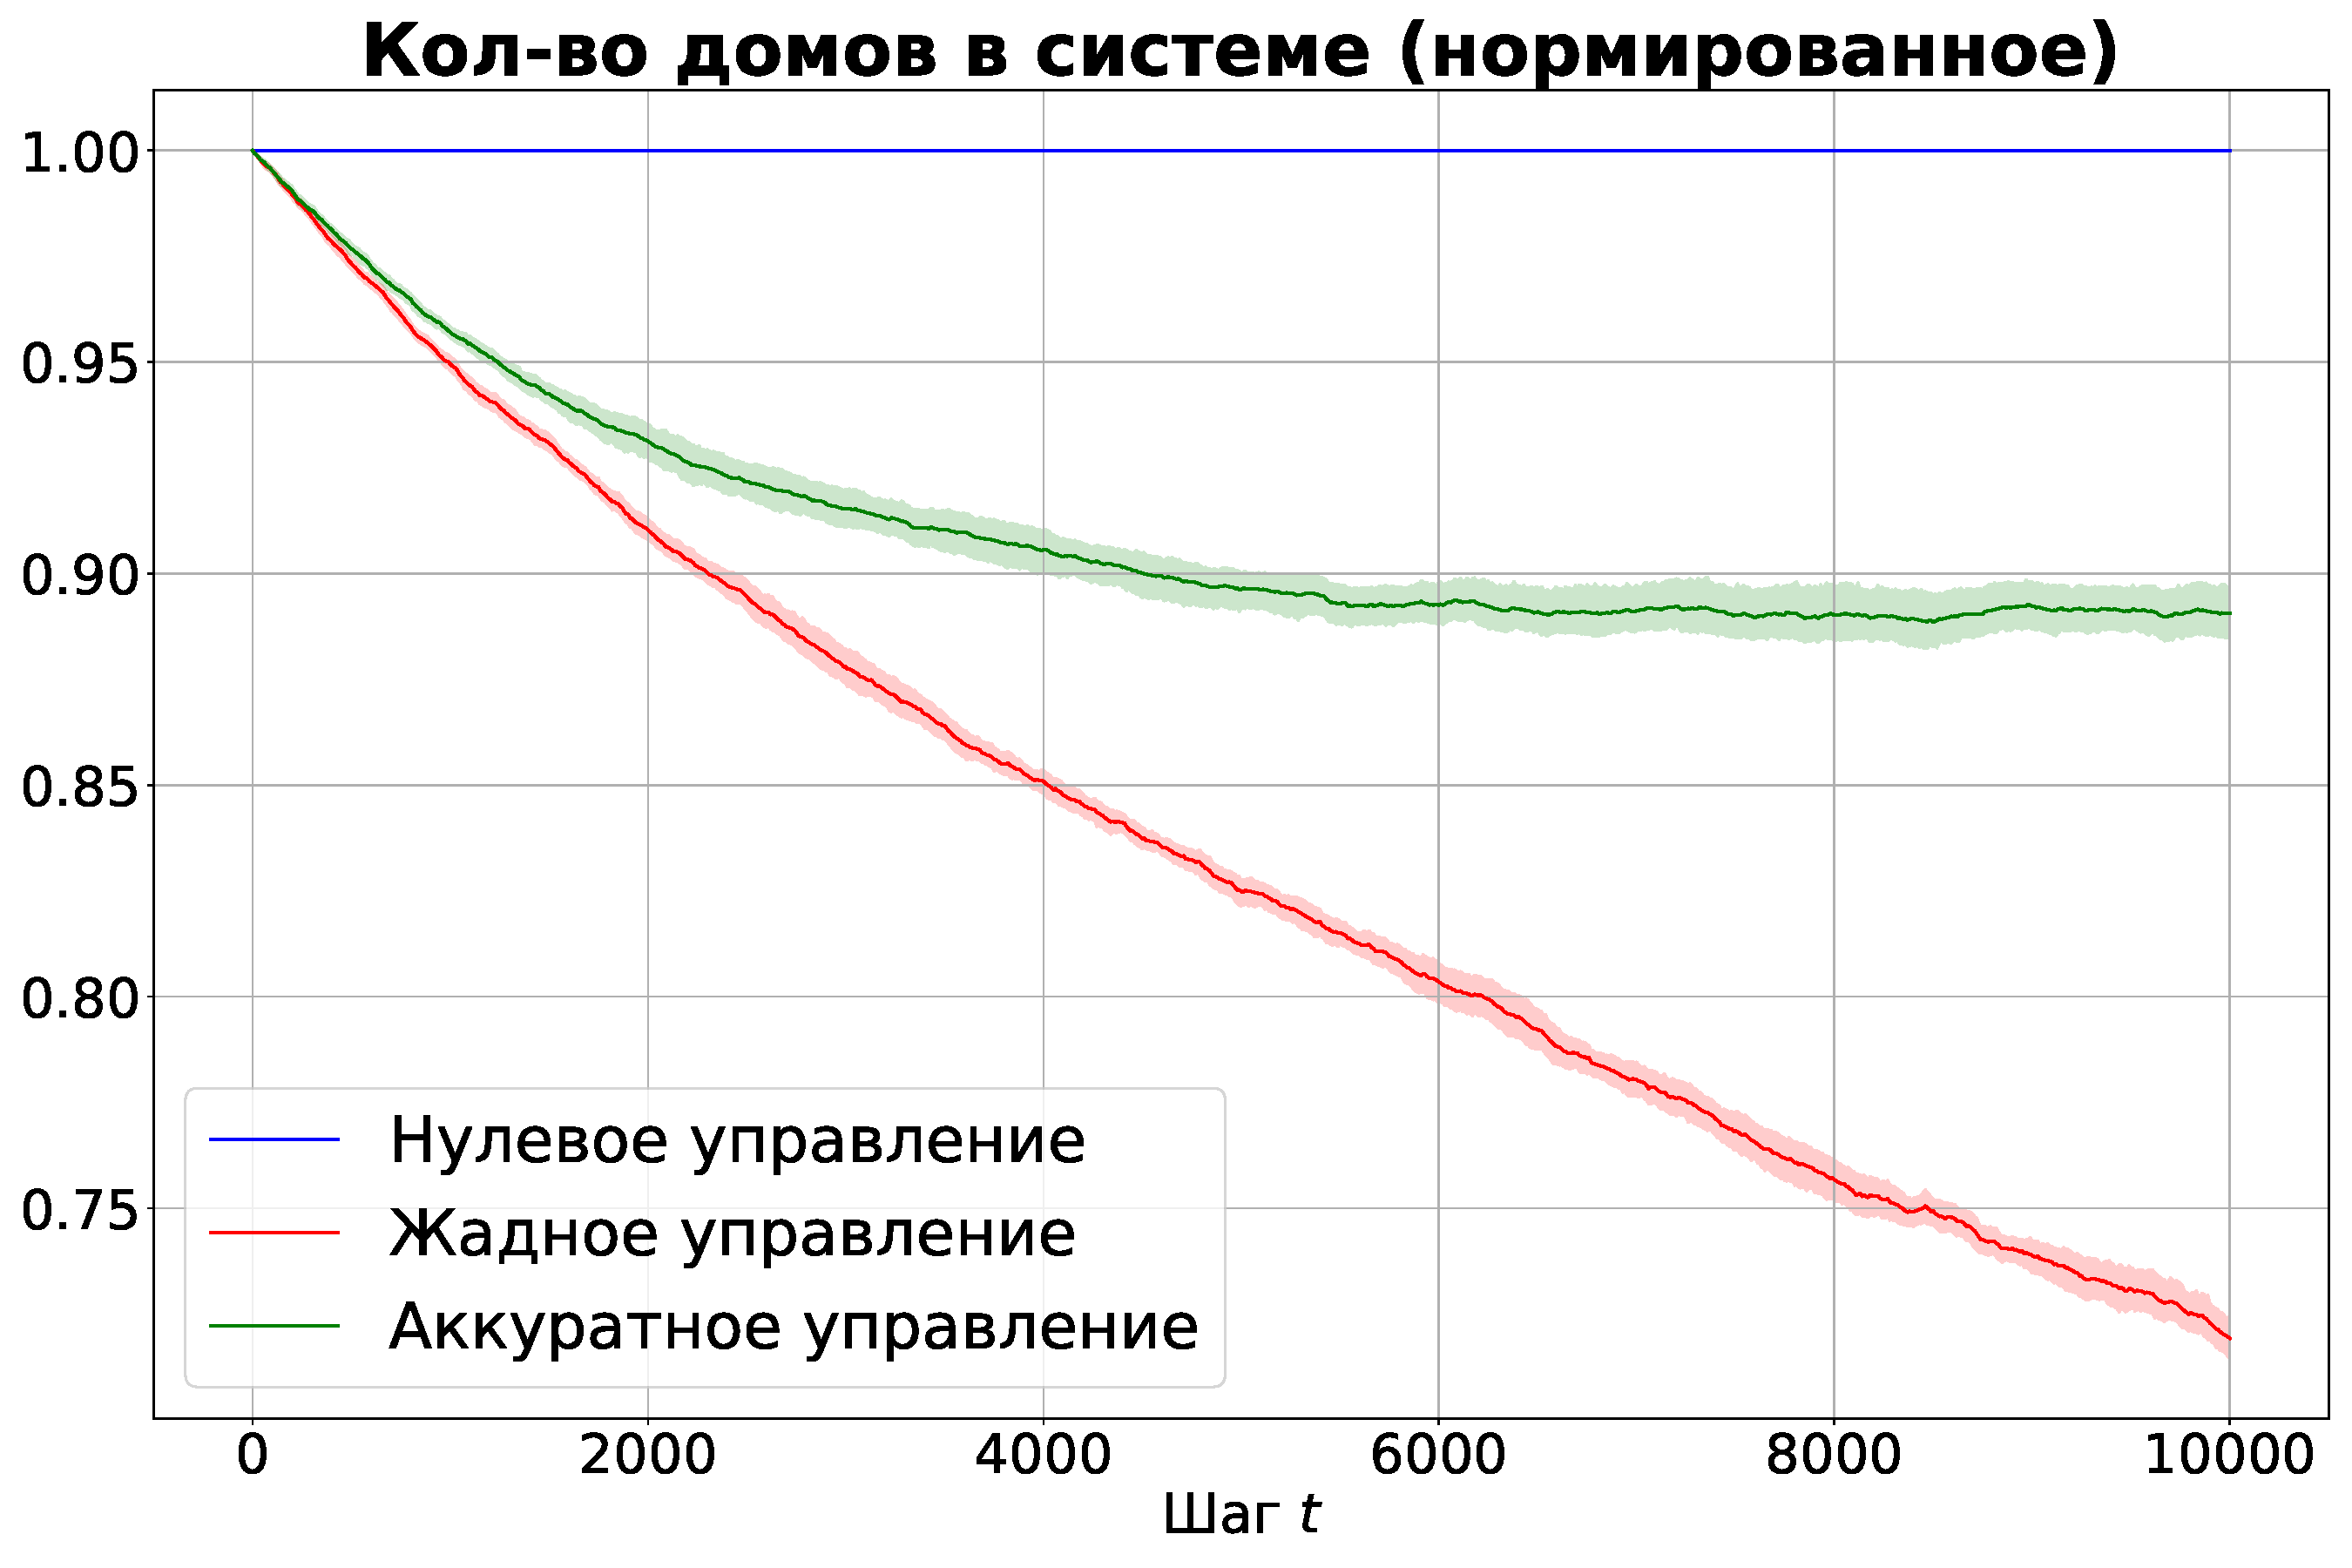
\includegraphics[width=0.48\linewidth]{N_california_smart_greedy_30.pdf}
    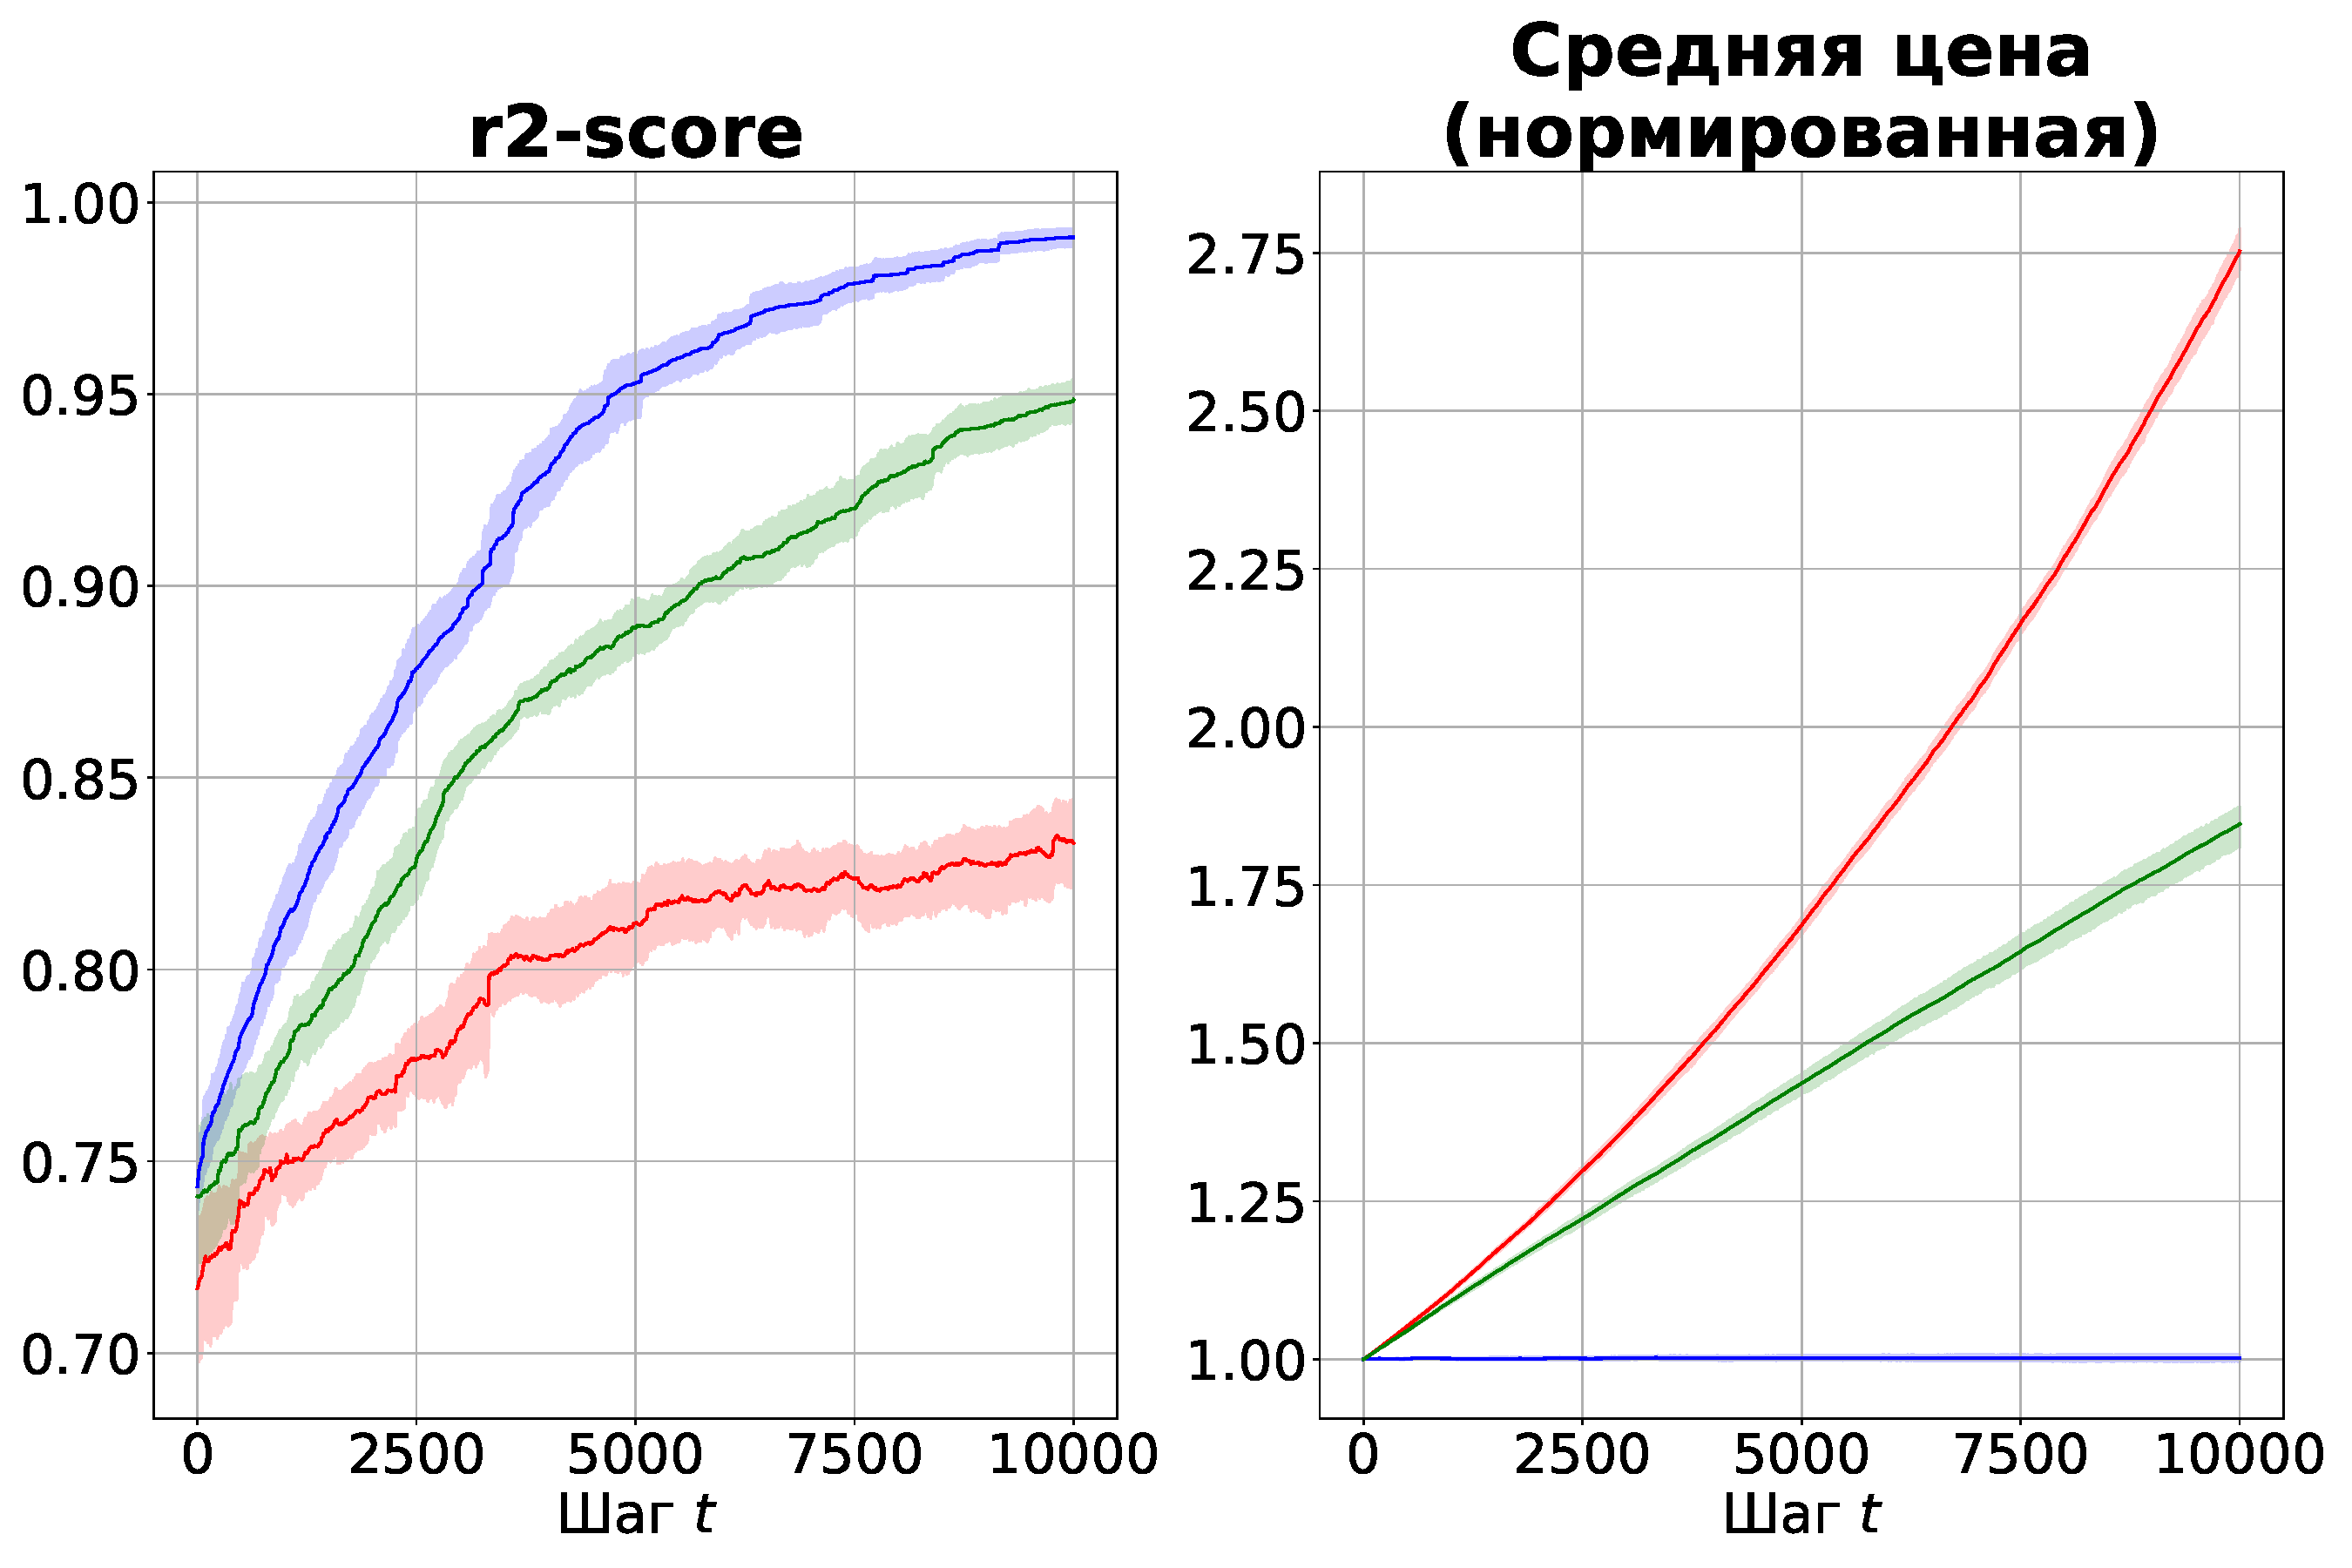
\includegraphics[width=0.48\linewidth]{r2-y_california_smart_greedy_30_N.pdf}
    \caption{Сравнение нулевого, наивной и аккуратной жадных стратегий на задаче прогнозирования цен. Слева приведен размер активной выборки $N_t$ как функция шага. Справа приведена метрика $R^2$ модели по целевой переменной на той же выборке. Синие кривые отвечают нулевому управлению $u_t \equiv 0$, при котором $N_t$ сохраняется и $R^2$ медленно растет за счет петли обратной связи. Красные кривые отвечают наивной жадной стратегии, которая ведет систему к деградации. Зеленые кривые отвечают аккуратной стратегии, которая сохраняет систему работоспособной.}
    \label{fig:degradation_results}
\end{figure}

Эксперимент подтверждает основной вывод подраздела~\ref{sec:degradation}. Условие $g$ в постановке \eqref{eq:g_cond}--\eqref{eq:opt} должно учитывать наблюдаемую выборку, а не только текущее состояние модели и среды. Без такой зависимости жадная стратегия максимизирует локальную метрику и одновременно разрушает систему. С зависимостью от наблюдаемой выборки та же стратегия сохраняет рост метрики и не теряет пользователей.

\subsection{Generative Replay в задаче непрерывного обучения}\label{sec:exp_gr}

В этом подразделе проверяются теоретические результаты подраздела~\ref{sec:gr} о методе Generative Replay. Сначала описывается единый протокол обучения для всех экспериментов и расписания управления, затем приводятся пять экспериментов: на квадратичной регрессии вне класса гипотез (подраздел~\ref{sec:exp_parabola}), на задаче с попарно ортогональными носителями гессианов (подраздел~\ref{sec:exp_svd}), на жадном выборе порядка задач (подраздел~\ref{sec:exp_greedy}), на линейной рекурсии с независимыми случайными оптимумами (подраздел~\ref{sec:exp_bv}) и на реальной задаче классификации медицинских изображений (подраздел~\ref{sec:exp_cxr}).

\subsubsection{Общий протокол обучения}\label{sec:exp_gr_setup}

Есть $T$ задач $D_1, \ldots, D_T$ с непересекающимися источниками данных. Через $\btheta^t$ обозначаются веса модели $m_{\btheta^t}$, увидевшей задачи $D_1, \ldots, D_t$, через $G_t$ обозначается генератор повторения, обученный по тем же $t$ задачам. Процесс задается последовательностью переходов
\[
    (\btheta^t, G_t) \longrightarrow (\btheta^{t+1}, G_{t+1}), \qquad t = 0, 1, \ldots, T-1.
\]
Один переход $\btheta^t \to \btheta^{t+1}$ определяется управлением $u_{t+1} \in [0, 1]$ и устроен в три шага. Формируется обучающий буфер $\cD_{t+1}$ длины $W$, в котором доля $u_{t+1}$ есть пары $(\bx, y) \sim D_{t+1}$ из новой задачи, а доля $1 - u_{t+1}$ есть пары $(\bx, m_{\btheta^t}(\bx))$ с $\bx \sim G_t$. На этом буфере запускается процедура минимизации функционала из начальной точки $\btheta^t$, дающая новые веса $\btheta^{t+1}$. Генератор $G_{t+1}$ обновляется так, чтобы в его носитель попадала задача $D_{t+1}$. На первом переходе генератор $G_0$ еще не определен, поэтому $u_1 = 1$ и буфер $\cD_1$ целиком состоит из $D_1$.

Схема одного перехода приведена на Рис.~\ref{fig:gr_scheme}.

\begin{figure}[h!]
\centering
\resizebox{\linewidth}{!}{%
\begin{tikzpicture}[
    >=Stealth, thick, font=\small,
    box/.style={draw, rounded corners=8pt, align=center, inner sep=8pt, minimum width=4.2cm, minimum height=1.4cm},
    diam/.style={draw, diamond, aspect=2.2, align=center, inner sep=2pt, minimum width=4.2cm, minimum height=1.6cm},
    lbl/.style={font=\footnotesize, align=center}
]
    \node[diam] (U) at (0, 4.6) {Новая задача $D_{t+1}$};
    \node[diam] (C) at (9.5, 4.6) {Управление $u_{t+1}$};
    \node[box]  (B) at (0, 0)   {Обучающий буфер $\cD_{t+1}$\\длины $W$};
    \node[box]  (M) at (9.5, 0) {Модель $m_{\btheta^{t+1}}$};

    \draw[->] (B.east) -- (M.west);
    \draw[->] (M.north) -- (C.south);
    \draw[->] (C.west) -- (U.east);
    \draw[->] (U.south) -- (B.north);

    \node[lbl, anchor=south] at ($(B.east)!0.5!(M.west) + (0, 0.1)$)
        {$N$ шагов минимизации\\$\btheta^t \to \btheta^{t+1}$};

    \node[lbl, anchor=west] at ($(M.north)!0.5!(C.south) + (0.2, 0)$)
        {обновление генератора\\$G_t \to G_{t+1}$};

    \node[lbl, above=1pt] at ($(C.west)!0.5!(U.east)$) {выбор источника};
    \node[lbl, below=1pt] at ($(C.west)!0.5!(U.east)$) {$u_{t+1}$ vs $1 - u_{t+1}$};

    \node[lbl, anchor=east, align=right] at ($(U.south)!0.5!(B.north) + (-0.2, 0)$)
        {доля $u_{t+1}$: $(\bx, y) \sim D_{t+1}$\\доля $1 - u_{t+1}$: $(\bx, m_{\btheta^t}(\bx))$,\\ $\bx \sim G_t$};

    \node[lbl, below=2pt] at ($(B.east)!0.5!(M.west)$) {$t \leftarrow t + 1$};
\end{tikzpicture}%
}
\caption{Один блок процесса Generative Replay. Управление $u_{t+1}$ задает долю новых данных в буфере $\cD_{t+1}$: с вероятностью $u_{t+1}$ берется пара из задачи $D_{t+1}$, с вероятностью $1 - u_{t+1}$ берется пара из генератора $G_t$ с меткой от текущей модели. На буфере выполняется $N$ шагов минимизации, дающих веса $\btheta^{t+1}$. Затем генератор обновляется до $G_{t+1}$.}
\label{fig:gr_scheme}
\end{figure}

\paragraph{Расписания управления.}
В экспериментах сравниваются три семейства расписаний $u_t$. Первое семейство $\texttt{inv}$ с параметром $\alpha > 0$ задает $u_t = \alpha/(t+1)$ при $t \ge 1$. По Утверждению~\ref{prop:inverse_gr} при $\alpha = 1$ оно дает равномерные веса задач $\alpha_s = 1/T$ в финальной модели, при $\alpha > 1$ поздние задачи получают чуть больший вес, при $\alpha < 1$ меньший. Второе семейство $\texttt{const}$ с параметром $u \in (0, 1)$ задает $u_t = u$ для всех $t \ge 1$. По Лемме~\ref{lem:weights_gr} веса образуют геометрическую последовательность $\alpha_s = u(1-u)^{T-s}$ при $s \ge 2$ и $\alpha_1 = (1-u)^{T-1}$. Третье семейство $\texttt{exp}$ с параметром $\alpha > 0$ задает $u_t = (e^{-\alpha t/(T-1)} - e^{-\alpha})/(1 - e^{-\alpha})$ при $t \ge 1$ и плавно убывает от $u_1 \approx 1$ до $u_{T-1} = 0$.

Графики трех семейств для нескольких значений параметра приведены на Рис.~\ref{fig:control_schedules}.

\begin{figure}[h!]
    \centering
    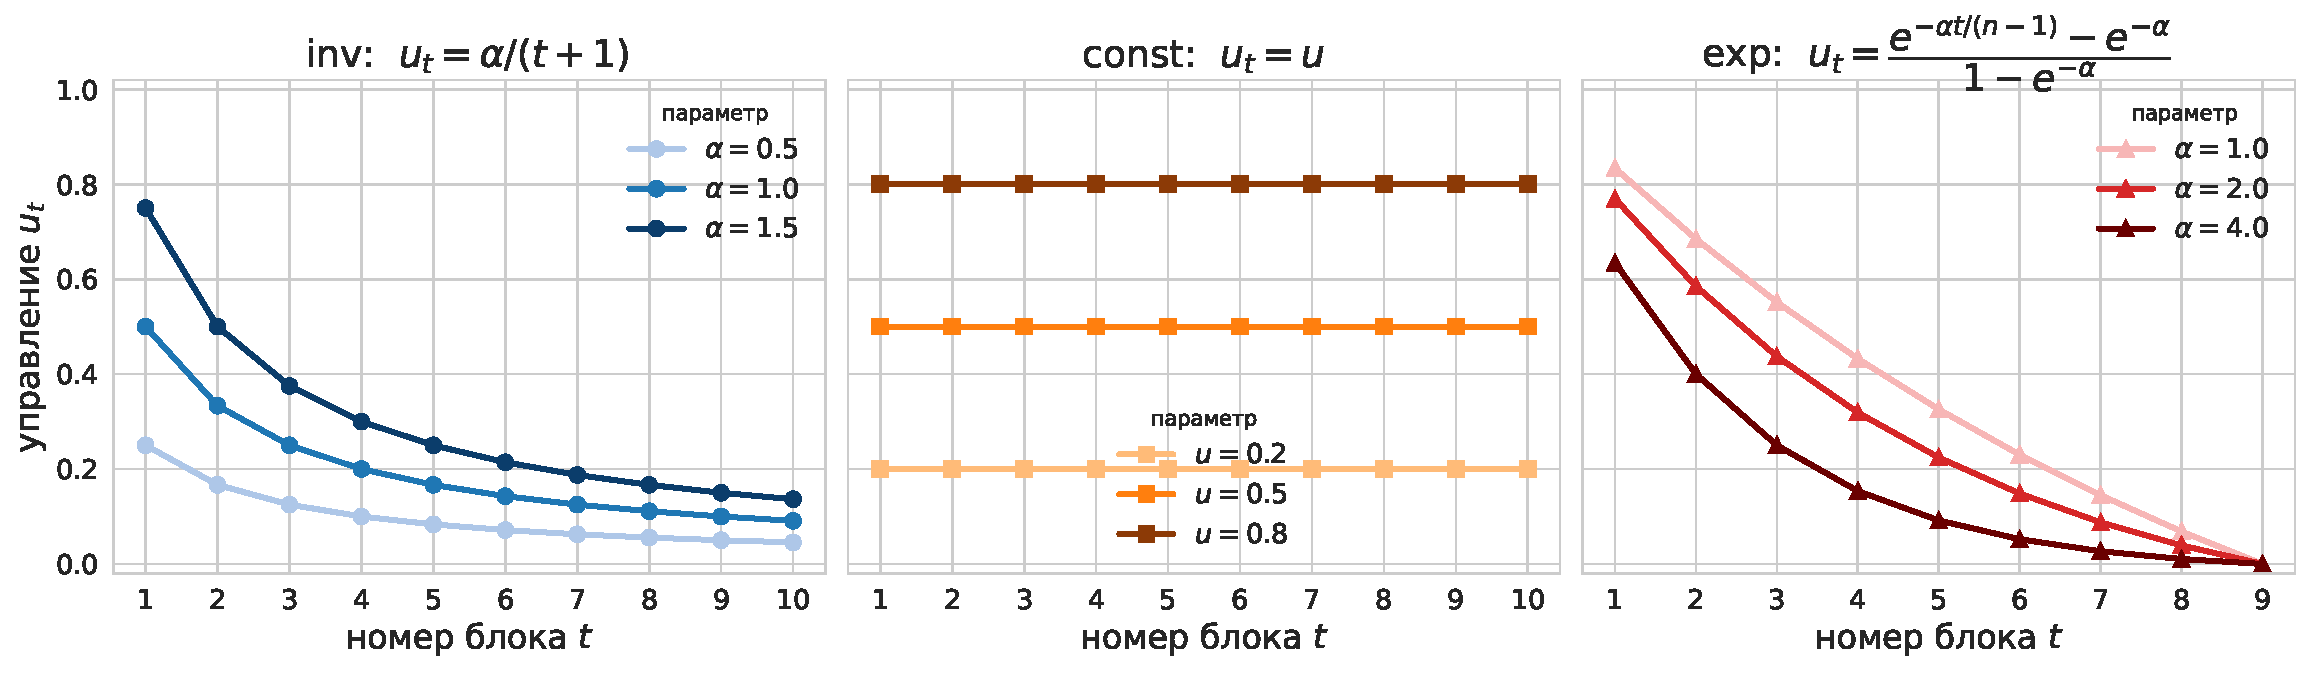
\includegraphics[width=\linewidth]{control_schedules.pdf}
    \caption{Три семейства расписаний $u_t$ как функции номера блока $t$ при $T = 10$. Слева расписание $\texttt{inv}$ с $\alpha \in \{0{,}5;\,1;\,1{,}5\}$, посередине $\texttt{const}$ с $u \in \{0{,}2;\,0{,}5;\,0{,}8\}$, справа $\texttt{exp}$ с $\alpha \in \{1;\,2;\,4\}$. Расписание $\texttt{inv}$ быстро убывает, $\texttt{const}$ остается постоянным, $\texttt{exp}$ плавно убывает до $u_{T-1} = 0$.}
    \label{fig:control_schedules}
\end{figure}

\subsubsection{Регрессия параболы линейной моделью}\label{sec:exp_parabola}

\paragraph{Что проверяется.}
Эксперимент проверяет монотонность средней ошибки из Теоремы~\ref{thm:avg_error_gr} и предсказание Утверждения~\ref{prop:inverse_gr} о соответствии расписаний весам задач. Расписание $\texttt{inv}$ с $\alpha = 1$ дает равномерные веса задач, $\texttt{const}$ дает геометрически убывающие веса с упором на поздние задачи. Ожидается, что при $\texttt{inv}$ ошибка по всем задачам выходит на уровень совместного обучения, при $\texttt{const}$ остается выше за счет просадки ранних задач.

\paragraph{Конструкция задач.}
Парабола $y = x^2$ разбита на $T = 10$ непересекающихся участков по $x$. Задача $D_s$ состоит из пар $(x_i, y_i)$ с $x_i \sim \mathrm{Uniform}[s, s+1]$ и $y_i = x_i^2$. В качестве модели используется линейная регрессия $\hat y = w_0 + w_1 x$, не способная точно воспроизвести квадратичную зависимость. Буфер $\cD_{t+1}$ длины $W = 500$, доля новых данных $u_{t+1} = 0{,}5$. Стохастический градиентный спуск с шагом $\eta = 10^{-2}$, $N = 500$ итераций на блок, усреднение по пяти реализациям.

\paragraph{Метрики.}
Записываются три величины: ошибка $\cL^{\mathrm{curr}}_t = \cL_t(\btheta^t)$ на текущей задаче, средняя ошибка $\cL_t = \tfrac{1}{t}\sum_{s=1}^t \cL_s(\btheta^t)$ по всем изученным задачам и совместный ориентир $\cL^{\mathrm{joint}}_T = \min_{\btheta}\tfrac{1}{T}\sum_{s=1}^T \cL_s(\btheta)$ для модели, обученной офлайн на $D_1 \cup \ldots \cup D_T$.

\paragraph{Результаты.}
На Рис.~\ref{fig:exp_parabola} приведены кривые $\cL^{\mathrm{curr}}_t$ и $\cL_t$ для трех расписаний. Величина $\cL_t$ монотонно снижается с поступлением новых блоков и асимптотически подходит к $\cL^{\mathrm{joint}}_T$. Расписания $\texttt{inv}$ и $\texttt{exp}$ дают одинаковый асимптотический уровень. Расписание $\texttt{const}$ сходится медленнее: постоянная доля повторения не учитывает накопленный объем прошлых задач.

\begin{figure}[h!]
    \centering
    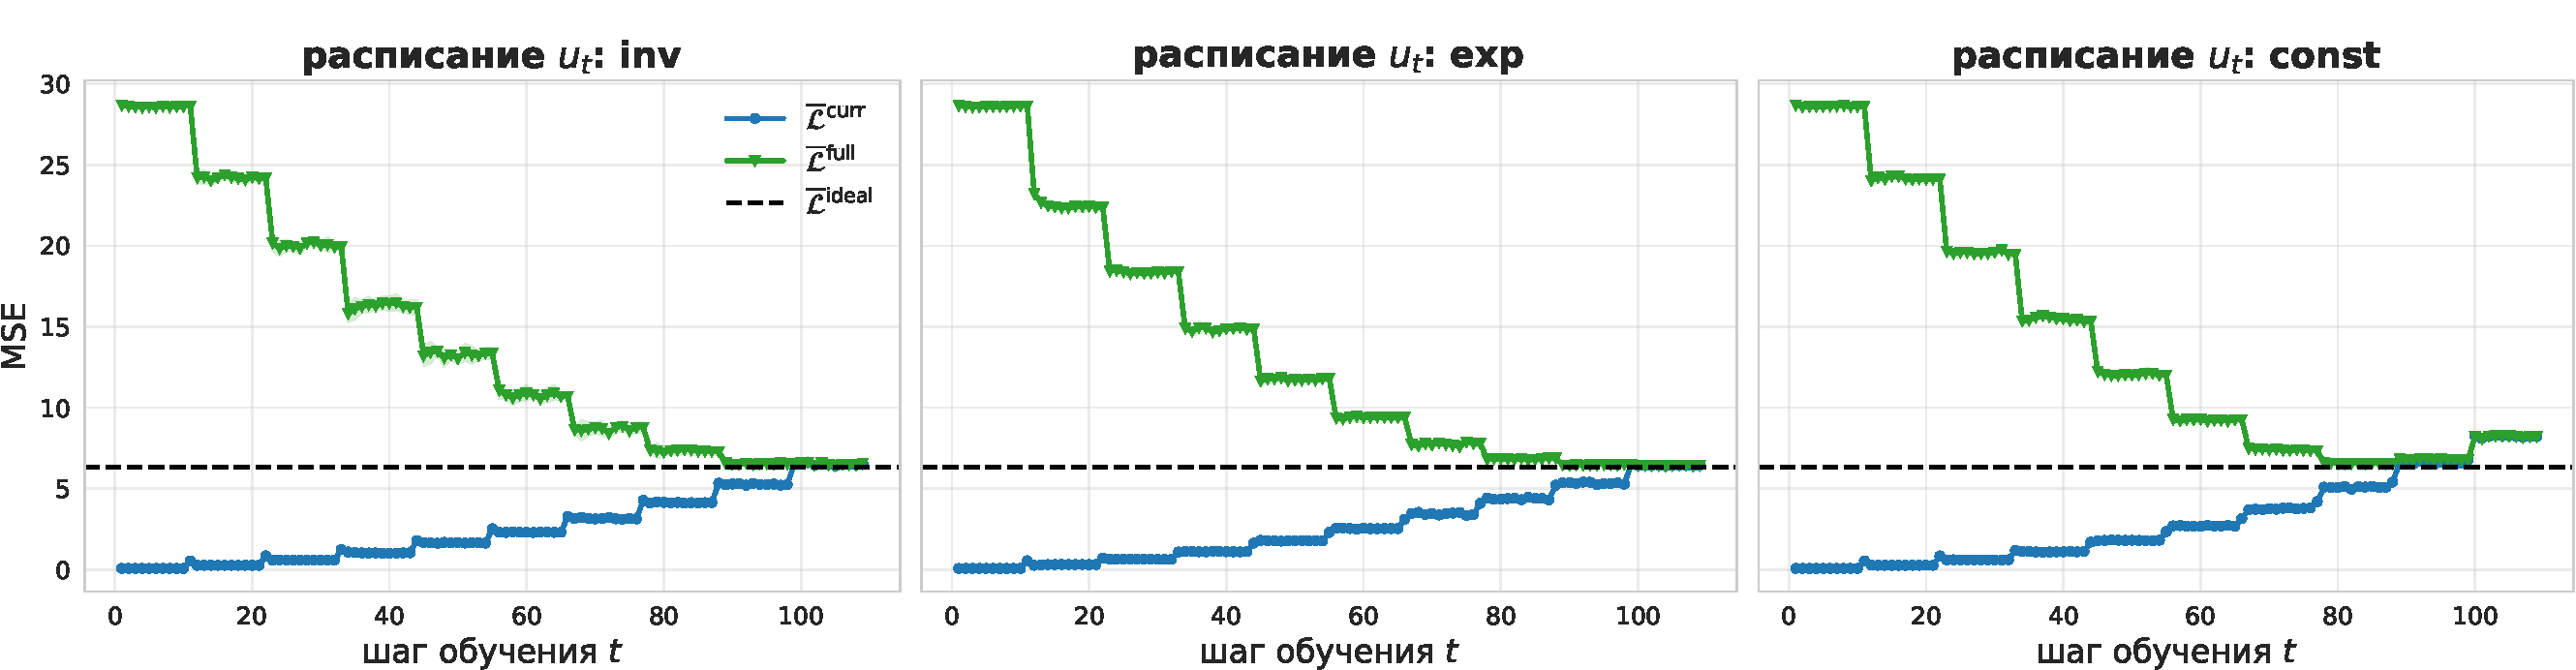
\includegraphics[width=\linewidth]{parabola_losses.pdf}
    \caption{Регрессия параболы линейной моделью: $\cL^{\mathrm{curr}}_t$ (синяя) и $\cL_t$ (зеленая) как функции шага обучения $t$ для трех расписаний $u_t$. Черный пунктир обозначает уровень совместного обучения $\cL^{\mathrm{joint}}_T$. Заливка показывает стандартное отклонение по пяти реализациям.}
    \label{fig:exp_parabola}
\end{figure}

\paragraph{Обсуждение.}
Картина согласуется с Теоремой~\ref{thm:avg_error_gr}: расписание с равномерными весами доставляет минимум верхней оценки средней ошибки. Геометрический вес ранних задач при $\texttt{const}$ экспоненциально мал по $T-s$, поэтому соответствующая кривая лежит выше $\texttt{inv}$ и не достигает уровня совместного обучения. Семейство $\texttt{exp}$ выходит на тот же уровень, что и $\texttt{inv}$ за счет близких к равномерным весов при выбранных параметрах. Эксперимент проверяет одновременно два теоретических предсказания: соответствие управления и весов задач из Утверждения~\ref{prop:inverse_gr} и оценку~\eqref{eq:LD2_gr} монотонности по $T$. Разрыв $\cL_T - \cL^{\mathrm{joint}}_T$ объясняется ограниченностью линейной модели на квадратичной целевой функции и составляет $\bar\varepsilon^*$ из спектральной теории.

\subsubsection{Ортогональные носители гессианов}\label{sec:exp_svd}

\paragraph{Что проверяется.}
Эксперимент проверяет Следствие~\ref{cor:zero_conflict_gr}: при попарной ортогональности носителей гессианов $\pi_t = 0$ и финальная ошибка не зависит от расписания. Конструкция SVD-задач делает условие $H_{t+1}\Sigma_t = 0$ явным: оптимум каждой задачи лежит на одной координате общего ортогонального базиса.

\paragraph{Конструкция задач.}
Случайная ортонормированная матрица $V \in \bbR^{T \times T}$ имеет столбцы $v_1, \ldots, v_T$. Задача $D_s$ задается выборкой $X_s = \sigma_s\, z_s\, v_s^\top$, $Y_s = \sigma_s\, z_s$, где $z_s \in \bbR^N$ есть случайный единичный вектор. Совместный оптимум $w^{\mathrm{joint}} = \sum_s v_s$ доставляет нулевую ошибку на всех задачах. Параметры: $T = 10$, $W = 300$, $u_{t+1} = 0{,}5$, $\eta = 10^{-2}$, $N = 300$ итераций на блок, пять реализаций.

\paragraph{Результаты.}
На Рис.~\ref{fig:exp_svd} приведены кривые $\cL^{\mathrm{curr}}_t$ и $\cL_t$ для трех расписаний. Появление новой задачи порождает короткий всплеск $\cL^{\mathrm{curr}}_t$, который спадает после нескольких шагов градиентного спуска. Кривая $\cL_t$ монотонно убывает к нулю, поскольку ортогональность направлений $v_s$ дает $\cL^{\mathrm{joint}}_T = 0$.

\begin{figure}[h!]
    \centering
    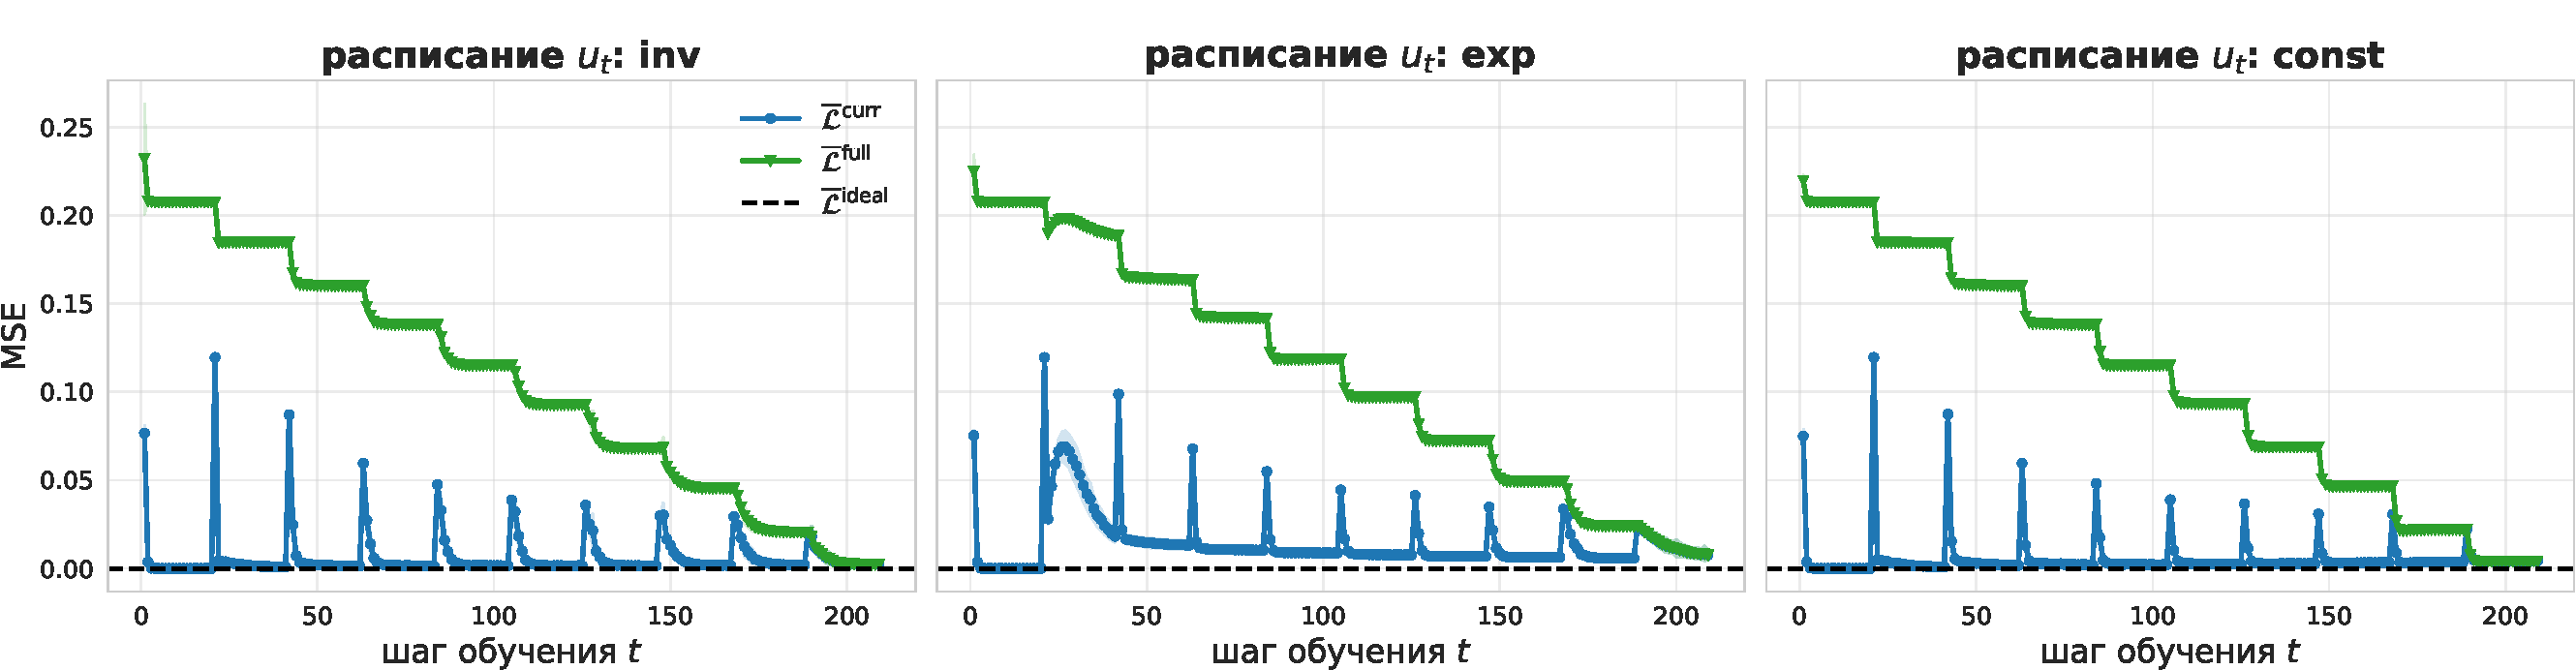
\includegraphics[width=\linewidth]{svd_losses.pdf}
    \caption{Ортогональные носители гессианов: $\cL^{\mathrm{curr}}_t$ (синяя) и $\cL_t$ (зеленая) как функции шага обучения $t$ для трех расписаний $u_t$. Черный пунктир обозначает $\cL^{\mathrm{joint}}_T = 0$. Заливка показывает стандартное отклонение по пяти реализациям.}
    \label{fig:exp_svd}
\end{figure}

\paragraph{Обсуждение.}
Все три расписания решают задачу примерно одинаково и выходят на $\cL_T \to 0$, при этом $\texttt{inv}$ устойчиво держится чуть ниже остальных по $\cL^{\mathrm{curr}}_t$ за счет более плавного изменения весов поздних задач. Сопоставимость траекторий подтверждает Следствие~\ref{cor:zero_conflict_gr}: при ортогональных носителях гессианов величина $\pi_t$ равна нулю, и финальная ошибка не зависит от выбора расписания. Это контрольный эксперимент. Если бы кривые расписаний начали расходиться в этой постановке, это указывало бы на нарушение условия ортогональности или на численные эффекты конечного числа шагов градиентного спуска. Ни того, ни другого в пределах пяти реализаций не наблюдается.

\subsubsection{Жадный выбор порядка задач}\label{sec:exp_greedy}

\paragraph{Что проверяется.}
Эксперимент проверяет следующее предсказание спектральной теории. По безусловной оценке из Теоремы~\ref{thm:unconditional_gr} верхняя оценка финальной ошибки зависит от перестановки задач $\sigma$ только через сумму $\sum_t \|\Delta_t\|^2$, где $\Delta_t = \btheta^*_{\sigma(t+1)} - \btheta^t$. Жадная стратегия выбора порядка локально минимизирует эту сумму и должна доставлять меньшее $\cL_T$ среди стратегий без знания будущих шагов. По Лемме~\ref{lem:gr_step} при точной внутренней минимизации финальное состояние $\btheta^T$ не зависит от порядка, поэтому эффект порядка локализован в канале неточной внутренней минимизации.

\paragraph{Конструкция.}
Размерность параметра $d = 50$, число задач $T \in \{3, 4, 5, 6, 7\}$. Гессианы задаются разложением $H_s = U_s \Lambda_s U_s^\top$ со случайной ортогональной $U_s \in \mathrm{O}(d)$ и собственными значениями $\lambda_{s,i} \sim \mathrm{LogUnif}[1, 10]$. Оптимумы задач задаются так:
\[
    \btheta^*_s \sim 0{,}1 \cdot \cN(0, I_d) \text{ при } s \ne s^*, \qquad \btheta^*_{s^*} = \frac{R}{\sqrt d}\xi, \quad \xi \sim \cN(0, I_d), \quad R = 20,
\]
индекс выделенной задачи $s^*$ выбирается равновероятно. Потери квадратичны: $\cL_s(\btheta) = \tfrac{1}{2}\|\btheta - \btheta^*_s\|^2_{H_s}$. На каждом переходе делается один шаг градиентного спуска с шагом $\eta_t = 0{,}5/\lambda_{\max}(M_t)$, что моделирует режим неточной внутренней минимизации.

\paragraph{Сравниваемые стратегии.}
Жадная стратегия $\sigma_{\mathrm{gr}}(t+1) = \arg\min_s \|\btheta^*_s - \btheta^t\|$ среди оставшихся задач, случайный порядок (усреднение по $200$ выборкам), антижадная стратегия $\sigma_{\mathrm{anti}}(t+1) = \arg\max_s \|\btheta^*_s - \btheta^t\|$ как опорная и оптимальный порядок (полный перебор $T!$ перестановок). Для каждого значения $T$ усреднение проводится по $30$ независимым реализациям набора задач.

\paragraph{Результаты.}
На Рис.~\ref{fig:greedy_ordering} приведена зависимость средней финальной ошибки $\cL_T$ от числа задач для четырех стратегий и теоретического ориентира $\cL_T^{\mathrm{joint}}$ совместного обучения.

\begin{figure}[h!]
    \centering
    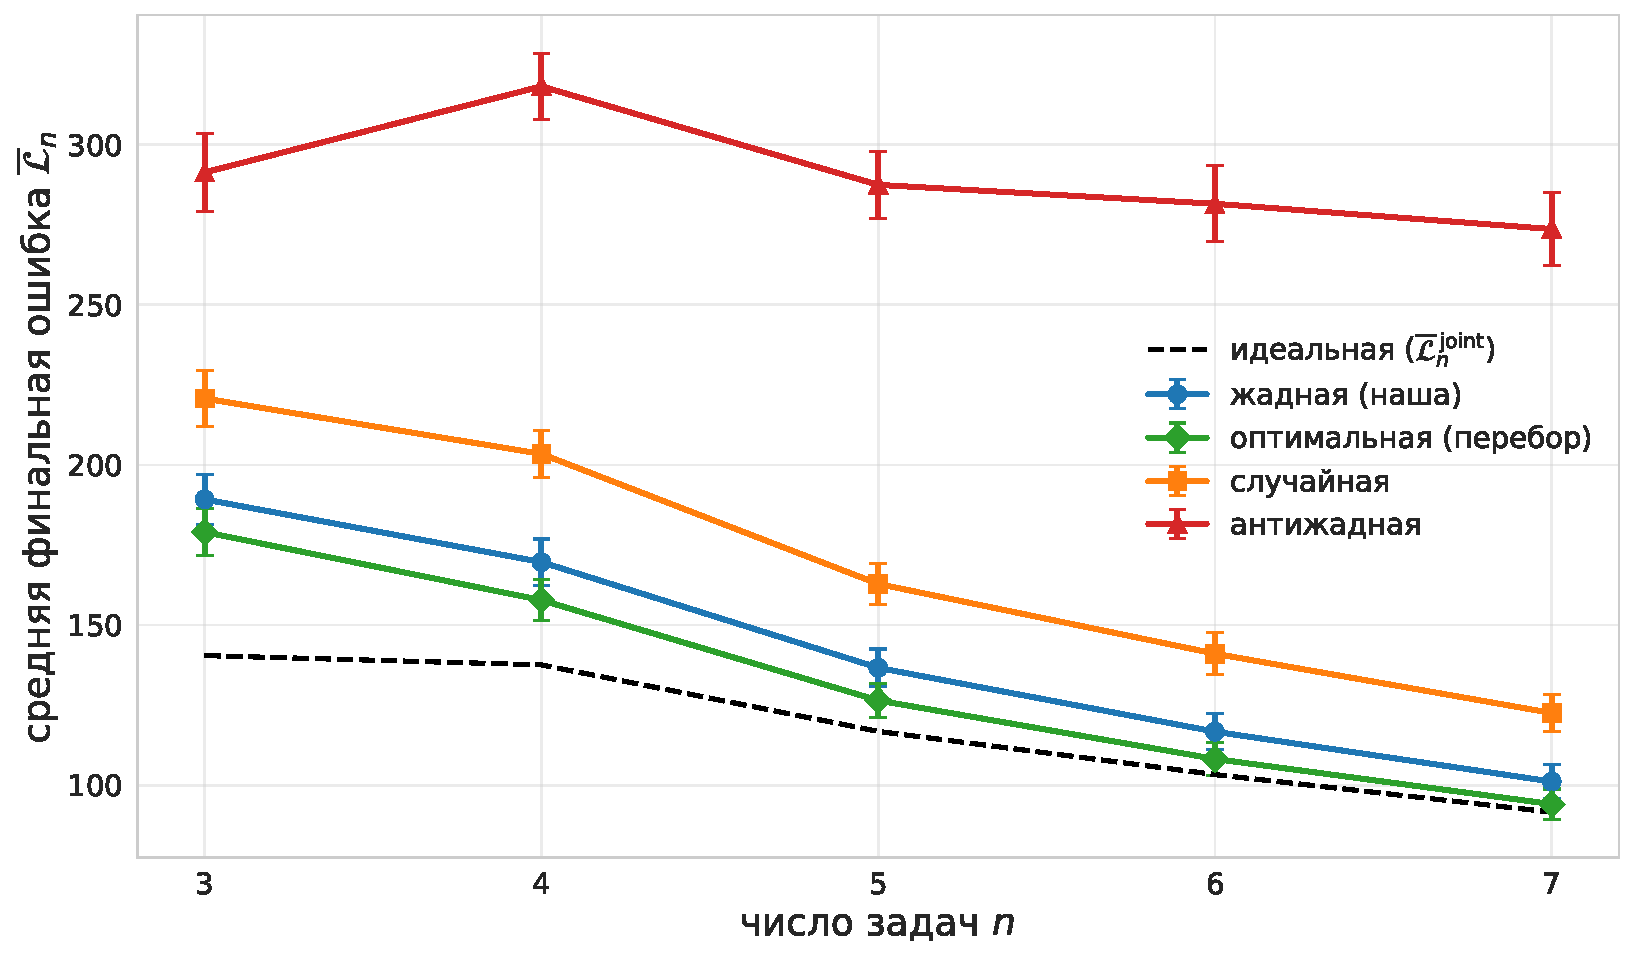
\includegraphics[width=0.85\linewidth]{T_sweep_greedy_ordering.pdf}
    \caption{Средняя финальная ошибка $\cL_T$ как функция числа задач $T$ для жадного, случайного, антижадного и оптимального порядков. Черный пунктир показывает теоретический ориентир совместного обучения $\cL_T^{\mathrm{joint}}$. Усы соответствуют стандартной ошибке среднего по $30$ независимым реализациям.}
    \label{fig:greedy_ordering}
\end{figure}

\paragraph{Обсуждение.}
Жадная стратегия располагается между оптимальной и случайной, ближе к оптимальной. Расхождение со случайным порядком составляет $14$--$18\%$ от $\cL_T^{\mathrm{random}}$, антижадная отстает на $54$--$171\%$. Разрыв с оптимальной стратегией составляет $6$--$8\%$, что заметно меньше отрыва от случайного порядка. Это подтверждает прогноз Теоремы~\ref{thm:unconditional_gr}: локальная минимизация $\|\Delta_t\|^2$ переносится на финальную ошибку. Эффект полностью локализован в канале неточной внутренней минимизации, что согласуется с Леммой~\ref{lem:gr_step}: если бы внутренняя минимизация была точной, финальное состояние не зависело бы от порядка вовсе. С ростом $T$ все стратегии сближаются с ориентиром $\cL_T^{\mathrm{joint}}$, поскольку увеличение числа задач уменьшает удельный вклад каждой из них в среднюю ошибку.

\subsubsection{Bias-variance разложение}\label{sec:exp_bv}

\paragraph{Что проверяется.}
Эксперимент проверяет точность разложения из Теоремы~\ref{thm:bv_gr} и разделение режимов из Теоремы~\ref{thm:convergence_gr}: $\sum_t u_t = \infty$ отвечает за обнуление смещения, а $u_t \to 0$ в сочетании с первым условием за обнуление дисперсии. Сравнивается эмпирическое значение $\bbE\|\btheta^t - \mu^*\|^2$ с теоретической формулой.

\paragraph{Конструкция.}
Квадратичный случай Предположений~\ref{ass:common_H_gr} и~\ref{ass:iid_targets_gr}: $H = I_d$ при $d = 20$, оптимумы $\btheta^*_s \sim \cN(0, I_d)$, $\mu^* = 0$, $\mathrm{tr}(C^*) = 20$, $\btheta^0 = (1, \ldots, 1)$. Внутренняя минимизация заменяется точным решением: $\btheta^{t+1} = (1 - u_t)\btheta^t + u_t\btheta^*_{t+1}$. Усреднение по $K = 3000$ реализациям, $T = 10^5$ блоков.

\paragraph{Расписания.}
Сравниваются пять расписаний, покрывающих три режима Теоремы~\ref{thm:convergence_gr}:
\begin{itemize}
    \item $\texttt{inv}$ с $u_t = 1/(t+2)$: одновременно $\sum_t u_t = \infty$ и $u_t \to 0$, ожидаемый режим bias $\to 0$, variance $\to 0$ со скоростью $\mathcal{O}(1/t)$.
    \item $\texttt{const}$ с $u \in \{0{,}2;\,0{,}5;\,0{,}8\}$: $\sum_t u_t = \infty$, но $u_t \not\to 0$. Ожидаемый режим bias $\to 0$ экспоненциально, variance $\to \tfrac{u}{2-u}\mathrm{tr}(C^*) \in \{2{,}22;\,6{,}67;\,13{,}33\}$.
    \item $\texttt{quad}$ с $u_t = 1/(t+2)^2$: расписание суммируемо, $\sum_t u_t < \infty$. Ожидаемый режим: bias и variance выходят на ненулевое плато.
\end{itemize}

\paragraph{Результаты.}
На Рис.~\ref{fig:exp_bias_variance} показаны три панели для пяти расписаний. На финальном шаге $t = T$ отношение эмпирического MSE к теоретическому остается в пределах $0{,}3\%$ для всех расписаний: $\texttt{inv}$ дает $0{,}992$, $\texttt{const}$ с $u \in \{0{,}2;\,0{,}5;\,0{,}8\}$ дает $1{,}003$, $1{,}000$, $0{,}999$, $\texttt{quad}$ дает $1{,}000$. Стационарная дисперсия для $\texttt{const}$ на сетке $u \in \{0{,}1;\,0{,}3;\,0{,}5;\,0{,}7;\,0{,}9\}$ совпадает с теоретической $\tfrac{u}{2-u}\mathrm{tr}(C^*)$ в пределах $0{,}1\%$.

\begin{figure}[h!]
    \centering
    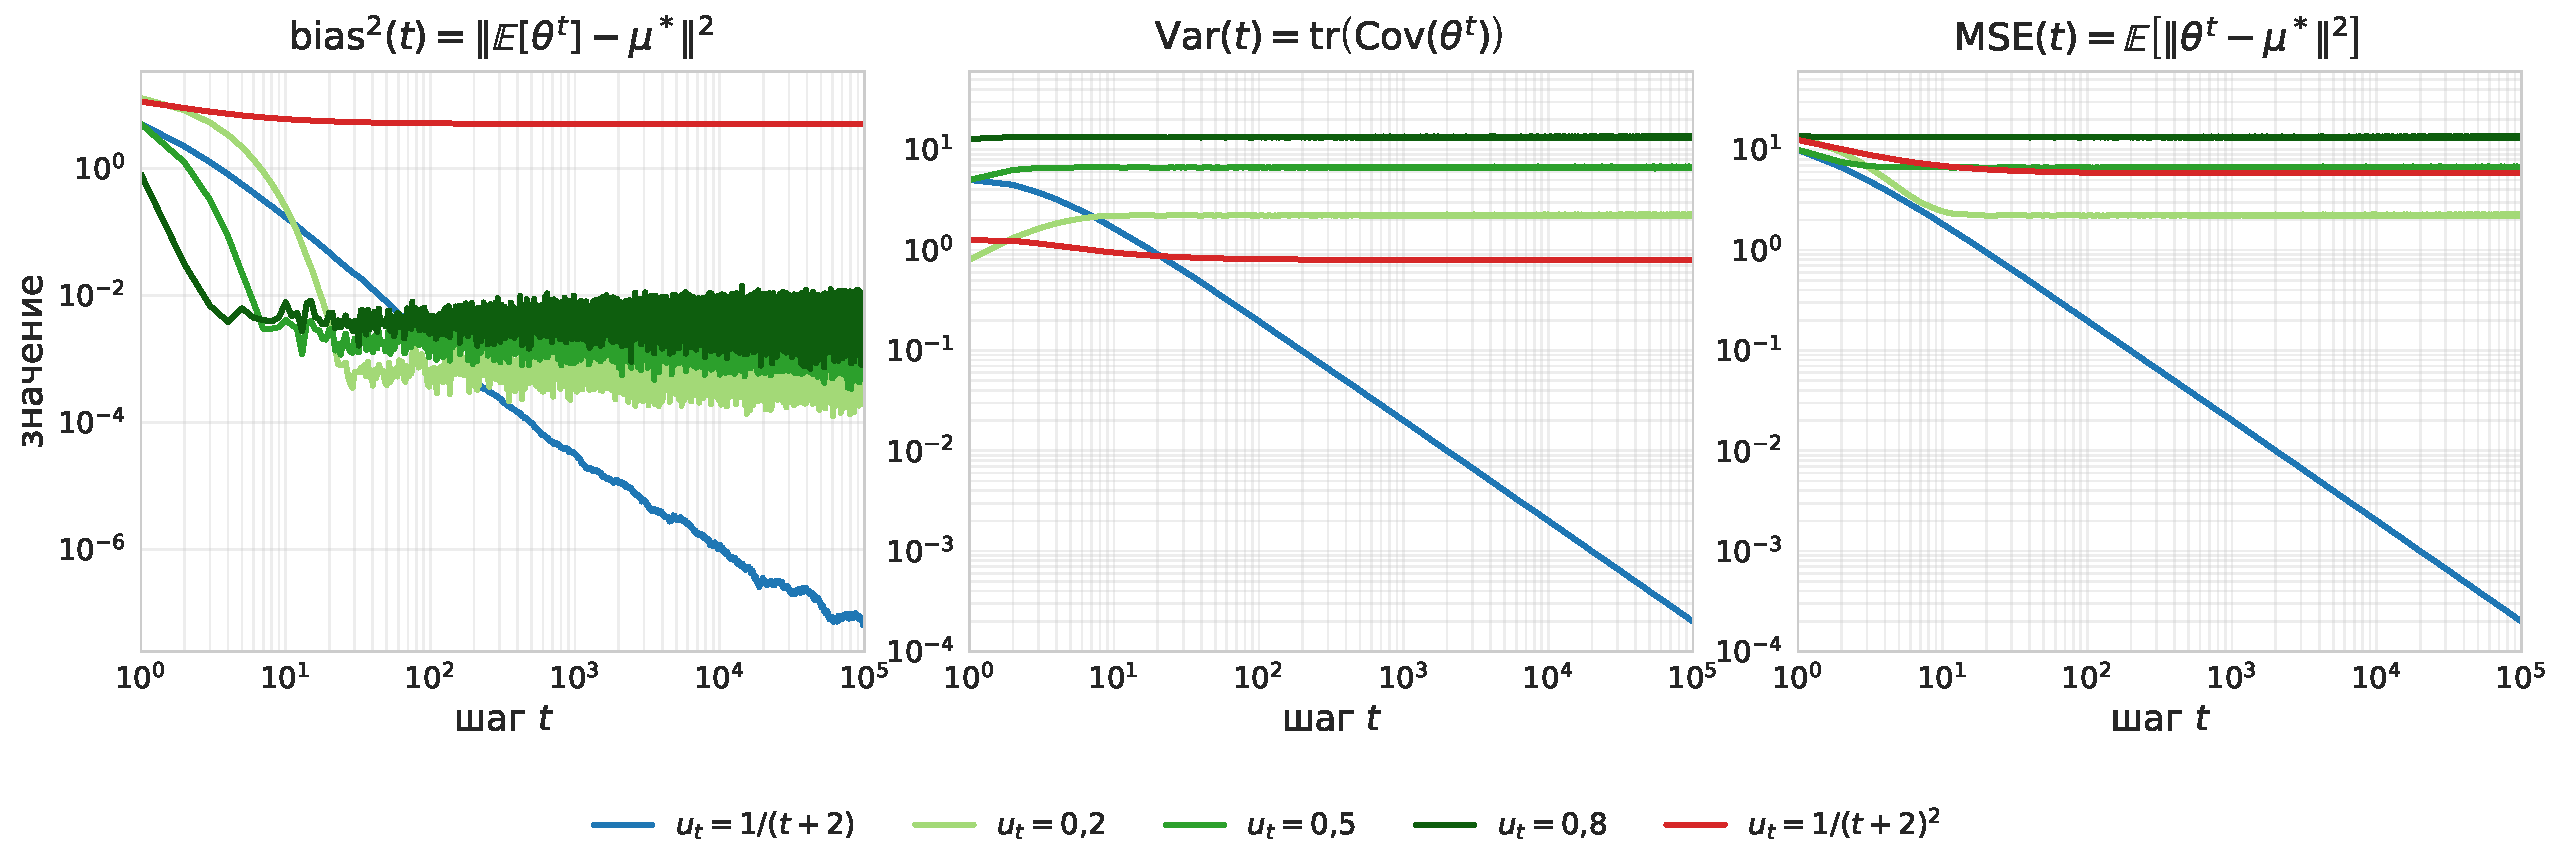
\includegraphics[width=\linewidth]{bias_variance.pdf}
    \caption{Bias-variance разложение в линейной рекурсии с независимыми оптимумами при $H = I_d$, $d = 20$, $T = 10^5$, $K = 3000$. Слева приведено $\mathrm{bias}^2(t) = \|\bbE[\btheta^t] - \mu^*\|^2$, посередине $\mathrm{Var}(t) = \mathrm{tr}\,\mathrm{Cov}(\btheta^t)$, справа $\mathrm{MSE}(t) = \bbE\|\btheta^t - \mu^*\|^2$. Расписание $\texttt{inv}$ обнуляет обе компоненты, семейство $\texttt{const}$ обнуляет смещение и удерживает дисперсию на стационарном уровне $\tfrac{u}{2-u}\mathrm{tr}(C^*)$, $\texttt{quad}$ оставляет обе компоненты на ненулевом плато.}
    \label{fig:exp_bias_variance}
\end{figure}

\paragraph{Обсуждение.}
Расписание $\texttt{inv}$ обнуляет обе компоненты со скоростью $\mathcal{O}(1/t)$ и устойчиво дает наименьшее MSE среди сравниваемых стратегий. Семейство $\texttt{const}$ обнуляет смещение экспоненциально, но удерживает дисперсию на стационарном уровне $\tfrac{u}{2-u}\mathrm{tr}(C^*)$, монотонно растущем с $u$: большой $u$ ускоряет забывание ранних задач ценой постоянного шума. Расписание $\texttt{quad}$ нарушает $\sum_t u_t = \infty$ и оставляет смещение на ненулевом плато. Совпадение эмпирических кривых с теоретической формулой в пределах $0{,}3\%$ при $K = 3000$ реализациях показывает, что разложение Теоремы~\ref{thm:bv_gr} обладает достаточной точностью, чтобы служить руководящим принципом при выборе расписания в задачах с независимыми оптимумами и общим гессианом. Эксперимент явно разделяет три режима из Теоремы~\ref{thm:convergence_gr} и подтверждает эквивалентность условиям Роббинса-Монро.

\subsubsection{ChestX-Ray}\label{sec:exp_cxr}

\paragraph{Датасет.}
Используется датасет NIH ChestX-Ray~\cite{wang2017chestx}: рентгеновские снимки грудной клетки с разметкой по $14$ диагнозам и классом <<норма>>. Отобраны пять патологий (Atelectasis, Cardiomegaly, Consolidation, Edema, Effusion) как пять задач $D_1, \ldots, D_5$ бинарной классификации соответствующего диагноза против остальных снимков. Класс <<норма>> играет роль начального состояния. Для каждой задачи берется $N = 4000$ обучающих снимков и независимая тестовая выборка.

\paragraph{Модель и обучение.}
В качестве модели используется MobileNetV2~\cite{sandler2018mobilenetv2} с головой, предобученной на ImageNet. Снимки размера $224 \times 224$, оптимизатор Adam~\cite{kingma2014adam} с шагом $\eta = 3 \cdot 10^{-4}$ и размером минибатча $64$, $25$ эпох на блок, буфер длины $W = 4000$. Повторение реализуется через сохраненный буфер представительных примеров уже изученных задач с псевдо-метками, восстанавливаемыми текущей моделью.

\paragraph{Метрика.}
В качестве метрики используется AUC по каждой из шести болезней. Сводные величины: Avg6 как средний AUC по всем шести болезням, Avg5 как средний AUC по пяти патологиям без класса <<норма>>. Верхний ориентир: совместное обучение $\texttt{multiclass}$ без разбиения на блоки.

\paragraph{Сравниваемые стратегии.}
К трем расписаниям $\texttt{inv}$, $\texttt{const}$, $\texttt{exp}$ добавляется адаптивная стратегия $\texttt{adaptive}$ из~\eqref{eq:adaptive_u}:
\[
    u_t = \mathrm{clip}\!\left(\frac{r_t}{r_t + \lambda g_t}, u_{\min}, u_{\max}\right),
\]
где $r_t$ есть потеря на текущей задаче, $g_t$ есть средняя потеря на изученных задачах, $u_{\min} = 0{,}05$, $u_{\max} = 0{,}95$. Усреднение по пяти запускам с разными начальными значениями случайного генератора.

\paragraph{Сводное сравнение.}
На Рис.~\ref{fig:cxr_summary_avg6} и Рис.~\ref{fig:cxr_summary_avg5} приведено сравнение стратегий по двум метрикам. Лучший результат дает расписание $\texttt{inv}$ с $\alpha = 1{,}5$: Avg6 $= 0{,}758 \pm 0{,}011$, Avg5 $= 0{,}782 \pm 0{,}010$. Разрыв с $\texttt{multiclass}$ ориентиром $5{,}5$ и $5{,}1$ процентных пункта. Следом идут $\texttt{adaptive}$ с $\lambda = 1$ и $\texttt{const}$ с $u = 0{,}62$.

\begin{figure}[h!]
    \centering
    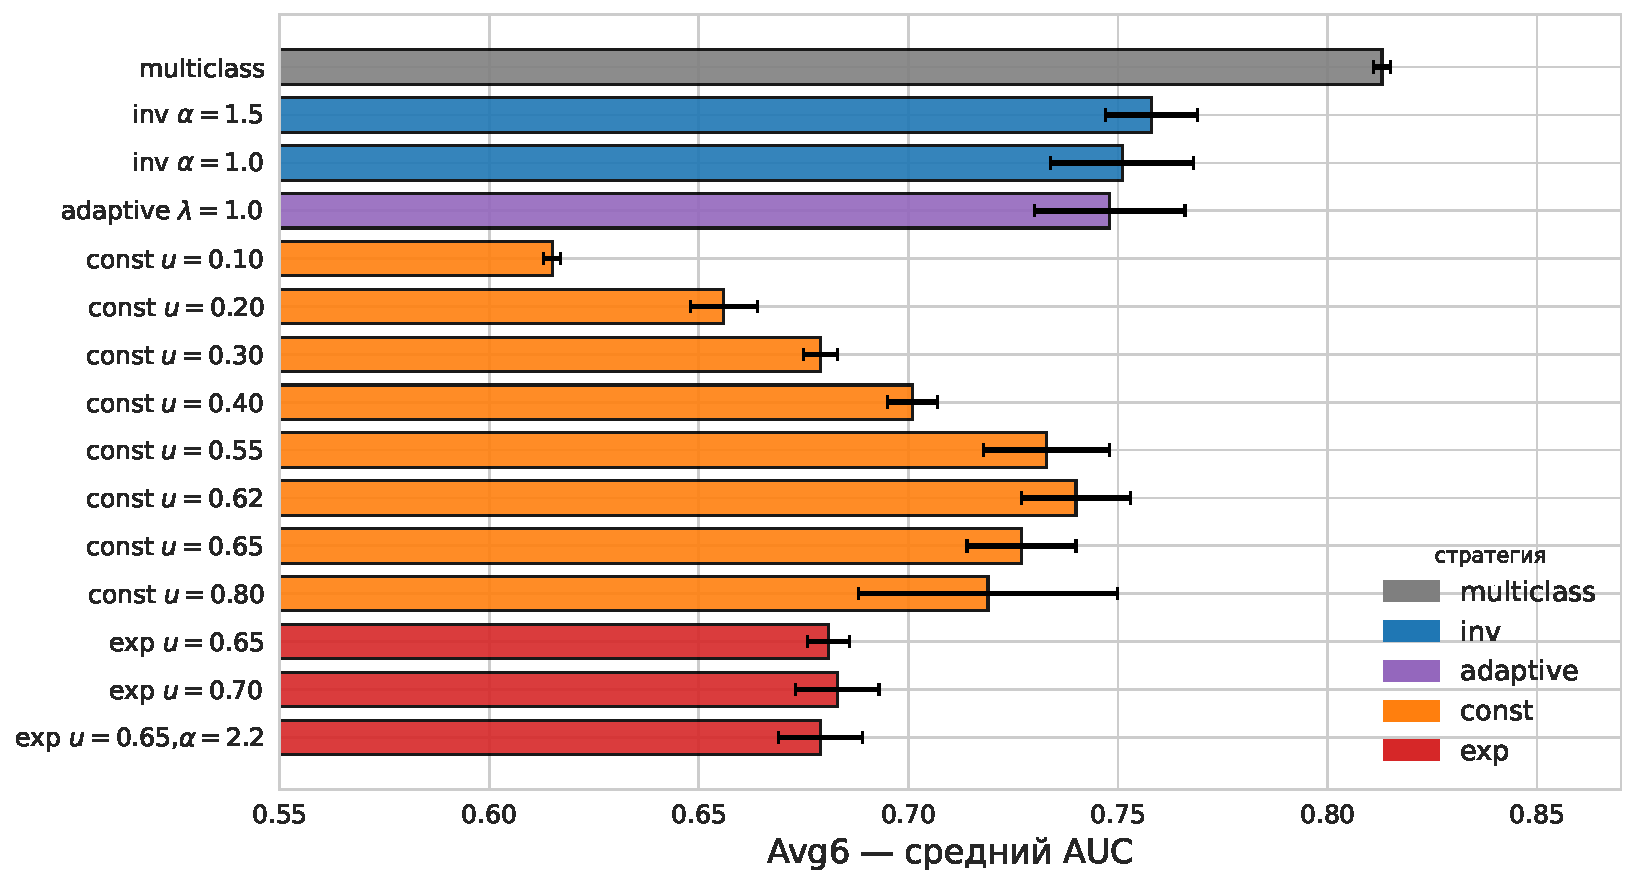
\includegraphics[width=0.92\linewidth]{cxr_summary_bar.pdf}
    \caption{Сводное сравнение стратегий $u_t$ по метрике Avg6 (средний AUC по шести болезням). Цвет полоски кодирует семейство стратегий, серая полоска $\texttt{multiclass}$ показывает верхний ориентир совместного обучения. Усы соответствуют стандартному отклонению по пяти независимым запускам.}
    \label{fig:cxr_summary_avg6}
\end{figure}

\begin{figure}[h!]
    \centering
    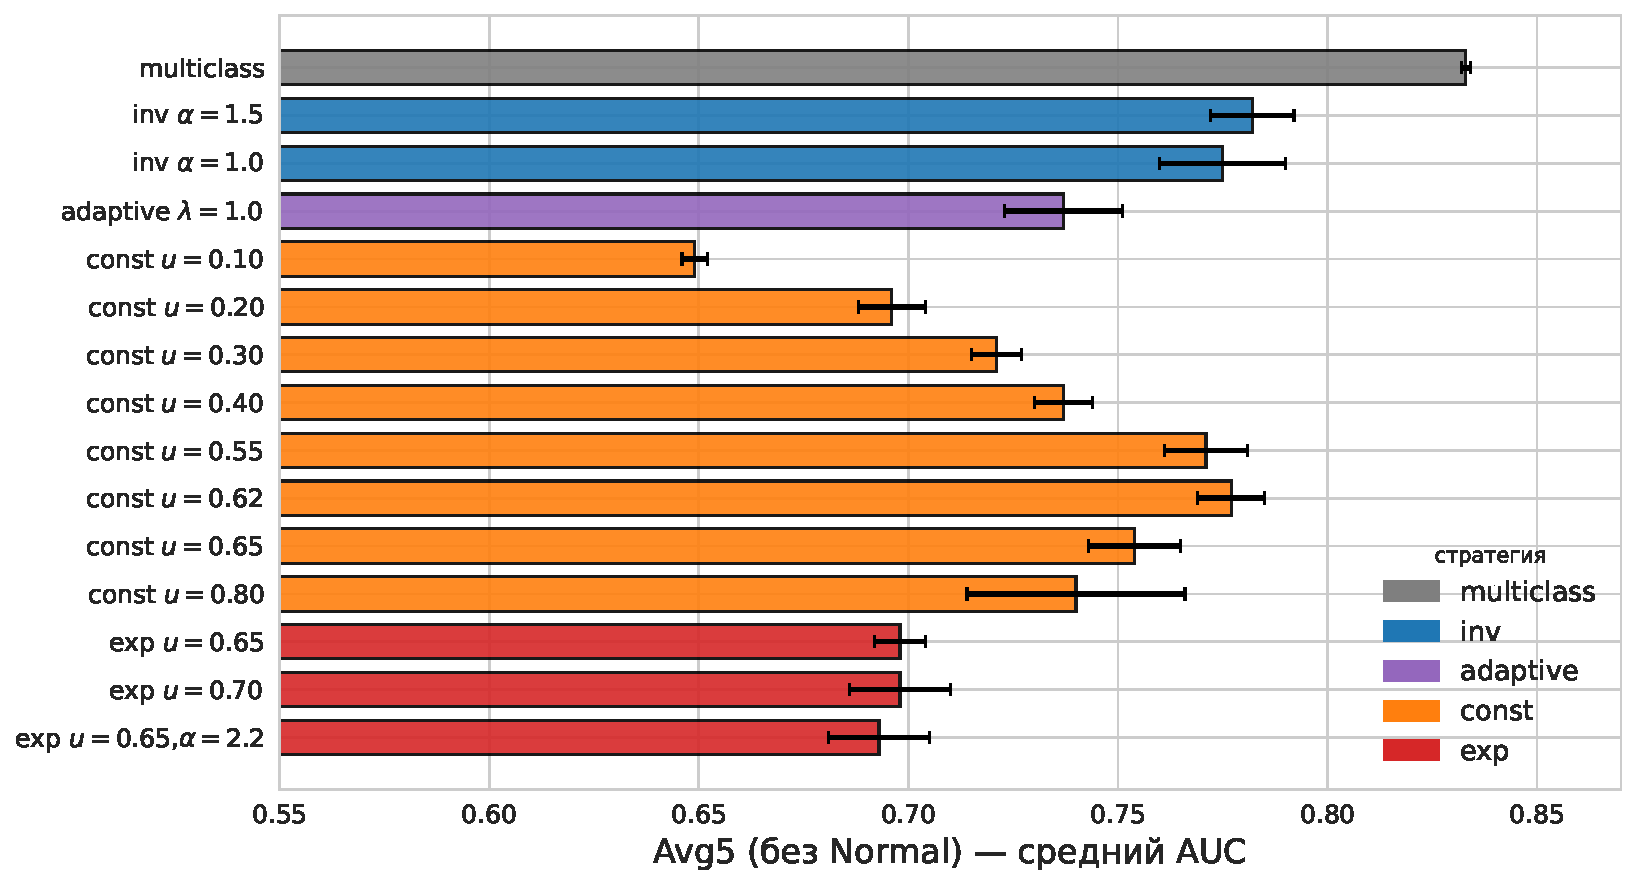
\includegraphics[width=0.92\linewidth]{cxr_summary_bar_avg5.pdf}
    \caption{Сводное сравнение стратегий $u_t$ по метрике Avg5 (средний AUC по пяти болезням без класса <<норма>>). Обозначения те же, что на Рис.~\ref{fig:cxr_summary_avg6}.}
    \label{fig:cxr_summary_avg5}
\end{figure}

\paragraph{Зависимость от параметра $u$ в $\texttt{const}$.}
Финальное качество $\texttt{const}$ имеет максимум около $u = 0{,}62$ (Рис.~\ref{fig:cxr_none_sweep}). При малых $u$ модель практически не видит новые снимки, при больших $u$ повторение не успевает защитить старые задачи.

\begin{figure}[h!]
    \centering
    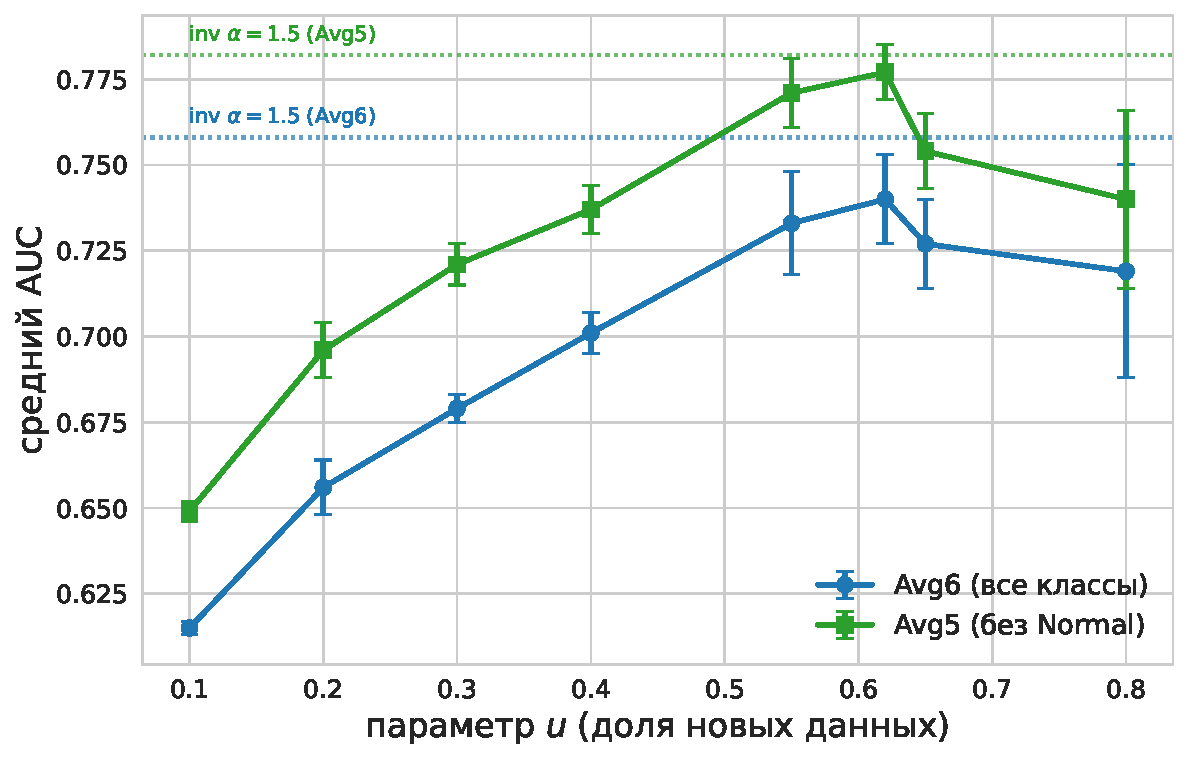
\includegraphics[width=0.75\linewidth]{cxr_none_sweep.pdf}
    \caption{Расписание $\texttt{const}$: зависимость Avg6 и Avg5 от параметра $u$. Пунктир обозначает уровни Avg6 и Avg5 для $\texttt{inv}$ с $\alpha = 1{,}5$.}
    \label{fig:cxr_none_sweep}
\end{figure}

\paragraph{Зависимость от параметра $\lambda$ в $\texttt{adaptive}$.}
Качество $\texttt{adaptive}$ слабо зависит от $\lambda$ в диапазоне $[0{,}5; 1{,}5]$ и не превышает $0{,}74$ по Avg6 (Рис.~\ref{fig:cxr_adaptive_lambda}). Лучший $\lambda = 1$ остается ниже уровня $\texttt{inv}$.

\begin{figure}[h!]
    \centering
    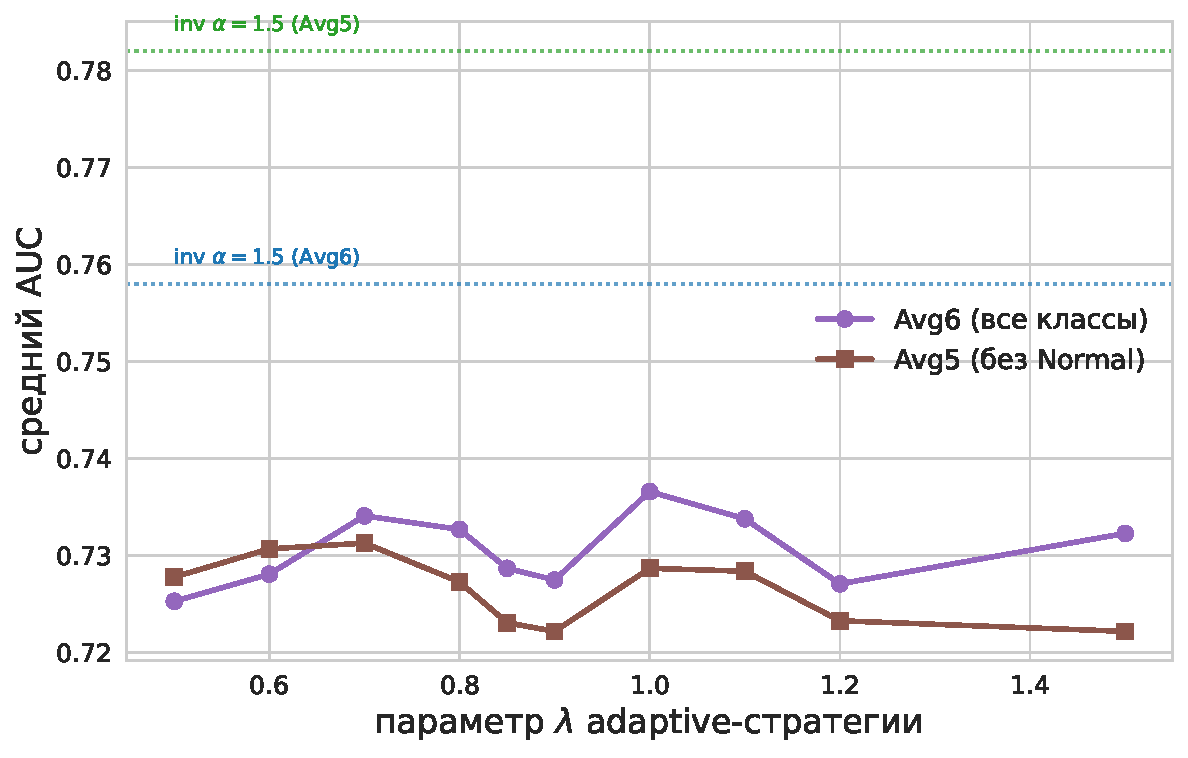
\includegraphics[width=0.75\linewidth]{cxr_adaptive_lambda.pdf}
    \caption{Расписание $\texttt{adaptive}$: зависимость Avg6 и Avg5 от параметра $\lambda$. Пунктир обозначает уровни $\texttt{inv}$ с $\alpha = 1{,}5$.}
    \label{fig:cxr_adaptive_lambda}
\end{figure}

\paragraph{Сравнение с совместным обучением по классам.}
На Рис.~\ref{fig:cxr_per_disease} приведено покомпонентное сравнение лучшего $\texttt{inv}$ с совместным обучением. Наибольший разрыв на Consolidation ($0{,}080$), наименьший на Edema ($0{,}015$), остальные в диапазоне $0{,}04$--$0{,}08$.

\begin{figure}[h!]
    \centering
    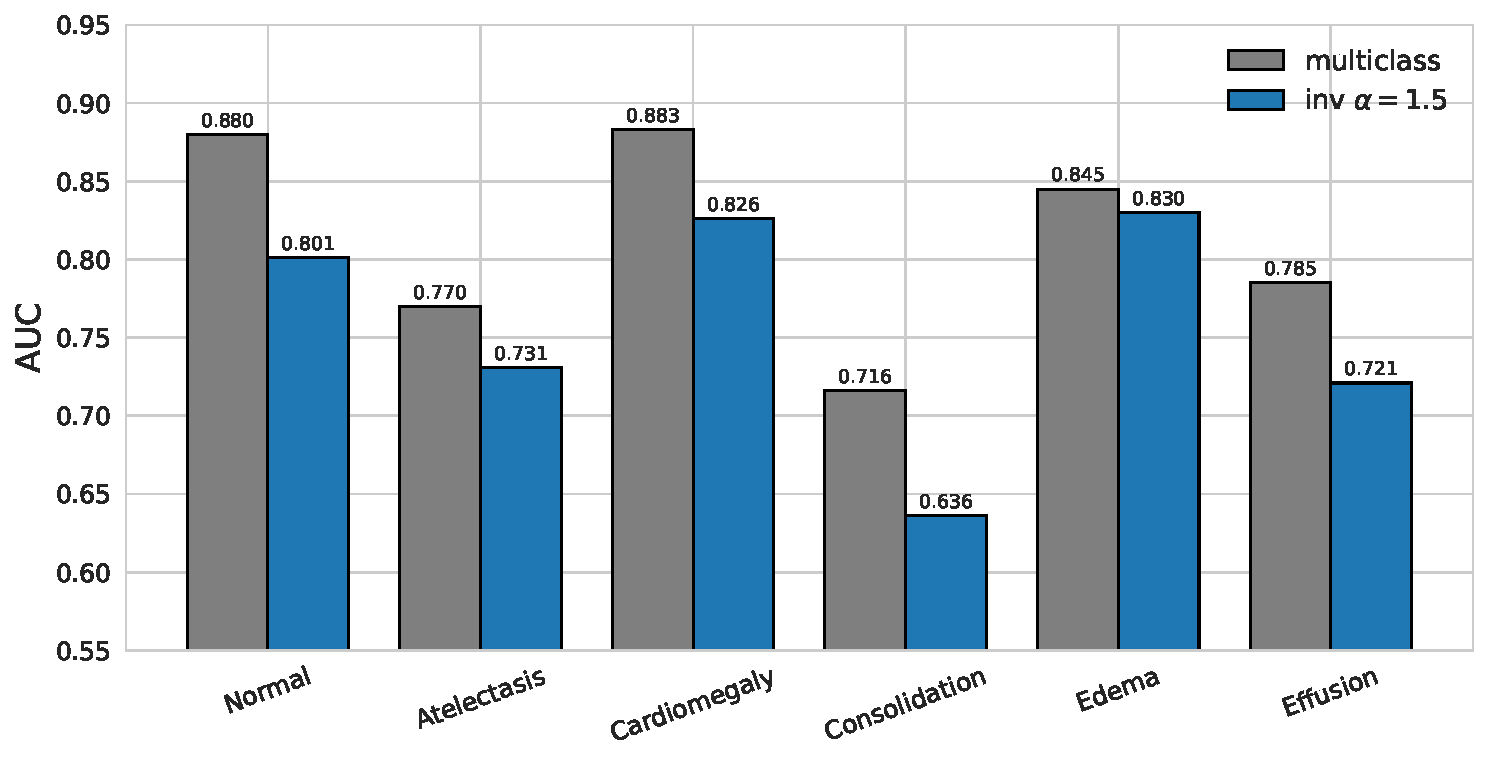
\includegraphics[width=0.82\linewidth]{cxr_per_disease.pdf}
    \caption{Покомпонентное сравнение AUC между $\texttt{multiclass}$ ориентиром и лучшим расписанием $\texttt{inv}$ с $\alpha = 1{,}5$. Усреднение по пяти запускам.}
    \label{fig:cxr_per_disease}
\end{figure}

\paragraph{Динамика AUC по блокам.}
Рис.~\ref{fig:cxr_auc_trajectory} показывает изменение AUC каждой болезни по ходу прохождения блоков для $\texttt{inv}$ с $\alpha = 1{,}5$. На блоке $0$ модель обучена только на классе <<норма>>, AUC по остальным классам близок к $0{,}5$. Каждый следующий блок повышает AUC соответствующей болезни и удерживает уже выученные классы около достигнутого уровня без катастрофических потерь.

\begin{figure}[h!]
    \centering
    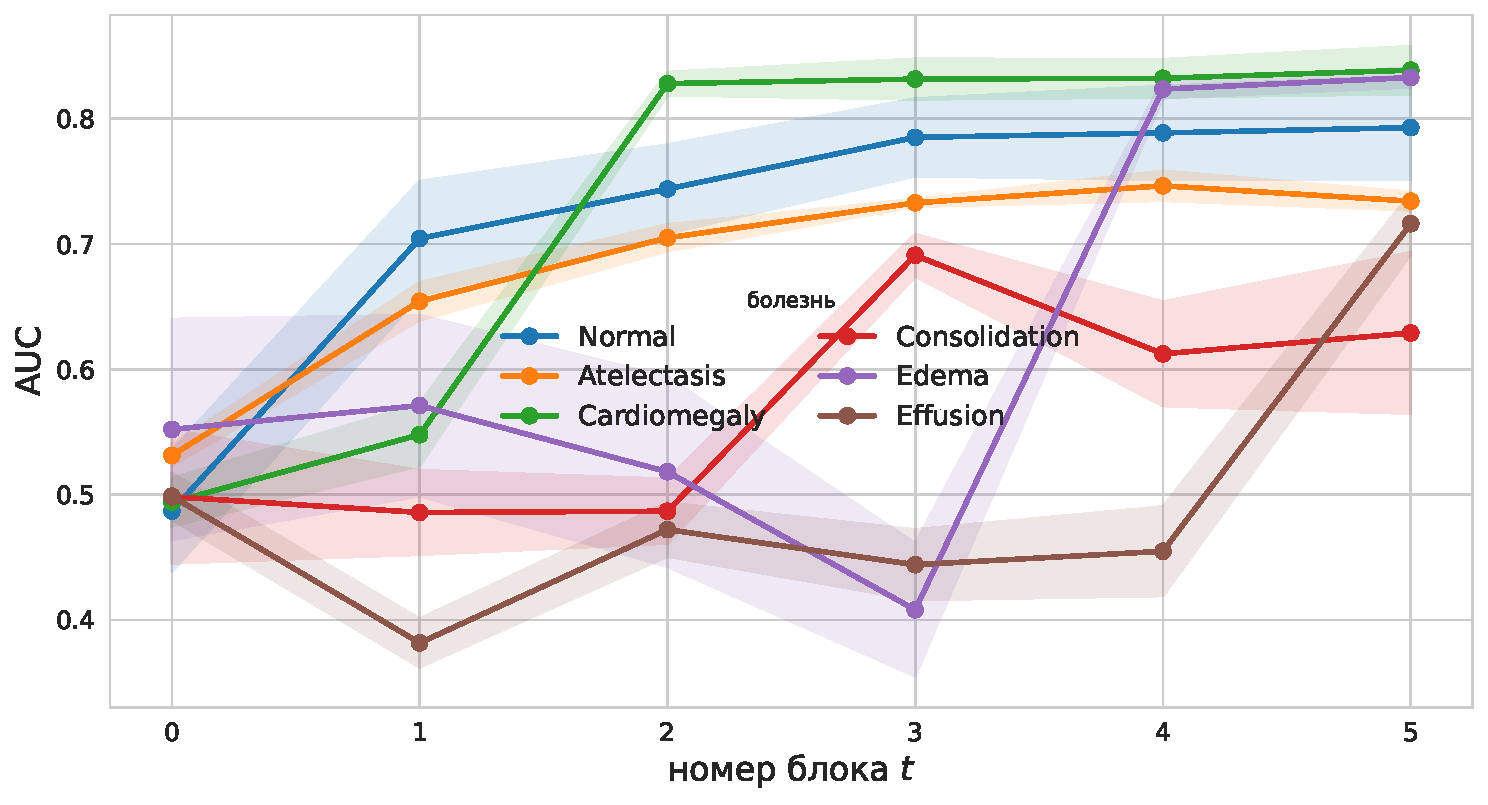
\includegraphics[width=0.82\linewidth]{cxr_auc_trajectory.pdf}
    \caption{Эволюция AUC каждой из шести болезней по блокам обучения для расписания $\texttt{inv}$ с $\alpha = 1{,}5$. Заливка показывает стандартное отклонение по трем запускам.}
    \label{fig:cxr_auc_trajectory}
\end{figure}

\paragraph{Обсуждение.}
На реальном датасете теория Generative Replay воспроизводится в той же качественной картине, что и на синтетике. Расписание $\texttt{inv}$ с $\alpha = 1{,}5$ устойчиво лучше остальных и уступает совместному обучению на $5{,}5$ процентного пункта по Avg6 и на $5{,}1$ по Avg5. Ни $\texttt{const}$, ни $\texttt{adaptive}$ при переборе гиперпараметров до этого уровня не дотягиваются. Выбор расписания через равномерные веса задач (Утверждение~\ref{prop:inverse_gr}) переносится с квадратичных моделей на нелинейные глубокие сети.

Динамика AUC по блокам соответствует ограниченному забыванию: после первого появления каждого класса модель удерживает AUC около достигнутого уровня, что отвечает поведению $u_t = \alpha/(t+1)$ из Теоремы~\ref{thm:avg_error_gr}. Адаптивная стратегия~\eqref{eq:adaptive_u} показывает потенциал, но уступает $\texttt{inv}$, что согласуется с выводом подраздела~\ref{sec:gr} о направлении будущей работы.

% =====================================================================
% Заключение
% =====================================================================
\newpage
\cleardoublepage
\phantomsection
\addcontentsline{toc}{section}{Заключение}
\section*{Заключение}

В работе предложена постановка задачи оптимального управления для систем машинного обучения со скрытой петлей обратной связи. Состояние системы описывается парой $(f_t, h_t)$, оператор эволюции разделен на оператор обучения $\bH_t$ и оператор реакции среды $\bP_t$, а условие $g(f_t, h_{t+1}) \le 0$ задает требования к сохранению петли и работоспособности системы. Постановка применена к двум прикладным сюжетам.

На задаче прогнозирования цен показано, что наивная жадная стратегия по локальной метрике приводит к оттоку пользователей и в пределе разрушает систему. Аккуратное условие $g$ с зависимостью от наблюдаемой выборки восстанавливает работоспособный режим без потери качества предсказания.

Для метода Generative Replay в задаче непрерывного обучения получены достаточные условия допустимости управления через липшицевость потерь и через устойчивость алгоритма обучения к замене одного примера, верхняя оценка средней ошибки модели для произвольного расписания, а также обратная задача восстановления расписания по целевым весам задач с явной формулой $u_t = \alpha_{t+1}/S_{t+1}$. В квадратичном приближении функции потерь выведена замкнутая форма шага Generative Replay, спектральная оценка средней ошибки и безусловная оценка $\bar\varepsilon^* + LD^2/2$. При одинаковых гессианах задач и независимых случайных оптимумах получено разложение средней ошибки на компоненты смещения и дисперсии, а условия сходимости в среднем квадратичном эквивалентны классическим условиям Роббинса-Монро.

Все теоретические результаты проверены экспериментально на синтетических задачах и на реальном датасете NIH ChestX-Ray. Расписание $u_t = 1{,}5/(t+1)$ для последовательной классификации пяти заболеваний поверх класса <<норма>> уступает совместному многоклассовому обучению на $5{,}5$ процентного пункта по средней метрике AUC.

Направления дальнейших исследований. Адаптивное расписание~\eqref{eq:adaptive_u} из подраздела~\ref{sec:gr} в текущем виде уступает $\texttt{inv}$ на реальном датасете. Получение теоретически обоснованной формулы $u_t^*$ через локальную геометрию задачи остается открытой задачей. Спектральная теория получена в режиме идеального генератора $\overline{\cE}_t = 0$. Включение в анализ конечной точности генератора и количественная оценка $\overline{\cE}_t$ через число изученных задач позволили бы получить замкнутые оценки финальной ошибки в режиме длинного потока. Наконец, перенос подхода на онлайн-обучение, где новая задача не имеет фиксированного носителя, а распределение признаков меняется непрерывно, представляет отдельный интерес.

% =====================================================================
% Литература
% =====================================================================
\newpage
\bibliographystyle{unsrtnat}
\bibliography{references}

% =====================================================================
% Приложение
% =====================================================================
\newcounter{appthm}

\newpage
\cleardoublepage
\phantomsection
\addcontentsline{toc}{section}{Приложение А. Непустота множества допустимых управлений}
\section*{Приложение А. Непустота множества допустимых управлений}

В этом приложении приведено полное доказательство Утверждения~\ref{prop:nonempty} из подраздела~\ref{sec:problem_statement} о непустоте множества допустимых управлений на каждом шаге.

\setcounter{appthm}{0}
\renewcommand{\theappthm}{А.\arabic{appthm}}

\refstepcounter{appthm}
\subsection*{\theappthm. Доказательство Утверждения~\ref{prop:nonempty}}\label{app:proof_nonempty}

Применим индукцию по $t$. На нулевом шаге по Предположению~\ref{ass:init} верно $g(f_0, h_0) \le 0$. При $u_0 = 0$ из первого условия утверждения следует $h_1 = h_0$, поэтому $g(f_0, h_1) = g(f_0, h_0) \le 0$, и управление допустимо. Шаг индукции. Пусть $g(f_t, h_t) \le 0$. При $u_t = 0$ снова $h_{t+1} = h_t$, откуда $g(f_t, h_{t+1}) = g(f_t, h_t) \le 0$. Состояние следующего шага есть $f_{t+1} = \bP_t(f_t, h_{t+1})$, и по второму условию утверждения $g(f_{t+1}, h_t) \le 0$. Из $h_{t+1} = h_t$ получаем $g(f_{t+1}, h_{t+1}) \le 0$, что и требовалось.\hfill$\square$

\newpage
\cleardoublepage
\phantomsection
\addcontentsline{toc}{section}{Приложение Б. Достаточные условия допустимости управления}
\section*{Приложение Б. Достаточные условия допустимости управления}

В этом приложении приведены полные доказательства результатов из подраздела~\ref{sec:gr} о достаточных условиях допустимости управления.

\setcounter{appthm}{0}
\renewcommand{\theappthm}{Б.\arabic{appthm}}

\refstepcounter{appthm}
\subsection*{\theappthm. Доказательство Теоремы~\ref{thm:adm_lipschitz}}\label{app:proof_adm_lipschitz}

Требуется показать, что при $u_t \in (0, 1)$ из условий
\[
    \cL_{t+1}(\btheta^{t+1}) \le \frac{\varepsilon_t}{2 u_t}, \qquad d(\btheta^{t+1}, \btheta^t) \le \frac{\varepsilon_t}{2(1 - u_t) L_{\text{loss}}}
\]
следует неравенство $\cL^*_t(u_t) \le \varepsilon_t$, то есть $\varepsilon_t$-допустимость управления.

\paragraph{Шаг 1. Структура обучающего функционала.} По определению Generative Replay
\[
    \cL^*_t(u_t) = \min_{\btheta} \bigl[u_t \cL_{t+1}(\btheta) + (1 - u_t) R_t(\btheta)\bigr],
\]
где $R_t(\btheta) = \bbE_{\bx \sim G_t}\bigl[\cL\bigl(m_{\btheta}(\bx), m_{\btheta^t}(\bx)\bigr)\bigr]$ обозначает функционал повторения с самодистилляцией. Подставляя $\btheta = \btheta^{t+1}$ из условия теоремы, получаем верхнюю оценку
\[
    \cL^*_t(u_t) \le u_t \cL_{t+1}(\btheta^{t+1}) + (1 - u_t) R_t(\btheta^{t+1}).
\]

\paragraph{Шаг 2. Оценка слагаемого повторения через Lipschitz.} Будем считать, что функция потерь является функцией расхождения, $\cL(z, z) = 0$ для всех $z$. Это свойство выполнено для среднеквадратичной потери, кросс-энтропии и расстояния Кульбака-Лейблера. По Предположению~\ref{ass:lipschitz_gr}, применяя разностную оценку к парам $(\btheta^{t+1}, m_{\btheta^t}(\bx))$ и $(\btheta^t, m_{\btheta^t}(\bx))$ и учитывая $\cL(m_{\btheta^t}(\bx), m_{\btheta^t}(\bx)) = 0$, получаем
\[
    \cL\bigl(m_{\btheta^{t+1}}(\bx), m_{\btheta^t}(\bx)\bigr) \le L_{\text{loss}}\cdot d(\btheta^{t+1}, \btheta^t).
\]
Усредняя по $\bx \sim G_t$, получаем
\[
    R_t(\btheta^{t+1}) \le L_{\text{loss}}\cdot d(\btheta^{t+1}, \btheta^t).
\]

\paragraph{Шаг 3. Сборка.} Подставляя обе оценки из условия теоремы:
\[
    \cL^*_t(u_t) \le u_t \cdot \frac{\varepsilon_t}{2 u_t} + (1 - u_t) \cdot L_{\text{loss}} \cdot \frac{\varepsilon_t}{2(1 - u_t) L_{\text{loss}}} = \frac{\varepsilon_t}{2} + \frac{\varepsilon_t}{2} = \varepsilon_t.
\]
Управление $u_t$ удовлетворяет условию $\varepsilon_t$-допустимости.\hfill$\square$

\refstepcounter{appthm}
\subsection*{\theappthm. Доказательство Леммы~\ref{lem:k_replace_gr}}\label{app:proof_k_replace}

Построим цепочку выборок $S = S^{(0)}, S^{(1)}, \ldots, S^{(k)} = S'$, в которой соседние выборки $S^{(i-1)}$ и $S^{(i)}$ отличаются ровно в одной позиции. Такая цепочка существует, поскольку $S$ и $S'$ отличаются не более чем в $k$ позициях, и различающиеся элементы можно заменять последовательно по одному.

По Определению~\ref{def:beta_stab_gr} для каждой пары соседних выборок
\[
    \sup_z \bigl|\cL(\bH_t(S^{(i-1)}), z) - \cL(\bH_t(S^{(i)}), z)\bigr| \le \beta_m.
\]
По неравенству треугольника, накопленному вдоль цепочки длины $k$,
\[
    \sup_z \bigl|\cL(\bH_t(S), z) - \cL(\bH_t(S'), z)\bigr| \le \sum_{i=1}^k \beta_m = k \beta_m.
\]
\hfill$\square$

\refstepcounter{appthm}
\subsection*{\theappthm. Доказательство Теоремы~\ref{thm:adm_stability}}\label{app:proof_adm_stability}

\paragraph{Шаг 1. Стартовая точка.} Обозначим выборку, отвечающую управлению $u$, через $S(u)$: $u m$ объектов новой задачи $D_{t+1}$ и $(1 - u) m$ объектов выборки повторения $\widetilde D_t$. Внутренняя оптимизация выдает веса $\btheta^{t+1}(u) = \bH_t(S(u))$. Считаем $\cL(z, z) = 0$, как в Шаге 2 доказательства Теоремы~\ref{thm:adm_lipschitz}.

При $u = 0$ по условию $\btheta^{t+1}(0) = \btheta^t$. Метки в $\widetilde D_t$ порождены текущей моделью $m_{\btheta^t}$ через самодистилляцию, поэтому на этих объектах
\[
    \cL\bigl(\btheta^{t+1}(0), \widetilde D_t\bigr) = \bbE_{\bx \sim G_t} \cL\bigl(m_{\btheta^t}(\bx), m_{\btheta^t}(\bx)\bigr) = 0.
\]

\paragraph{Шаг 2. Сравнение через устойчивость.} Выборки $S(u_t)$ и $S(0)$ отличаются не более чем в $k_t = u_t m$ позициях: ровно тех, где объекты из $\widetilde D_t$ заменены на объекты новой задачи. По Лемме~\ref{lem:k_replace_gr} и стабильности $\beta_m$:
\[
    \cL\bigl(\btheta^{t+1}(u_t), \widetilde D_t\bigr) \le \cL\bigl(\btheta^{t+1}(0), \widetilde D_t\bigr) + u_t m \beta_m = u_t m \beta_m.
\]

\paragraph{Шаг 3. Сборка.} По определению обучающего функционала и условиям теоремы:
\[
    \cL^*_t(u_t) \le u_t \cL_{t+1}\bigl(\btheta^{t+1}(u_t)\bigr) + (1 - u_t) \cL\bigl(\btheta^{t+1}(u_t), \widetilde D_t\bigr) \le u_t \cdot \frac{\varepsilon_t}{2 u_t} + (1 - u_t) \cdot u_t m \beta_m.
\]
Подставляя $u_t m \beta_m \le \varepsilon_t / (2(1 - u_t))$:
\[
    \cL^*_t(u_t) \le \frac{\varepsilon_t}{2} + (1 - u_t) \cdot \frac{\varepsilon_t}{2(1 - u_t)} = \varepsilon_t.
\]
\hfill$\square$

\newpage
\cleardoublepage
\phantomsection
\addcontentsline{toc}{section}{Приложение В. Верхняя оценка средней ошибки и обратная задача}
\section*{Приложение В. Верхняя оценка средней ошибки и обратная задача}

В этом приложении приведены полные доказательства результатов из подраздела~\ref{sec:gr} о верхней оценке средней ошибки модели и об обратной задаче восстановления расписания.

\setcounter{appthm}{0}
\renewcommand{\theappthm}{В.\arabic{appthm}}

\refstepcounter{appthm}
\subsection*{\theappthm. Доказательство Леммы~\ref{lem:weights_gr}}\label{app:proof_weights}

\paragraph{Шаг 1. Неотрицательность.} Каждое $w_{s, t+1}$ есть произведение неотрицательных множителей: $u_{s-1} \ge 0$ и $(1 - u_r) \ge 0$ при $u_r \in [0, 1]$. Все веса неотрицательны.

\paragraph{Шаг 2. Тождество $u_{s-1} p_s = p_s - p_{s-1}$.} Положим $p_s = \prod_{r=s}^{t}(1 - u_r)$ при $s \le t$ и $p_{t+1} = 1$. Имеем
\[
    p_{s-1} = (1 - u_{s-1}) p_s = p_s - u_{s-1} p_s,
\]
откуда $u_{s-1} p_s = p_s - p_{s-1}$.

\paragraph{Шаг 3. Телескопическое суммирование.} По определению весов $w_{1, t+1} = p_1$, а $w_{s, t+1} = u_{s-1} p_s = p_s - p_{s-1}$ при $s \ge 2$. Тогда
\[
    \sum_{s=1}^{t+1} w_{s, t+1} = p_1 + \sum_{s=2}^{t+1}(p_s - p_{s-1}) = p_1 + (p_{t+1} - p_1) = p_{t+1} = 1.
\]
\hfill$\square$

\refstepcounter{appthm}
\subsection*{\theappthm. Доказательство Леммы~\ref{lem:triangle_gr}}\label{app:proof_triangle}

\paragraph{Шаг 1. Неравенство треугольника на одном объекте.} По Предположению~\ref{ass:triangle_gr} для любых $\btheta^{t+1}, \btheta^t$ и любого объекта $(\bx, y)$
\[
    \cL(m_{\btheta^{t+1}}(\bx), y) \le \cL(m_{\btheta^{t+1}}(\bx), m_{\btheta^t}(\bx)) + \cL(m_{\btheta^t}(\bx), y).
\]
Беря математическое ожидание по $(\bx, y) \sim D_s$,
\begin{equation}
    \cL_s(\btheta^{t+1}) \le \bbE_{\bx \sim p_s}\bigl[\cL(m_{\btheta^{t+1}}(\bx), m_{\btheta^t}(\bx))\bigr] + \cL_s(\btheta^t).
    \label{eq:app_triangle_one_step}
\end{equation}

\paragraph{Шаг 2. Замена истинной плотности признаков на генератор.} Первое слагаемое в~\eqref{eq:app_triangle_one_step} зависит от $\bx$ только через распределение признаков задачи $D_s$. Запишем его как интеграл и добавим и вычтем плотность генератора $p_{G_t}$:
\begin{align*}
    \int \cL(m_{\btheta^{t+1}}(\bx), m_{\btheta^t}(\bx)) p_s(\bx)\, d\bx &= \int \cL(m_{\btheta^{t+1}}(\bx), m_{\btheta^t}(\bx)) p_{G_t}(\bx)\, d\bx \\
    &\quad + \int \cL(m_{\btheta^{t+1}}(\bx), m_{\btheta^t}(\bx))\bigl(p_s(\bx) - p_{G_t}(\bx)\bigr)\, d\bx.
\end{align*}
Первый интеграл равен $\bbE_{\bx \sim G_t}[\cL(m_{\btheta^{t+1}}(\bx), m_{\btheta^t}(\bx))]$.

\paragraph{Шаг 3. Оценка второго интеграла.} Как и в Шаге 2 доказательства Теоремы~\ref{thm:adm_lipschitz}, считаем $\cL(z, z) = 0$. По Предположению~\ref{ass:lipschitz_gr} с учетом $\cL(m_{\btheta^t}(\bx), m_{\btheta^t}(\bx)) = 0$ для всех $\bx$ выполнено
\[
    \cL(m_{\btheta^{t+1}}(\bx), m_{\btheta^t}(\bx)) \le L_{\text{loss}}\cdot d(\btheta^{t+1}, \btheta^t).
\]
Обозначим $\Delta p(\bx) = p_s(\bx) - p_{G_t}(\bx)$. По неравенству $|\int f \Delta p|\le \sup|f| \cdot \int|\Delta p|$ и оценке Шага~3 получаем
\begin{align*}
    \biggl|\int \cL(m_{\btheta^{t+1}}(\bx), m_{\btheta^t}(\bx))\,\Delta p(\bx)\, d\bx\biggr|
    &\le L_{\text{loss}}\cdot d(\btheta^{t+1}, \btheta^t)\cdot \int |\Delta p(\bx)|\, d\bx \\
    &= \cE_{\mathrm{gen}}(s, t).
\end{align*}

\paragraph{Шаг 4. Сборка.} Объединяя три шага:
\[
    \cL_s(\btheta^{t+1}) \le \bbE_{\bx \sim G_t}\bigl[\cL(m_{\btheta^{t+1}}(\bx), m_{\btheta^t}(\bx))\bigr] + \cL_s(\btheta^t) + \cE_{\mathrm{gen}}(s, t).
\]
\hfill$\square$

\refstepcounter{appthm}
\subsection*{\theappthm. Доказательство Теоремы~\ref{thm:avg_error_gr}}\label{app:proof_avg_error}

Обозначим через $\cL^{(w)}_{t+1} = \sum_{s=1}^{t+1} w_{s, t+1} \cL_s(\btheta^{t+1})$ взвешенную среднюю ошибку модели после шага $t$, через $R_t(\btheta) = \bbE_{\bx \sim G_t}\bigl[\cL\bigl(m_{\btheta}(\bx), m_{\btheta^t}(\bx)\bigr)\bigr]$ функционал повторения. Обучающий функционал из определения GR имеет вид
\begin{equation}
    \cL^*_t(u_t) = u_t \cL_{t+1}(\btheta^{t+1}) + (1 - u_t) R_t(\btheta^{t+1}),
    \label{eq:app_Lstar}
\end{equation}
а по условию $\varepsilon_t$-допустимости $\cL^*_t(u_t) \le \varepsilon_t$. Агрегированная ошибка генератора определяется как $\overline{\mathcal E}_t = L_{\text{loss}}\, d(\btheta^{t+1}, \btheta^t) \sum_{s=1}^t w_{s, t}\, \cE_{\mathrm{gen}}(s, t)$.

\paragraph{Шаг 1. Расщепление весов.} Из Определения~\ref{def:weights_gr} напрямую следует
\begin{align*}
    w_{1, t+1} &= \prod_{r=1}^{t}(1 - u_r) = (1 - u_t)\, w_{1, t}, \\
    w_{s, t+1} &= u_{s-1}\prod_{r=s}^{t}(1 - u_r) = (1 - u_t)\, w_{s, t}, \quad 2 \le s \le t, \\
    w_{t+1, t+1} &= u_t.
\end{align*}
Подставляя в определение $\cL^{(w)}_{t+1}$, получаем
\begin{equation}
    \cL^{(w)}_{t+1} = (1 - u_t)\sum_{s=1}^{t} w_{s, t} \cL_s(\btheta^{t+1}) + u_t \cL_{t+1}(\btheta^{t+1}).
    \label{eq:app_recur_L}
\end{equation}

\paragraph{Шаг 2. Применение Леммы~\ref{lem:triangle_gr} к каждой задаче.} Для каждого $s \le t$ Лемма~\ref{lem:triangle_gr} дает
\[
    \cL_s(\btheta^{t+1}) \le R_t(\btheta^{t+1}) + \cL_s(\btheta^t) + {L_{\text{loss}}\, d(\btheta^{t+1}, \btheta^t)\,} \cE_{\mathrm{gen}}(s, t),
\]
где $R_t(\btheta^{t+1}) = \bbE_{\bx \sim G_t}\bigl[\cL(m_{\btheta^{t+1}}(\bx), m_{\btheta^t}(\bx))\bigr]$ и множитель $L_{\text{loss}}\, d(\btheta^{t+1}, \btheta^t)$ не зависят от $s$. Усредняя с весами $w_{s, t}$ и пользуясь $\sum_{s=1}^t w_{s, t} = 1$ (Лемма~\ref{lem:weights_gr}):
\begin{equation}
    \sum_{s=1}^{t} w_{s, t} \cL_s(\btheta^{t+1}) \le R_t(\btheta^{t+1}) + \cL^{(w)}_t + \overline{\mathcal E}_t,
    \label{eq:app_avg_triangle}
\end{equation}
где $\cL^{(w)}_t = \sum_s w_{s, t} \cL_s(\btheta^t)$ обозначает взвешенную среднюю ошибку на прошлом шаге.

\paragraph{Шаг 3. Сборка рекуррентной оценки.} Подставляя~\eqref{eq:app_avg_triangle} в~\eqref{eq:app_recur_L}:
\begin{align*}
    \cL^{(w)}_{t+1} &\le (1 - u_t)\bigl[R_t(\btheta^{t+1}) + \cL^{(w)}_t + \overline{\mathcal E}_t\bigr] + u_t \cL_{t+1}(\btheta^{t+1}) \\
    &= \bigl[u_t \cL_{t+1}(\btheta^{t+1}) + (1 - u_t) R_t(\btheta^{t+1})\bigr] + (1 - u_t)\cL^{(w)}_t + (1 - u_t)\overline{\mathcal E}_t \\
    &= \cL^*_t(u_t) + (1 - u_t)\cL^{(w)}_t + (1 - u_t)\overline{\mathcal E}_t.
\end{align*}
По условию $\cL^*_t(u_t) \le \varepsilon_t$, а $(1 - u_t)\overline{\mathcal E}_t \le \overline{\mathcal E}_t$ при $\overline{\mathcal E}_t \ge 0$. Получаем
\[
    \cL^{(w)}_{t+1} \le \varepsilon_t + (1 - u_t)\cL^{(w)}_t + \overline{\mathcal E}_t.
\]

\paragraph{Шаг 4. Разворачивание рекурсии.} Пусть $a_t = \cL^{(w)}_t$, $b_t = \varepsilon_t + \overline{\mathcal E}_t$. Имеем рекурсию $a_{t+1} \le b_t + (1 - u_t) a_t$ с $a_0 = 0$. Индукция по $t$ дает
\[
    a_{t+1} \le \sum_{j=0}^{t}\Bigl(\prod_{r=j+1}^{t}(1 - u_r)\Bigr) b_j.
\]
Раскрывая $b_j = \varepsilon_j + \overline{\mathcal E}_j$ и учитывая $\overline{\mathcal E}_0 = 0$ (на первом шаге задач для повторения нет),
\[
    \cL^{(w)}_{t+1} \le \sum_{j=0}^{t}\Bigl(\prod_{r=j+1}^{t}(1 - u_r)\Bigr)\varepsilon_j + \sum_{j=1}^{t}\Bigl(\prod_{r=j+1}^{t}(1 - u_r)\Bigr) \overline{\mathcal E}_j.
\]
\hfill$\square$

\refstepcounter{appthm}
\subsection*{\theappthm. Доказательство Утверждения~\ref{prop:inverse_gr}}\label{app:proof_inverse}

Требуется показать, что управления $u_t = \alpha_{t+1}/S_{t+1}$ порождают веса $w_{s, T} = \alpha_s$ для всех $s$.

\paragraph{Шаг 1. Стартовое значение.} При $t = 0$ имеем $u_0 = \alpha_1 / S_1 = 1$, так как $S_1 = \alpha_1$.

\paragraph{Шаг 2. Связь $1 - u_t$ и частичных сумм.} При $t \ge 1$ из определения $u_t = \alpha_{t+1}/S_{t+1}$ и $S_{t+1} = S_t + \alpha_{t+1}$:
\[
    1 - u_t = \frac{S_{t+1} - \alpha_{t+1}}{S_{t+1}} = \frac{S_t}{S_{t+1}}.
\]
Тогда
\[
    \prod_{r=s}^{T-1}(1 - u_r) = \prod_{r=s}^{T-1}\frac{S_r}{S_{r+1}} = \frac{S_s \cdot S_{s+1}\cdots S_{T-1}}{S_{s+1}\cdot S_{s+2}\cdots S_T} = \frac{S_s}{S_T} = S_s,
\]
поскольку $S_T = \sum_{s=1}^T \alpha_s = 1$.

\paragraph{Шаг 3. Подстановка в определение весов.} Для $s \ge 2$:
\[
    w_{s, T} = u_{s-1}\prod_{r=s}^{T-1}(1 - u_r) = \frac{\alpha_s}{S_s} \cdot S_s = \alpha_s.
\]
Для $s = 1$ произведение начинается с $r = 1$, поэтому значение $u_0 = 1$ в нем не участвует:
\[
    w_{1, T} = \prod_{r=1}^{T-1}(1 - u_r) = S_1 = \alpha_1.
\]
\hfill$\square$

\newpage
\cleardoublepage
\phantomsection
\addcontentsline{toc}{section}{Приложение Г. Спектральная теория ошибки в квадратичном приближении}
\section*{Приложение Г. Спектральная теория ошибки в квадратичном приближении}

В этом приложении приведены полные доказательства результатов из подраздела~\ref{sec:gr} о замкнутой форме шага Generative Replay, спектральной оценке средней ошибки, условии нулевого конфликта и безусловной оценке $\bar\varepsilon^* + LD^2/2$.

\setcounter{appthm}{0}
\renewcommand{\theappthm}{Г.\arabic{appthm}}

\refstepcounter{appthm}
\subsection*{\theappthm. Доказательство Леммы~\ref{lem:gr_step}}\label{app:proof_gr_step}

В условиях Предположения~\ref{ass:quad_gr} обучающий функционал имеет вид
\begin{equation}
    \cL_{\text{train}}(\btheta) = u_t\Bigl[\varepsilon^*_{t+1} + \tfrac{1}{2}(\btheta - \btheta^*_{t+1})^\top H_{t+1}(\btheta - \btheta^*_{t+1})\Bigr] + (1 - u_t)\cdot \tfrac{1}{2}(\btheta - \btheta^t)^\top \Sigma_t(\btheta - \btheta^t).
    \label{eq:app_train_quad}
\end{equation}
Это сумма двух квадратичных форм с центрами $\btheta^*_{t+1}$ и $\btheta^t$ и положительно полуопределенными матрицами $H_{t+1}$ и $\Sigma_t$.

\paragraph{Шаг 1. Градиент.} Дифференцируя~\eqref{eq:app_train_quad} по $\btheta$:
\[
    \nabla_{\btheta} \cL_{\text{train}}(\btheta) = u_t H_{t+1}\bigl(\btheta - \btheta^*_{t+1}\bigr) + (1 - u_t)\Sigma_t\bigl(\btheta - \btheta^t\bigr).
\]
Собирая по $\btheta$:
\[
    \nabla_{\btheta} \cL_{\text{train}}(\btheta) = M_t \btheta - b_t,
\]
где $M_t = u_t H_{t+1} + (1 - u_t)\Sigma_t$ и $b_t = u_t H_{t+1}\btheta^*_{t+1} + (1 - u_t)\Sigma_t\btheta^t$.

\paragraph{Шаг 2. Условие минимума.} Матрица $M_t$ положительно полуопределена как линейная комбинация положительно полуопределенных $H_{t+1}$ и $\Sigma_t$ с неотрицательными коэффициентами. При положительно определенном гессиане $H_{t+1}$ и $u_t > 0$ матрица $M_t$ обратима. Точка минимума находится из $\nabla \cL_{\text{train}} = 0$:
\[
    \btheta^{t+1} = M_t^{-1} b_t = M_t^{-1}\bigl[u_t H_{t+1}\btheta^*_{t+1} + (1 - u_t)\Sigma_t\btheta^t\bigr].
\]
\hfill$\square$

\refstepcounter{appthm}
\subsection*{\theappthm. Доказательство Леммы~\ref{lem:gr_delta}}\label{app:proof_gr_delta}

Введем сокращения $A = H_{t+1}$, $S = \Sigma_t$, $\Delta_t = \btheta^*_{t+1} - \btheta^t$. По Лемме~\ref{lem:gr_step} в квадратичном приближении
\begin{equation}
    \btheta^{t+1} = M_t^{-1}\bigl[u_t A \btheta^*_{t+1} + (1 - u_t) S \btheta^t\bigr], \qquad M_t = u_t A + (1 - u_t) S.
    \label{eq:app_step}
\end{equation}

\paragraph{Шаг 1. Подстановка расписания $u_t = 1/(t+1)$.} В этом случае $1 - u_t = t/(t+1)$, поэтому
\[
    M_t = \frac{1}{t+1}\bigl(A + t S\bigr), \qquad K := A + t S, \qquad \btheta^{t+1} = K^{-1}\bigl(A \btheta^*_{t+1} + t S \btheta^t\bigr).
\]

\paragraph{Шаг 2. Отклонения $\btheta^{t+1}$ от точек $\btheta^*_{t+1}$ и $\btheta^t$.} Прямой подсчет:
\begin{align*}
    \btheta^{t+1} - \btheta^*_{t+1} &= K^{-1}\bigl(A \btheta^*_{t+1} + t S \btheta^t - K \btheta^*_{t+1}\bigr) = K^{-1}\cdot tS\bigl(\btheta^t - \btheta^*_{t+1}\bigr) = -t K^{-1} S \Delta_t, \\
    \btheta^{t+1} - \btheta^t &= K^{-1}\bigl(A \btheta^*_{t+1} + t S \btheta^t - K \btheta^t\bigr) = K^{-1} A \bigl(\btheta^*_{t+1} - \btheta^t\bigr) = K^{-1} A \Delta_t.
\end{align*}

\paragraph{Шаг 3. Значения функционалов в точке $\btheta^{t+1}$.} По Предположению~\ref{ass:quad_gr}:
\begin{align*}
    \cL_{t+1}(\btheta^{t+1}) &= \varepsilon^*_{t+1} + \tfrac{1}{2}\bigl(\btheta^{t+1} - \btheta^*_{t+1}\bigr)^\top A \bigl(\btheta^{t+1} - \btheta^*_{t+1}\bigr) \\
    &= \varepsilon^*_{t+1} + \tfrac{t^2}{2}\Delta_t^\top S K^{-1} A K^{-1} S \Delta_t, \\
    R_t(\btheta^{t+1}) &= \tfrac{1}{2}\bigl(\btheta^{t+1} - \btheta^t\bigr)^\top S \bigl(\btheta^{t+1} - \btheta^t\bigr) = \tfrac{1}{2}\Delta_t^\top A K^{-1} S K^{-1} A \Delta_t.
\end{align*}
Подставляя в~\eqref{eq:app_Lstar}:
\begin{align}
    \cL^*_t(u_t) &= \frac{1}{t+1}\Bigl[\varepsilon^*_{t+1} + \tfrac{t^2}{2}\Delta_t^\top S K^{-1} A K^{-1} S \Delta_t\Bigr] + \frac{t}{t+1}\cdot \tfrac{1}{2}\Delta_t^\top A K^{-1} S K^{-1} A \Delta_t \notag \\
    &= \frac{\varepsilon^*_{t+1}}{t+1} + \frac{t}{2(t+1)}\,\Delta_t^\top \bigl[t S K^{-1} A K^{-1} S + A K^{-1} S K^{-1} A\bigr]\Delta_t.
    \label{eq:app_Lstar_quad}
\end{align}

\paragraph{Шаг 4. Алгебраическое тождество.} Из определения $K = A + tS$ умножением на $K^{-1}$ справа и слева получаем
\[
    A K^{-1} + t S K^{-1} = I, \qquad K^{-1} A + t K^{-1} S = I,
\]
откуда $S K^{-1} = \tfrac{1}{t}\bigl(I - A K^{-1}\bigr)$ и $K^{-1} S = \tfrac{1}{t}\bigl(I - K^{-1} A\bigr)$. Матрицы $A$, $S$ симметричны, поэтому $K = K^\top$ и $K^{-1} = (K^{-1})^\top$. Прямое умножение дает $S K^{-1} A = \tfrac{1}{t}(A - A K^{-1} A)$, а $A K^{-1} S = (S K^{-1} A)^\top$ совпадает с правой частью по симметрии. Тождество не требует общей собственной базы для $A$ и $S$. Отсюда
\begin{equation}
    A K^{-1} S \;=\; S K^{-1} A \;=\; \tfrac{1}{t}\bigl(A - A K^{-1} A\bigr).
    \label{eq:app_AKS_identity}
\end{equation}
По этим тождествам левая часть~\eqref{eq:app_Lstar_quad} переписывается покомпонентно:
\begin{align*}
    t S K^{-1} A K^{-1} S &= \bigl(I - A K^{-1}\bigr) A K^{-1} S = A K^{-1} S - \tfrac{1}{t}\bigl(A K^{-1} A - A K^{-1} A K^{-1} A\bigr), \\
    A K^{-1} S K^{-1} A &= A K^{-1} \cdot S K^{-1} A = \tfrac{1}{t}\bigl(A K^{-1} A - A K^{-1} A K^{-1} A\bigr).
\end{align*}
При суммировании члены $\tfrac{1}{t}\bigl(A K^{-1} A - A K^{-1} A K^{-1} A\bigr)$ взаимно сокращаются:
\[
    t S K^{-1} A K^{-1} S + A K^{-1} S K^{-1} A = A K^{-1} S = H_{t+1}\bigl(H_{t+1} + t \Sigma_t\bigr)^{-1} \Sigma_t.
\]

\paragraph{Шаг 5. Финальная формула.} Подставляя в~\eqref{eq:app_Lstar_quad}:
\[
    \cL^*_t(u_t) = \frac{\varepsilon^*_{t+1}}{t+1} + \frac{t}{2(t+1)}\,\Delta_t^\top H_{t+1}\bigl(H_{t+1} + t \Sigma_t\bigr)^{-1} \Sigma_t \Delta_t = \frac{\varepsilon^*_{t+1}}{t+1} + \pi_t.
\]
\hfill$\square$

\refstepcounter{appthm}
\subsection*{\theappthm. Доказательство Теоремы~\ref{thm:spectral_gr}}\label{app:proof_spectral_gr}

При расписании $u_t = 1/(t+1)$ веса из Определения~\ref{def:weights_gr} принимают вид $w_{s, T} = 1/T$ для всех $s$. Проверка: $w_{1, T} = \prod_{r=1}^{T-1} r/(r+1) = 1/T$ телескопически, а при $s \ge 2$ имеем $w_{s, T} = \tfrac{1}{s}\prod_{r=s}^{T-1} r/(r+1) = \tfrac{1}{s}\cdot \tfrac{s}{T} = 1/T$. Поэтому $\cL^{(w)}_T = \cL_T = \tfrac{1}{T}\sum_{s=1}^T \cL_s(\btheta^T)$.

При идеальном генераторе $\overline{\mathcal E}_t = 0$. В доказательстве Теоремы~\ref{thm:avg_error_gr} рекурсия Шага~3 до релаксации $\cL^*_t(u_t) \le \varepsilon_t$ имеет вид $\cL^{(w)}_{t+1} \le \cL^*_t(u_t) + (1 - u_t)\cL^{(w)}_t$. При точной внутренней оптимизации подстановка значений $\cL^*_j(u_j)$ из Леммы~\ref{lem:gr_delta} ниже дает более тугую оценку, чем формулировка Теоремы~\ref{thm:avg_error_gr} через $\varepsilon_j$. Разворачивая рекурсию с $\cL^{(w)}_0 = 0$, получаем
\begin{equation}
    \cL_T \le \sum_{j=0}^{T-1}\Bigl(\prod_{r=j+1}^{T-1}(1 - u_r)\Bigr)\cL^*_j(u_j).
    \label{eq:app_unfolded}
\end{equation}

\paragraph{Шаг 1. Произведения $(1-u_r)$ телескопируют.} При $1 - u_r = r/(r+1)$
\[
    \prod_{r=j+1}^{T-1}\frac{r}{r+1} = \frac{(j+1)(j+2)\cdots(T-1)}{(j+2)(j+3)\cdots T} = \frac{j+1}{T}.
\]

\paragraph{Шаг 2. Подстановка из Леммы~\ref{lem:gr_delta}.} Имеем $\cL^*_j(u_j) = \varepsilon^*_{j+1}/(j+1) + \pi_j$. Тогда
\[
    \cL_T \le \sum_{j=0}^{T-1}\frac{j+1}{T}\Bigl[\frac{\varepsilon^*_{j+1}}{j+1} + \pi_j\Bigr] = \frac{1}{T}\sum_{j=0}^{T-1} \varepsilon^*_{j+1} + \frac{1}{T}\sum_{j=0}^{T-1}(j+1)\pi_j = \bar\varepsilon^* + \frac{1}{T}\sum_{t=0}^{T-1}(t+1)\pi_t,
\]
где $\bar\varepsilon^* = \tfrac{1}{T}\sum_{s=1}^T \varepsilon^*_s$, что совпадает с~\eqref{eq:spectral_master_gr}.\hfill$\square$

\refstepcounter{appthm}
\subsection*{\theappthm. Доказательство Следствия~\ref{cor:zero_conflict_gr}}\label{app:proof_zero_conflict}

По Шагу~5 доказательства Леммы~\ref{lem:gr_delta}
\[
    \pi_t = \frac{t}{2(t+1)}\,\Delta_t^\top H_{t+1}\bigl(H_{t+1} + t\Sigma_t\bigr)^{-1} \Sigma_t \Delta_t.
\]
Положим $K = H_{t+1} + t\Sigma_t$ и покажем, что условие $H_{t+1}\Sigma_t = 0$ влечет $H_{t+1} K^{-1}\Sigma_t = 0$. Для произвольного $u$ обозначим $v = K^{-1}\Sigma_t u$. Тогда $K v = \Sigma_t u$, откуда $H_{t+1} v = \Sigma_t u - t\Sigma_t v = \Sigma_t (u - t v)$. По условию $H_{t+1}\Sigma_t = 0$, поэтому $H_{t+1}^2 v = H_{t+1}\Sigma_t (u - t v) = 0$. Для симметричной положительно полуопределенной матрицы равенство $H_{t+1}^2 v = 0$ равносильно $H_{t+1} v = 0$, откуда $H_{t+1} K^{-1}\Sigma_t u = 0$. Поскольку $u$ произвольно, $H_{t+1} K^{-1}\Sigma_t = 0$ и $\pi_t = 0$ для всех $t$.

При $\pi_t = 0$ для всех $t$ из~\eqref{eq:spectral_master_gr} получаем $\cL_T \le \bar\varepsilon^*$. С другой стороны, $\cL_s(\btheta) \ge \varepsilon^*_s$ для любых весов $\btheta$ по Предположению~\ref{ass:quad_gr}, поэтому
\[
    \cL_T = \frac{1}{T}\sum_{s=1}^T \cL_s(\btheta^T) \ge \frac{1}{T}\sum_{s=1}^T \varepsilon^*_s = \bar\varepsilon^*.
\]
Два встречных неравенства дают равенство $\cL_T = \bar\varepsilon^*$.\hfill$\square$

\refstepcounter{appthm}
\subsection*{\theappthm. Доказательство Теоремы~\ref{thm:unconditional_gr}}\label{app:proof_unconditional_gr}

При $t = 0$ множитель $t/(2(t+1))$ в определении $\pi_t$ обращает $\pi_0 = 0$ независимо от структуры $H_1$ и $\Sigma_0$, и оценка $\pi_0 \le LD^2/(2(0+1))$ выполнена тривиально. Пусть далее $t \ge 1$. Положим $K = H_{t+1} + t\Sigma_t$. По Шагу~5 доказательства Леммы~\ref{lem:gr_delta} и тождеству~\eqref{eq:app_AKS_identity} имеем
\[
    H_{t+1} K^{-1}\Sigma_t = \tfrac{1}{t}\bigl(H_{t+1} - H_{t+1} K^{-1} H_{t+1}\bigr),
\]
откуда
\[
    \pi_t = \frac{1}{2(t+1)}\Bigl(\Delta_t^\top H_{t+1}\Delta_t - \Delta_t^\top H_{t+1} K^{-1} H_{t+1}\Delta_t\Bigr).
\]
Второе слагаемое неотрицательно: при $w = H_{t+1}\Delta_t$ имеем $\Delta_t^\top H_{t+1} K^{-1} H_{t+1}\Delta_t = w^\top K^{-1} w \ge 0$, так как $K \succ 0$. Поэтому
\[
    \pi_t \le \frac{1}{2(t+1)}\Delta_t^\top H_{t+1}\Delta_t \le \frac{\|H_{t+1}\|_{\text{op}}\|\Delta_t\|^2}{2(t+1)} \le \frac{L D^2}{2(t+1)}.
\]
Подставляя в~\eqref{eq:spectral_master_gr}, получаем
\[
    \cL_T - \bar\varepsilon^* \le \frac{1}{T}\sum_{t=0}^{T-1}(t+1)\cdot \frac{L D^2}{2(t+1)} = \frac{1}{T}\cdot T \cdot \frac{L D^2}{2} = \frac{L D^2}{2}.
\]
\hfill$\square$

\newpage
\cleardoublepage
\phantomsection
\addcontentsline{toc}{section}{Приложение Д. Bias-variance анализ и связь с классической теорией}
\section*{Приложение Д. Bias-variance анализ и связь с классической теорией}

В этом приложении приведены полные доказательства результатов из подраздела~\ref{sec:gr} о редукции шага Generative Replay к экспоненциальному скользящему среднему, разложении средней ошибки на смещение и дисперсию и условиях сходимости в среднем квадратичном.

\setcounter{appthm}{0}
\renewcommand{\theappthm}{Д.\arabic{appthm}}

\refstepcounter{appthm}
\subsection*{\theappthm. Доказательство Леммы~\ref{lem:gr_ema}}\label{app:proof_gr_ema}

По Предположению~\ref{ass:common_H_gr} все задачи имеют одинаковый гессиан $H_s = H$, а операционный гессиан функционала повторения $\Sigma_t = H$. Подставляя в~\eqref{eq:gr_step}:
\[
    M_t = u_t H + (1 - u_t) H = H.
\]
Матрица $M_t$ совпадает с $H$ и невырождена при положительно определенном $H$, поэтому $M_t^{-1} = H^{-1}$ и $M_t^{-1} H = I$. Подставляя в выражение для шага:
\[
    \btheta^{t+1} = H^{-1}\bigl[u_t H \btheta^*_{t+1} + (1 - u_t) H \btheta^t\bigr] = u_t \btheta^*_{t+1} + (1 - u_t)\btheta^t = (1 - u_t)\btheta^t + u_t \btheta^*_{t+1}.
\]
Шаг GR принимает вид экспоненциального скользящего среднего по последовательности оптимумов задач.\hfill$\square$

\refstepcounter{appthm}
\subsection*{\theappthm. Доказательство Теоремы~\ref{thm:bv_gr}}\label{app:proof_bv_gr}

По Лемме~\ref{lem:gr_ema} при Предположениях~\ref{ass:common_H_gr} и~\ref{ass:iid_targets_gr} шаг GR имеет вид экспоненциального скользящего среднего $\btheta^{t+1} = (1 - u_t)\btheta^t + u_t \btheta^*_{t+1}$. Раскрывая рекурсию с начальным $\btheta^0$,
\begin{equation}
    \btheta^t = \Pi_t \btheta^0 + \sum_{s=0}^{t-1} w_s^{(t)} \btheta^*_{s+1}, \qquad \Pi_t = \prod_{s=0}^{t-1}(1 - u_s), \quad w_s^{(t)} = u_s \prod_{k=s+1}^{t-1}(1 - u_k).
    \label{eq:app_unrolled}
\end{equation}

\paragraph{Шаг 1. Нормировка весов.} Покажем, что $\Pi_t + \sum_{s=0}^{t-1} w_s^{(t)} = 1$. База: $\Pi_1 + w_0^{(1)} = (1 - u_0) + u_0 = 1$. Переход: при справедливости равенства для $t$
\[
    \Pi_{t+1} + \sum_{s=0}^{t} w_s^{(t+1)} = (1 - u_t)\Pi_t + (1 - u_t)\sum_{s=0}^{t-1} w_s^{(t)} + u_t = (1 - u_t)\cdot 1 + u_t = 1.
\]
В частности, $\sum_{s=0}^{t-1} w_s^{(t)} = 1 - \Pi_t$.

\paragraph{Шаг 2. Математическое ожидание.} По линейности и условию $\bbE[\btheta^*_{s+1}] = \mu^*$ имеем
\[
    \bbE[\btheta^t] = \Pi_t \btheta^0 + \mu^* (1 - \Pi_t) = \mu^* + \Pi_t \bigl(\btheta^0 - \mu^*\bigr).
\]
Отсюда $\bbE[\btheta^t] - \mu^* = \Pi_t(\btheta^0 - \mu^*)$, что есть первое утверждение теоремы.

\paragraph{Шаг 3. Ковариация.} Центрированная величина имеет вид
\[
    \btheta^t - \bbE[\btheta^t] = \sum_{s=0}^{t-1} w_s^{(t)} \bigl(\btheta^*_{s+1} - \mu^*\bigr).
\]
Слагаемые независимы, каждое имеет ковариационную матрицу $C^*$. Дисперсия суммы независимых случайных векторов равна сумме дисперсий, откуда
\[
    \mathrm{Cov}(\btheta^t) = \sum_{s=0}^{t-1}\bigl(w_s^{(t)}\bigr)^2 \mathrm{Cov}(\btheta^*_{s+1}) = \Bigl(\sum_{s=0}^{t-1}\bigl(w_s^{(t)}\bigr)^2\Bigr) C^*.
\]

\paragraph{Шаг 4. Среднеквадратичная ошибка.} Стандартное разложение MSE на смещение и дисперсию дает
\[
    \bbE\|\btheta^t - \mu^*\|^2 = \bigl\|\bbE[\btheta^t] - \mu^*\bigr\|^2 + \mathrm{tr}\bigl(\mathrm{Cov}(\btheta^t)\bigr) = \Pi_t^2 \|\btheta^0 - \mu^*\|^2 + \mathrm{tr}(C^*) \sum_{s=0}^{t-1}\bigl(w_s^{(t)}\bigr)^2,
\]
что совпадает с~\eqref{eq:mse_decomp_gr}.\hfill$\square$

\refstepcounter{appthm}
\subsection*{\theappthm. Доказательство Теоремы~\ref{thm:convergence_gr}}\label{app:proof_convergence_gr}

Считаем $u_s \in [0, 1)$ (значение $u_s = 1$ обращает $\Pi_t$ в нуль за один шаг и не интересно).

\paragraph{Часть 1. Эквивалентность $\Pi_t \to 0 \Leftrightarrow \sum u_t = \infty$.}

\emph{Достаточность.} При $x \in [0, 1)$ верно $\log(1 - x) \le -x$, поэтому
\[
    \log \Pi_t = \sum_{s=0}^{t-1} \log(1 - u_s) \le -\sum_{s=0}^{t-1} u_s.
\]
Если $\sum u_s = \infty$, правая часть уходит в $-\infty$, и $\Pi_t \to 0$.

\emph{Необходимость.} Покажем обратную импликацию через ее контрапозицию: при $\sum u_s < \infty$ величина $\Pi_t$ не стремится к нулю. Имеем $u_s \to 0$, и найдется $N$, на котором $u_s \le 1/2$ при $s \ge N$. На промежутке $x \in [0, 1/2]$ выполнено $\log(1 - x) \ge -2 x$ (производная $\log(1-x) + 2x$ по $x$ равна $(1 - 2x)/(1 - x) \ge 0$, а в нуле значение нулевое). Тогда
\[
    \log \Pi_t \ge \log \Pi_N - 2\sum_{s=N}^{t-1} u_s \ge \log \Pi_N - 2\sum_{s=0}^\infty u_s.
\]
Правая часть конечна и от $t$ не зависит, значит $\Pi_t$ ограничен снизу положительной постоянной.

\paragraph{Часть 2. При $\sum u_t = \infty$ и $u_t \to 0$ имеем $\sum_s \bigl(w_s^{(t)}\bigr)^2 \to 0$.}

Зафиксируем $\varepsilon > 0$. По $u_s \to 0$ найдется $N$, при котором $u_s \le \varepsilon$ для $s \ge N$. Разобьем сумму на голову и хвост:
\begin{equation}
    \sum_{s=0}^{t-1}\bigl(w_s^{(t)}\bigr)^2 = \sum_{s=0}^{N - 1}\bigl(w_s^{(t)}\bigr)^2 + \sum_{s=N}^{t-1}\bigl(w_s^{(t)}\bigr)^2.
    \label{eq:app_split_sum}
\end{equation}

\emph{Оценка хвоста.} По определению $w_s^{(t)} = u_s \prod_{k > s}(1 - u_k) \le u_s$, поэтому $w_s^{(t)} \le \varepsilon$ при $s \ge N$. Сумма квадратов оценивается через сумму первых степеней:
\[
    \sum_{s=N}^{t-1}\bigl(w_s^{(t)}\bigr)^2 \le \varepsilon \sum_{s=N}^{t-1} w_s^{(t)} \le \varepsilon \sum_{s=0}^{t-1} w_s^{(t)} = \varepsilon(1 - \Pi_t) \le \varepsilon.
\]

\emph{Оценка головы.} Для $s < N$ и $t > N$
\[
    w_s^{(t)} = u_s \Bigl(\prod_{k=s+1}^{N-1}(1 - u_k)\Bigr) \Bigl(\prod_{k=N}^{t-1}(1 - u_k)\Bigr) \le u_s \prod_{k=N}^{t-1}(1 - u_k).
\]
По части~1 теоремы $\sum_{k \ge N} u_k = \infty$ влечет $\prod_{k=N}^{t-1}(1 - u_k) \to 0$ при $t \to \infty$. Поэтому $w_s^{(t)} \to 0$ для каждого фиксированного $s < N$, а сумма $\sum_{s < N}\bigl(w_s^{(t)}\bigr)^2$ из конечного числа слагаемых тоже стремится к нулю.

Из~\eqref{eq:app_split_sum} получаем $\limsup_{t} \sum_s \bigl(w_s^{(t)}\bigr)^2 \le \varepsilon$. Произвольность $\varepsilon$ дает требуемую сходимость к нулю.

\paragraph{Часть 3. Итог.} По Теореме~\ref{thm:bv_gr}
\[
    \bbE\|\btheta^t - \mu^*\|^2 = \Pi_t^2 \|\btheta^0 - \mu^*\|^2 + \mathrm{tr}(C^*) \sum_{s=0}^{t-1}\bigl(w_s^{(t)}\bigr)^2.
\]
Первое слагаемое стремится к нулю по части~1, второе слагаемое стремится к нулю по части~2. Сумма стремится к нулю.\hfill$\square$

\newpage
\cleardoublepage
\phantomsection
\addcontentsline{toc}{section}{Приложение Е. Детали экспериментов}
\section*{Приложение Е. Детали экспериментов}\label{app:hyperparams}

В этом приложении приведены полные конфигурации всех экспериментов из Раздела~\ref{sec:experiments}: использованные значения гиперпараметров, размеры выборок, число итераций оптимизации и число независимых запусков. Исходный код экспериментов, скрипты запуска и конфигурации сохранены в репозитории

\begin{center}
\url{https://gitlab.com/repeated_ml/dynamic-replay}
\end{center}

\setcounter{appthm}{0}
\renewcommand{\theappthm}{Е.\arabic{appthm}}

\refstepcounter{appthm}
\subsection*{\theappthm. Деградация системы при прогнозировании цен}\label{app:hyp_degradation}

Эксперимент из подраздела~\ref{sec:exp_degradation}. Гиперпараметры приведены в Таблице~\ref{tab:hyp_degradation}.

\begin{table}[h!]
\centering
\small
\caption{Гиперпараметры эксперимента по деградации системы при прогнозировании цен.}
\label{tab:hyp_degradation}
\begin{tabularx}{\linewidth}{lX}
\toprule
Параметр & Значение \\
\midrule
Датасет & California Housing~\cite{pace1997sparse} \\
Начальный размер активной выборки $N_0$ & $20\,640$ \\
Число признаков & $8$ \\
Модель регрессии цен & градиентный бустинг (\texttt{scikit-learn}~\cite{pedregosa2011scikit}) \\
Период переобучения $\tau$ & $30$ шагов \\
Горизонт эксперимента & $30\,000$ шагов \\
Сравниваемые стратегии управления & нулевая, наивная жадная, аккуратная жадная \\
Уровень риска $\delta$ в условии~\eqref{eq:g_pricing_safe} & $0{,}1$ \\
Число независимых запусков & $5$ \\
\bottomrule
\end{tabularx}
\end{table}

\refstepcounter{appthm}
\subsection*{\theappthm. Регрессия параболы линейной моделью}\label{app:hyp_parabola}

Эксперимент из подраздела~\ref{sec:exp_parabola}. Гиперпараметры приведены в Таблице~\ref{tab:hyp_parabola}.

\begin{table}[h!]
\centering
\small
\caption{Гиперпараметры эксперимента с регрессией параболы.}
\label{tab:hyp_parabola}
\begin{tabularx}{\linewidth}{lX}
\toprule
Параметр & Значение \\
\midrule
Целевая функция & $y = x^2$ на $T = 10$ участках $x \sim \mathrm{Uniform}[s, s+1]$ \\
Модель & линейная регрессия $\hat y = w_0 + w_1 x$ \\
Длина буфера $W$ & $500$ \\
Оптимизатор & стохастический градиентный спуск \\
Шаг обучения $\eta$ & $10^{-2}$ \\
Число итераций на блок $N$ & $500$ \\
Сравниваемые расписания & $\texttt{inv}$ с $u_t = \alpha/(t+1)$ \\
& $\texttt{const}$ с $u_t = u$ \\
& $\texttt{exp}$ с $u_t = (e^{-\alpha t/(T-1)} - e^{-\alpha})/(1 - e^{-\alpha})$ \\
Число независимых реализаций & $5$ \\
\bottomrule
\end{tabularx}
\end{table}

\refstepcounter{appthm}
\subsection*{\theappthm. Ортогональные носители гессианов}\label{app:hyp_svd}

Эксперимент из подраздела~\ref{sec:exp_svd}. Гиперпараметры приведены в Таблице~\ref{tab:hyp_svd}.

\begin{table}[h!]
\centering
\small
\caption{Гиперпараметры эксперимента с ортогональными носителями гессианов.}
\label{tab:hyp_svd}
\begin{tabularx}{\linewidth}{lX}
\toprule
Параметр & Значение \\
\midrule
Число задач $T$ & $10$ \\
Структура задач & $X_s = \sigma_s\, z_s\, v_s^\top$, $Y_s = \sigma_s\, z_s$, $v_s$ из ортонормированной $V$ \\
Длина буфера $W$ & $300$ \\
Оптимизатор & стохастический градиентный спуск \\
Шаг обучения $\eta$ & $10^{-2}$ \\
Число итераций на блок $N$ & $300$ \\
Сравниваемые расписания & $\texttt{inv}$ с $u_t = \alpha/(t+1)$ \\
& $\texttt{const}$ с $u_t = u$ \\
& $\texttt{exp}$ с $u_t = (e^{-\alpha t/(T-1)} - e^{-\alpha})/(1 - e^{-\alpha})$ \\
Число независимых реализаций & $5$ \\
\bottomrule
\end{tabularx}
\end{table}

\refstepcounter{appthm}
\subsection*{\theappthm. Жадный выбор порядка задач}\label{app:hyp_greedy}

Эксперимент из подраздела~\ref{sec:exp_greedy}. Гиперпараметры приведены в Таблице~\ref{tab:hyp_greedy}.

\begin{table}[h!]
\centering
\small
\caption{Гиперпараметры эксперимента по жадному выбору порядка задач.}
\label{tab:hyp_greedy}
\begin{tabularx}{\linewidth}{lX}
\toprule
Параметр & Значение \\
\midrule
Размерность параметра $d$ & $50$ \\
Число задач $T$ & $\{3, 4, 5, 6, 7\}$ \\
Гессианы $H_s$ & $U_s \Lambda_s U_s^\top$, $U_s \in \mathrm{O}(d)$ случайная ортогональная \\
Собственные значения & $\lambda_{s,i} \sim \mathrm{LogUnif}[1, 10]$ \\
Оптимумы фоновых задач & $\btheta^*_s \sim 0{,}1\cdot\cN(0, I_d)$, $s \ne s^*$ \\
Оптимум выделенной задачи & $\btheta^*_{s^*} = R/\sqrt{d}\cdot\xi$, $\xi \sim \cN(0, I_d)$, $R = 20$ \\
Функция потерь & $\cL_s(\btheta) = \tfrac{1}{2}\|\btheta - \btheta^*_s\|^2_{H_s}$ \\
Внутренний шаг & один шаг градиентного спуска с $\eta_t = 0{,}5/\lambda_{\max}(M_t)$ \\
Стратегии порядка & жадная, антижадная, случайная, оптимальная (полный перебор) \\
Число выборок для случайного порядка & $200$ \\
Число независимых реализаций на $T$ & $30$ \\
\bottomrule
\end{tabularx}
\end{table}
\newpage
\refstepcounter{appthm}
\subsection*{\theappthm. Bias-variance разложение}\label{app:hyp_bv}

Эксперимент из подраздела~\ref{sec:exp_bv}. Гиперпараметры приведены в Таблице~\ref{tab:hyp_bv}.

\begin{table}[h!]
\centering
\small
\caption{Гиперпараметры эксперимента по bias-variance разложению.}
\label{tab:hyp_bv}
\begin{tabularx}{\linewidth}{lX}
\toprule
Параметр & Значение \\
\midrule
Размерность параметра $d$ & $20$ \\
Гессианы задач $H_s$ и $\Sigma_t$ & $I_d$ \\
Оптимумы задач $\btheta^*_s$ & $\cN(0, I_d)$ \\
Истинный центр $\mu^*$ & $0$ \\
След ковариации $\mathrm{tr}(C^*)$ & $20$ \\
Начальное состояние $\btheta^0$ & $(1, \ldots, 1)$ \\
Число блоков $T$ & $10^5$ \\
Сравниваемые расписания & $\texttt{inv}$ с $u_t = 1/(t+1)$ \\
& $\texttt{const}$ с $u \in \{0{,}1; 0{,}2; 0{,}3; 0{,}5; 0{,}7; 0{,}8; 0{,}9\}$ \\
& $\texttt{quad}$ с $u_t = 1/(t+1)^2$ \\
Число независимых реализаций $K$ & $3000$ \\
\bottomrule
\end{tabularx}
\end{table}

\newpage
\refstepcounter{appthm}
\subsection*{\theappthm. ChestX-Ray}\label{app:hyp_cxr}

Эксперимент из подраздела~\ref{sec:exp_cxr}. Гиперпараметры обучения приведены в Таблице~\ref{tab:hyp_cxr_setup}, сравниваемые расписания управления в Таблице~\ref{tab:hyp_cxr_strategies}. Для гиперпараметров $\eta$, размера минибатча и числа эпох на блок перечислены все значения, которые перебирались в ходе подбора. \textbf{Жирным} выделены финальные значения, использованные в основном сводном сравнении (Рис.~\ref{fig:cxr_summary_avg6}--\ref{fig:cxr_summary_avg5}).

\begin{table}[h!]
\centering
\small
\caption{Гиперпараметры обучения для эксперимента на NIH ChestX-Ray.}
\label{tab:hyp_cxr_setup}
\begin{tabularx}{\linewidth}{lX}
\toprule
Параметр & Значение \\
\midrule
Датасет & NIH ChestX-Ray~\cite{wang2017chestx} \\
Болезни & Atelectasis, Cardiomegaly, Consolidation, Edema, Effusion \\
Начальное состояние & класс <<норма>> \\
Размер обучающей выборки на задачу $N$ & $4000$ \\
Длина буфера $W$ & $4000$ \\
Модель & MobileNetV2~\cite{sandler2018mobilenetv2}, предобученная на ImageNet \\
Размер входного изображения & $224 \times 224$ \\
Оптимизатор & Adam~\cite{kingma2014adam} \\
Шаг обучения $\eta$ & $\{10^{-4};\, 2\cdot 10^{-4};\, 2{,}5\cdot 10^{-4};\, \mathbf{3\cdot 10^{-4}};\, 4\cdot 10^{-4};\, 5\cdot 10^{-4};\, 10^{-3}\}$ \\
Размер минибатча & $\{48;\, \mathbf{64};\, 96\}$ \\
Число эпох на блок & $\{3;\, 5;\, 15;\, 20;\, \mathbf{25};\, 30;\, 35;\, 40;\, 45;\, 50\}$ \\
Метрика & AUC, сводные Avg6 и Avg5 \\
Число независимых запусков & $5$ \\
\bottomrule
\end{tabularx}
\end{table}
\begin{table}[h!]
\centering
\small
\caption{Сравниваемые стратегии на NIH ChestX-Ray.}
\label{tab:hyp_cxr_strategies}
\begin{tabularx}{\linewidth}{lX}
\toprule
Стратегия & Значения параметров \\
\midrule
$\texttt{multiclass}$ & совместное обучение, верхний ориентир \\
$\texttt{inv}$ с $\alpha$ & $\{1{,}0;\, 1{,}5\}$ \\
$\texttt{const}$ с $u$ & $\{0{,}10;\, 0{,}20;\, 0{,}30;\, 0{,}40;\, 0{,}55;\, 0{,}62;\, 0{,}65;\, 0{,}80\}$ \\
$\texttt{exp}$ & $u_1 \in \{0{,}65;\, 0{,}70\}$ и $u_1 = 0{,}65$, $\alpha = 2{,}2$ \\
$\texttt{adaptive}$ с $\lambda$ & $\{0{,}5;\, 1{,}0;\, 1{,}5\}$, $u_{\min} = 0{,}05$, $u_{\max} = 0{,}95$ \\
\bottomrule
\end{tabularx}
\end{table}

\end{document}
